\documentclass[10pt,a4paper]{article}
\usepackage[UTF8,fontset = windows]{ctex}
\setCJKmainfont[BoldFont=黑体,ItalicFont=楷体]{华文中宋}
\usepackage{amssymb,amsmath,amsfonts,amsthm,mathrsfs,dsfont,graphicx}
\usepackage{ifthen,indentfirst,enumerate,color,titletoc}
\usepackage{tikz}
\usepackage{multicol}
\usepackage{makecell}
\usepackage{longtable}
\usetikzlibrary{arrows,calc,intersections,patterns,decorations.pathreplacing,3d,angles,quotes,positioning}
\usepackage[bf,small,indentafter,pagestyles]{titlesec}
\usepackage[top=1in, bottom=1in,left=0.8in,right=0.8in]{geometry}
\renewcommand{\baselinestretch}{1.65}
\newtheorem{defi}{定义~}
\newtheorem{eg}{例~}
\newtheorem{ex}{~}
\newtheorem{rem}{注~}
\newtheorem{thm}{定理~}
\newtheorem{coro}{推论~}
\newtheorem{axiom}{公理~}
\newtheorem{prop}{性质~}
\newcommand{\blank}[1]{\underline{\hbox to #1pt{}}}
\newcommand{\bracket}[1]{(\hbox to #1pt{})}
\newcommand{\onech}[4]{\par\begin{tabular}{p{.9\textwidth}}
A.~#1\\
B.~#2\\
C.~#3\\
D.~#4
\end{tabular}}
\newcommand{\twoch}[4]{\par\begin{tabular}{p{.46\textwidth}p{.46\textwidth}}
A.~#1& B.~#2\\
C.~#3& D.~#4
\end{tabular}}
\newcommand{\vartwoch}[4]{\par\begin{tabular}{p{.46\textwidth}p{.46\textwidth}}
(1)~#1& (2)~#2\\
(3)~#3& (4)~#4
\end{tabular}}
\newcommand{\fourch}[4]{\par\begin{tabular}{p{.23\textwidth}p{.23\textwidth}p{.23\textwidth}p{.23\textwidth}}
A.~#1 &B.~#2& C.~#3& D.~#4
\end{tabular}}
\newcommand{\varfourch}[4]{\par\begin{tabular}{p{.23\textwidth}p{.23\textwidth}p{.23\textwidth}p{.23\textwidth}}
(1)~#1 &(2)~#2& (3)~#3& (4)~#4
\end{tabular}}
\begin{document}

\begin{enumerate}[1.]

\item {\tiny (000048)}填空题:\\
(1) 若$x^3=5$, 则$x=$\blank{50}; 若$3^x=5$, 则$x=$\blank{50}.\\
(2) 将$\sqrt[4]{a\sqrt[3]{a}} \ (a>0)$化成有理数指数幂的形式为\blank{50}.\\
(3) 若$\log_8x=-\dfrac 23$, 则$x=$\blank{50}.\\
(4) 若$\log_a b\cdot \log_5 a=3$($a>0$且$a\ne 1$), 则$b=$\blank{50}.
\item {\tiny (000049)}选择题:\\
(1) 若$\lg a$与$\lg b$互为相反数, 则有\bracket{20}.
\fourch{$a+b=0$}{$ab=1$}{$\dfrac ab=1$}{以上答案均不对}
(2) 设$a>0$, 下列计算中正确的是\bracket{20}.
\twoch{$a^\frac{2}{3}\cdot a^\frac{3}{2}=a$}{$a^\frac{2}{3}\div a^\frac{3}{2}=a$}{$a^{-4}\cdot a^4=0$}{$(a^\frac{2}{3})^\frac{3}{2}=a$}
\item {\tiny (000061)}填空题:\\
(1) 若点$(2, \sqrt 2)$在幂函数$y=x^a$的图像上, 则该幂函数的表达式为\blank{50}; 若点$(2, \sqrt 2)$在指数函数$y=a^x$($a>0$且$a\ne 1$)的图像上, 则该指数函数的表达式为\blank{50}; 若点$(\sqrt 2, 2)$在对数函数$y=\log_a x$($a>0$且$a\ne 1$)的图像上, 则该对数
函数的表达式为\blank{50}.\\
(2) 若幂函数$y=x^k$在区间$(0, +\infty)$上是严格减函数, 则实数$k$的取值范围为\blank{50}.\\
(3) 已知常数$a>0$且$a\ne 1$, 假设无论$a$为何值, 函数$y=a^{x-2}+1$的图像恒经过一
个定点. 则这个点的坐标为\blank{50}.
\item {\tiny (000062)}选择题:\\
(1) 若指数函数$y=a^x$($a>0$且$a\ne 1$)在$\mathbf{R}$上是严格减函数, 则下列不等式中, 一定能成立的是\bracket{20}.
\fourch{$a>1$}{$a<0$}{$a(a-1)<0$}{$a(a-1)>0$}
(2) 在同一平面直角坐标系中, 一次函数$y=x+a$与对数函数$y=\log_ax$($a>0$且$a\ne 1$)的图像关系可能是\bracket{20}.
\fourch{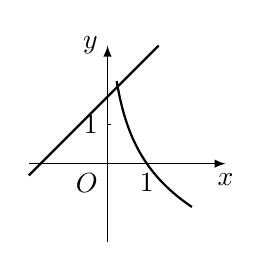
\begin{tikzpicture}[scale = 0.5,>=latex]
    \draw [->] (-2,0) -- (3,0) node [below] {$x$};
    \draw [->] (0,-2) -- (0,3) node [left] {$y$};
    \draw (0,0) node [below left] {$O$};
    \draw (0.1,1) -- (0,1) node [left] {$1$};
    \draw (1,0) node [below] {$1$};
    \draw [thick] (-2,-0.3) -- (1.3,3);
    \draw [thick,domain =-1.1:2.1,samples = 200] plot ({0.5^\x},\x);
\end{tikzpicture}
}{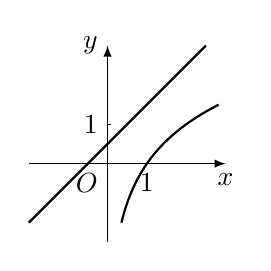
\begin{tikzpicture}[scale = 0.5,>=latex]
    \draw [->] (-2,0) -- (3,0) node [below] {$x$};
    \draw [->] (0,-2) -- (0,3) node [left] {$y$};
    \draw (0,0) node [below left] {$O$};
    \draw (0.1,1) -- (0,1) node [left] {$1$};
    \draw (1,0) node [below] {$1$};
    \draw [thick] (-2,-1.5) -- (2.5,3);
    \draw [thick,domain =1.5:-1.5,samples = 200] plot ({0.5^\x},-\x);
\end{tikzpicture}
}{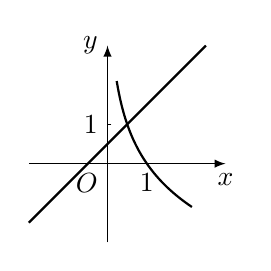
\begin{tikzpicture}[scale = 0.5,>=latex]
    \draw [->] (-2,0) -- (3,0) node [below] {$x$};
    \draw [->] (0,-2) -- (0,3) node [left] {$y$};
    \draw (0,0) node [below left] {$O$};
    \draw (0.1,1) -- (0,1) node [left] {$1$};
    \draw (1,0) node [below] {$1$};
    \draw [thick] (-2,-1.5) -- (2.5,3);
    \draw [thick,domain =-1.1:2.1,samples = 200] plot ({0.5^\x},\x);
\end{tikzpicture}
}{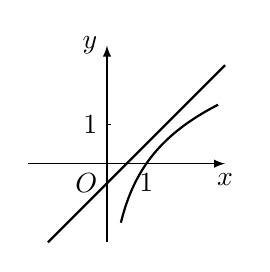
\begin{tikzpicture}[scale = 0.5,>=latex]
    \draw [->] (-2,0) -- (3,0) node [below] {$x$};
    \draw [->] (0,-2) -- (0,3) node [left] {$y$};
    \draw (0,0) node [below left] {$O$};
    \draw (0.1,1) -- (0,1) node [left] {$1$};
    \draw (1,0) node [below] {$1$};
    \draw [thick] (-1.5,-2) -- (3,2.5);
    \draw [thick,domain =1.5:-1.5,samples = 200] plot ({0.5^\x},-\x);
\end{tikzpicture}
}
\item {\tiny (000070)}选择题:\\
(1) 若$m>n>1$, 而$0<x<1$, 则下列不等式正确的是\bracket{20}.
\fourch{$m^x<n^x$}{$x^m<x^n$}{$\log_x m>\log_x n$}{$\log_m x<\log_n x$}
(2) 在同一平面直角坐标系中, 二次函数$y=ax^2+bx$与指数函数$y=(\dfrac ba)^x$的图像关系可能为\bracket{20}.
\fourch{
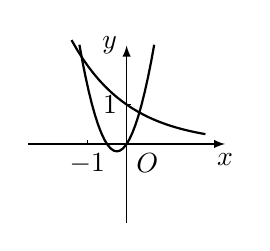
\begin{tikzpicture}[scale = 0.5, >=latex]
    \draw [->] (-2.5,0) -- (2.5,0) node [below] {$x$};
    \draw [->] (0,-2.) -- (0,2.5) node [left] {$y$};
    \draw (0,0) node [below right] {$O$};
    \draw (-1,0.1) -- (-1,0) node [below] {$-1$};
    \draw (0.1,1) -- (0,1) node [left] {$1$};
    \draw [domain = -1.2:0.7,thick] plot (\x,{3*\x * (\x+0.5)});
    \draw [domain = -1.4:2,thick] plot (\x,{(0.5)^\x}); 
\end{tikzpicture}
}{
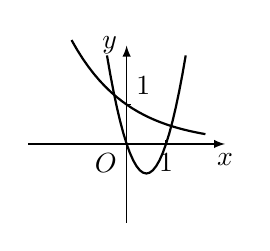
\begin{tikzpicture}[scale = 0.5, >=latex]
    \draw [->] (-2.5,0) -- (2.5,0) node [below] {$x$};
    \draw [->] (0,-2.) -- (0,2.5) node [left] {$y$};
    \draw (0,0) node [below left] {$O$};
    \draw (1,0.1) -- (1,0) node [below] {$1$};
    \draw (0.1,1) -- (0,1) node [above right] {$1$};
    \draw [domain = -0.5:1.5,thick] plot (\x,{3*\x*(\x-1)});
    \draw [domain = -1.4:2,thick] plot (\x,{(0.5)^\x}); 
\end{tikzpicture}
}{
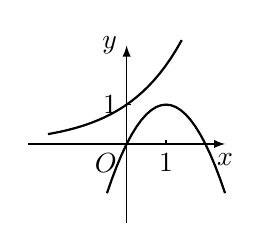
\begin{tikzpicture}[scale = 0.5, >=latex]
    \draw [->] (-2.5,0) -- (2.5,0) node [below] {$x$};
    \draw [->] (0,-2.) -- (0,2.5) node [left] {$y$};
    \draw (0,0) node [below left] {$O$};
    \draw (1,0.1) -- (1,0) node [below] {$1$};
    \draw (0.1,1) -- (0,1) node [left] {$1$};
    \draw [domain = -0.5:2.5,thick] plot ({\x},{-\x*(\x-2)});
    \draw [domain = -1.4:2,thick] plot ({-\x},{(0.5)^\x}); 
\end{tikzpicture}
}{
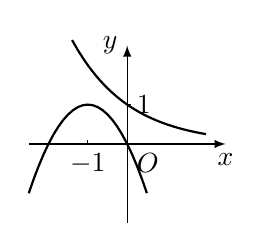
\begin{tikzpicture}[scale = 0.5, >=latex]
    \draw [->] (-2.5,0) -- (2.5,0) node [below] {$x$};
    \draw [->] (0,-2.) -- (0,2.5) node [left] {$y$};
    \draw (0,0) node [below right] {$O$};
    \draw (-1,0.1) -- (-1,0) node [below] {$-1$};
    \draw (0.1,1) -- (0,1) node [right] {$1$};
    \draw [domain = -2.5:0.5,thick] plot ({\x},{-\x*(\x+2)});
    \draw [domain = -1.4:2,thick] plot ({\x},{(0.5)^\x}); 
\end{tikzpicture}   
}
\item {\tiny (000355)}有以下命题:\\
\textcircled{1} 若函数$f(x)$既是奇函数又是偶函数, 则$f(x)$的值域为$\{0\}$; \\
\textcircled{2} 若函数$f(x)$是偶函数, 则$f(|x|)=f(x)$;\\
\textcircled{3} 若函数$f(x)$在其定义域内不是单调函数, 则$f(x)$不存在反函数;\\
\textcircled{4} 若函数$f(x)$存在反函数${{f}^{-1}}(x)$, 且${{f}^{-1}}(x)$与$f(x)$不完全相同, 则$f(x)$与${{f}^{-1}}(x)$图像的公共点必在直线$y=x$上; \\
其中真命题的序号是\blank{50}(写出所有真命题的序号).
\item {\tiny (000675)}已知定义在$\mathbf{R}$上的函数$f(x)$满足: \textcircled{1} $f(x)+f(2-x)=0$; \textcircled{2} $f(x)-f(-2-x)=0$; \textcircled{3} 在$[-1,1]$上的表达式为$f(x)=\begin{cases} \sqrt{1-x^2}, & x\in [-1,0], \\ 1-x, & x\in (0,1] \end{cases}$, 则函数$f(x)$与函数$g(x)=\begin{cases} 2^x, & x\le 0, \\ \log_{\frac12} x,& x>0 \end{cases}$的图像在区间$[-3,3]$上的交点的个数为\blank{50}.
\item {\tiny (000734)}给出下列函数: \textcircled{1} $y=x+\dfrac1x$; \textcircled{2} $y={x^2}+x$; \textcircled{3} $y={2^{|x|}}$; \textcircled{4} $y={x^{\dfrac23}}$; \textcircled{5} $y=\tan x$; \textcircled{6} $y=\sin(\arccos x)$; \textcircled{7} $y=\lg(x+\sqrt{{x^2}+4})-\lg 2$. 从这$7$个函数中任取两个函数, 则其中一个是奇函数另一个是偶函数的概率是\blank{50}.
\item {\tiny (001157)}设$A=\mathbf{Z}$, $B=\{n|n=2k+1,\ k\in \mathbf{Z}\}$, $C=\mathbf{R}$. $f:\ A\rightarrow B;\ x\mapsto 2x-1$, $g:\ B\rightarrow C;\ x\mapsto \dfrac{1}{2x+1}$. 经过两次映射,\\ 
(1) 求$A$中元素$1$在$C$中的对应元素;\\ 
(2) $C$中元素$1$在$A$中有没有对应元素?\\ 
(3) 如果把这两次映射``合成''成为一个$A$到$C$的映射$h$, 试写出$h$的对应法则.
\item {\tiny (001158)}(1) 试证明: 映射
\begin{align*}
f:\ [0,2]&\rightarrow \mathbf{R}\\
x&\mapsto x^2
\end{align*}
的像集为$[0,4]$;\\ 
(2) 试证明: 映射
\begin{align*}
f:\ [-1,2]&\rightarrow \mathbf{R}\\
x& \mapsto x^2
\end{align*}
的像集为$[0,4]$.
\item {\tiny (001161)}下列两个函数是同一个函数的有\blank{50}.\\ 
(1) $y=\dfrac{x^2-1}{x-1}$与$y=x+1$;\\ 
(2) $y=\dfrac{x^3}{x}$与$y=x^2$;\\ 
(3) $y=\sqrt{x^2}-1$与$y=\sqrt[3]{x^3}-1$;\\ 
(4) $f(x)=x^2-2x-1$与$g(t)=t^2-2t-1$;\\ 
(5) $f(x)=2^x, \ x \in \{0,1,2,3\}$与$g(x)=\dfrac16x^3+\dfrac56x+1, \ x \in \{0,1,2,3\}$.
\item {\tiny (001164)}写出下列函数的定义域(写在对应关系的右边):\\ 
(1) $f(x)=\dfrac{6}{x^2-3x+2}$;\\ 
(2) $f(x)=\dfrac{3x-1}{2x^3+4x^2+x-7}$;\\ 
(3) $f(x)=\dfrac{\sqrt[3]{4x+8}}{\sqrt{3x-2}}$;\\ 
(4) $f(x)=\sqrt{2x-1}+\sqrt{1-2x}+4$;\\ 
(5) $f(x)=\sqrt{x^2-4}$;\\ 
(6) $f(x)=\dfrac{\sqrt{2x+1}}{x-3}$.
\item {\tiny (001165)}(1) 函数$f(x)=x^2, \ x \in [0,1]$的值域为\blank{50};\\ 
(2) 函数$f(x)=-x, \ x \in [-1,0)$的值域为\blank{50};\\ 
(3) 函数$f(x)=\left\{\begin{array}{cc}x^2,&0\le x\le 1,\\-x,&-1\le x<0.\end{array}\right.$的值域为\blank{50}.
\item {\tiny (001172)}某物流公司在上海, 杭州各有库存的某种机器$12$台和$6$台, 现销售给A市$10$台, B市$8$台. 已知调运一台机器的运费(单位: 万元)如下表.
\begin{center}\begin{tabular}{c|cc}
&上海& 杭州\\
\hline
A市 & $4$ & $3$\\
B市 & $8$ & $5$
\end{tabular}\end{center}
设从上海往A市调运$x$台, 写出总运费$W$(单位: 万元)关于$x$的函数, 并求出怎样调运最节省运费.
\item {\tiny (001173)}在以下坐标系中分别作出下列函数的图像(用铅笔, 要求清晰, 交代关键信息):\\ 
\begin{tabular}{ll}
(1) $y=\sqrt{|x|}$;& (2) $y=|x-1|-|x+1|$;\\
\begin{tikzpicture}[>=latex]
    \foreach \i in {-4,-3,...,4} {\draw [dashed, gray!90] (-4,\i) -- (4,\i) (\i,-4) -- (\i,4);};
    \draw [->] (-4,0) -- (4,0) node [below] {$x$};
    \draw [->] (0,-4) -- (0,4) node [left] {$y$};
    \draw (0,0) node [below left] {$O$};
    \draw (0,1) node [left] {$1$};
    \draw (1,0) node [below] {$1$};
\end{tikzpicture} & 
\begin{tikzpicture}[>=latex]
    \foreach \i in {-4,-3,...,4} {\draw [dashed, gray!90] (-4,\i) -- (4,\i) (\i,-4) -- (\i,4);};
    \draw [->] (-4,0) -- (4,0) node [below] {$x$};
    \draw [->] (0,-4) -- (0,4) node [left] {$y$};
    \draw (0,0) node [below left] {$O$};
    \draw (0,1) node [left] {$1$};
    \draw (1,0) node [below] {$1$};
\end{tikzpicture}
\end{tabular}
\begin{tabular}{ll}
(3) $y=x-[x]$;& (4) $y=x+\dfrac{1}{x}$;\\
\begin{tikzpicture}[>=latex]
    \foreach \i in {-4,-3,...,4} {\draw [dashed, gray!90] (-4,\i) -- (4,\i) (\i,-4) -- (\i,4);};
    \draw [->] (-4,0) -- (4,0) node [below] {$x$};
    \draw [->] (0,-4) -- (0,4) node [left] {$y$};
    \draw (0,0) node [below left] {$O$};
    \draw (0,1) node [left] {$1$};
    \draw (1,0) node [below] {$1$};
\end{tikzpicture} & 
\begin{tikzpicture}[>=latex]
    \foreach \i in {-4,-3,...,4} {\draw [dashed, gray!90] (-4,\i) -- (4,\i) (\i,-4) -- (\i,4);};
    \draw [->] (-4,0) -- (4,0) node [below] {$x$};
    \draw [->] (0,-4) -- (0,4) node [left] {$y$};
    \draw (0,0) node [below left] {$O$};
    \draw (0,1) node [left] {$1$};
    \draw (1,0) node [below] {$1$};
\end{tikzpicture}
\end{tabular}
\begin{tabular}{ll}
(5) $y=x-\dfrac{1}{x}$;& (6) $y=\dfrac{6x}{1+x^2}$.\\
\begin{tikzpicture}[>=latex]
    \foreach \i in {-4,-3,...,4} {\draw [dashed, gray!90] (-4,\i) -- (4,\i) (\i,-4) -- (\i,4);};
    \draw [->] (-4,0) -- (4,0) node [below] {$x$};
    \draw [->] (0,-4) -- (0,4) node [left] {$y$};
    \draw (0,0) node [below left] {$O$};
    \draw (0,1) node [left] {$1$};
    \draw (1,0) node [below] {$1$};
\end{tikzpicture} & 
\begin{tikzpicture}[>=latex]
    \foreach \i in {-4,-3,...,4} {\draw [dashed, gray!90] (-4,\i) -- (4,\i) (\i,-4) -- (\i,4);};
    \draw [->] (-4,0) -- (4,0) node [below] {$x$};
    \draw [->] (0,-4) -- (0,4) node [left] {$y$};
    \draw (0,0) node [below left] {$O$};
    \draw (0,1) node [left] {$1$};
    \draw (1,0) node [below] {$1$};
\end{tikzpicture}
\end{tabular}
\item {\tiny (001174)}某种茶杯每个$0.5$元, 买$x$个茶杯的钱数为$y$元. 画出$y$关于$x$的函数的图像.\\ 
\begin{tikzpicture}[>=latex]
    \foreach \i in {0,1,...,7} {\draw [dashed, gray!90] (0,\i) -- (16,\i);};
    \foreach \i in {0,1,...,16} {\draw [dashed, gray!90] (\i,0) -- (\i,7);};
    \draw [->] (-0.5,0) -- (16,0) node [below] {$x$};
    \draw [->] (0,-0.5) -- (0,7) node [left] {$y$};
    \draw (0,0) node [below left] {$O$};
    \draw (0,1) node [left] {$1$};
    \draw (1,0) node [below] {$1$};
\end{tikzpicture}
\item {\tiny (001178)}试求出函数$y=\sqrt{x}$的图像分别进行如下变换后所得的各个图像对应的函数.\\ 
(1) 图像上的每一点的横坐标变为原来的$2$倍;\\ 
(2) 图像上的每一点的纵坐标变为原来的$\dfrac{1}{2}$;\\ 
(3) 图像上的每一点的横坐标变为原来的$2$倍, 然后向上平移$3$个单位, 所得图像上每一点的纵坐标变为原来的$3$倍, 再向左平移$2$个单位;\\ 
(4) 向左平移$3$个单位, 然后将所得图像上的每一点的横坐标变为原来的$\dfrac{1}{2}$, 最后向下平移$2$个单位
\item {\tiny (001187)}求以下各函数的复合.\\ 
(1) $f(x)=2x$, $g(x)=\dfrac{x}{2}$, 求$f\circ g$, $g\circ f$;\\ 
(2) $f(x)=\sqrt{x}$, $g(x)=2x+1$, 求$f\circ g$, $g\circ f$;\\ 
(3) $f(x)=x^3+1$, $g(x)=\sqrt[3]{x-1}$, 求$f\circ f$, $f\circ g$, $g\circ f$;\\ 
(4) $f(x)=x+1,\ x \in [1,+\infty)$, $g(x)=x-1, \  x \in (-\infty,3]$, 求$f\circ g$, $g\circ f$.
\item {\tiny (001190)}下列各映射中, 是单射的有\blank{60}, 是满射的有\blank{60}, 存在逆映射的有\blank{60}.\\ 
\textcircled{1} $f: \{1,2,3\}\rightarrow \{1,4,9\}; \ x\mapsto x^2$;\\ 
\textcircled{2} $f: \mathbf{R}^+\rightarrow \mathbf{R}^+; \ x \mapsto x^2$;\\ 
\textcircled{3} $f: \mathbf{R}\rightarrow [0,+\infty); \ x \mapsto x^2$;\\ 
\textcircled{4} $f: \mathbf{R}^+\rightarrow \mathbf{R}^+; \ x \mapsto \dfrac{1}{x}$;\\ 
\textcircled{5} $f: \mathbf{R}^+\cup \mathbf{R}^-\rightarrow \mathbf{R}^+\cup \mathbf{R}^-; \ x \mapsto \dfrac{1}{x}$;\\ 
\textcircled{6} $f: \mathbf{R}^+\rightarrow \mathbf{R}; \ x \mapsto x+\dfrac{1}{x}$;\\ 
\textcircled{7} $f: \mathbf{R}^+\rightarrow \mathbf{R}; \ x \mapsto x-\dfrac{1}{x}$;\\ 
\textcircled{8} $f: \mathbf{R}\rightarrow \mathbf{Z}; \ x \mapsto [x]$;\\ 
\textcircled{9} $f: \{(x,y)|x,y\in \mathbf{R}\}\rightarrow \{(x,y)|x,y\in \mathbf{R}\};\ (x,y)\mapsto (x+y,x-y)$;\\ 
\textcircled{10} $f: \{(x,y)|x,y\in \mathbf{R}\}\rightarrow \{(x,y)|x,y\in \mathbf{R}\};\ (x,y)\mapsto (x+y,2x+2y)$.
\item {\tiny (001192)}写出下列函数的反函数(注意定义域).\\ 
(1) $y=-\dfrac{1}{x}+3$;\\ 
(2) $y=\sqrt{2x-1}$;\\ 
(3) $y=\dfrac{2x+1}{x+2}$;\\ 
(4) $y=x^2+2, \ x\in [2,+\infty)$;\\ 
(5) $y=2^x, \ x\in \{1,2,3,4\}$ (本小题不能使用对数);\\ 
(6) $y=\sqrt{9-x^2}, \ x\in [-3,0]$;\\ 
(7) $y=x^2-4x, x \in [3,7]$.
\item {\tiny (001198)}在同一坐标系中通过平移和放缩作出以下函数的图像, 并写出变换的方法.
$y=|x|$; $y=|x-1|$; $y=\dfrac{|x-1|}2$; $y=\dfrac{|x-1|}2-3$; $y=\dfrac{|2x-1|}2-3$.
\begin{center}
\begin{tikzpicture}[>=latex]
    \foreach \i in {-4,-3,...,4} {\draw [dashed, gray!90] (-4,\i) -- (4,\i) (\i,-4) -- (\i,4);};
    \draw [->] (-4,0) -- (4,0) node [below] {$x$};
    \draw [->] (0,-4) -- (0,4) node [left] {$y$};
    \draw (0,0) node [below left] {$O$};
    \draw (0,1) node [left] {$1$};
    \draw (1,0) node [below] {$1$};
\end{tikzpicture}
\end{center}
\item {\tiny (001213)}已知函数$y=f(x)$与$y=g(x)$的定义域均为$\mathbf{R}$.\\ 
\blank{25}(1) 如果$y=f(x)$是奇函数, 那么$y=|f(x)|$是偶函数;\\ 
\blank{25}(2) 如果$y=f(x)$是奇函数, 那么$y=\sqrt[3]{f(x)}$是奇函数;\\ 
\blank{25}(3) 如果$y=f(x)$是奇函数, 那么$y=f(|x|)$是奇函数;\\ 
\blank{25}(4) 如果$y=f(x)$是奇函数, 那么$y=f(|x|)$是偶函数;\\ 
\blank{25}(5) 如果$y=f(x)$是奇函数, $y=g(x)$是偶函数, 那么$y=f(x)g(x)$是奇函数;\\ 
\blank{25}(6) 如果$y=f(x)$是奇函数, $y=g(x)$不是偶函数, 那么$y=f(x)+2g(x)$既非奇函数又非偶函数;\\ 
\blank{25}(7) 如果$y=f(x)$不是奇函数, $y=g(x)$也不是奇函数, 那么$y=f(x)-g(x)$也不是奇函数;\\ 
\blank{25}(8) 如果$y=f(x)$是奇函数, $y=g(x)$不是偶函数, 那么$y=f(x)+g(x)$不是偶函数;\\ 
\blank{25}(9) 如果$y=f(x)-g(x)$是奇函数, $y=g(x)$是奇函数, 那么$y=f(x)$也是奇函数;\\ 
\blank{25}(10) 如果$y=(f(x))^2$是偶函数, 那么$y=f(x)$是偶函数或者是奇函数;\\ 
\blank{25}(11) 如果$y=(f(x))^2$是奇函数, 那么$y=f(x)$恒等于零, 因此是奇函数也是偶函数;\\ 
\blank{25}(12) 如果$y=(f(x))^3$是奇函数, 那么$y=f(x)$是奇函数.
\item {\tiny (001214)}已知函数$y=f(x),\ x \in D_f$与$y=g(x),\ x \in D_g$的定义域交集非空.\\ 
\blank{25}(1) 如果$y=f(x)$是奇函数, $y=g(x)$是奇函数, 那么$y=f(x)+x^2g(x)$是奇函数;\\ 
\blank{25}(2) 如果$y=f(x)$是奇函数, $y=g(x)$是偶函数, 而且它们都不恒等于零, 那么$y=f(x)+g(x)$既不是奇函数又不是偶函数;\\ 
\blank{25}(3) 如果$y=f(x)$是奇函数, $y=g(x)$是偶函数, 而且它们在$D_f\cap D_g$上都不恒等于零, 那么$y=f(x)+g(x)$既不是奇函数又不是偶函数;\\ 
\blank{25}(4) 如果$y=f(x)$不是奇函数, $y=g(x)$也不是奇函数, 那么$y=f(x)-g(x)$也不是奇函数;\\ 
\blank{25}(5) 如果$y=|f(x)|$是奇函数, 那么$f(x)$恒等于零;\\ 
\blank{25}(6) 如果$y=f(x)$不是奇函数, 那么$y=|f(x)|$不是偶函数;\\ 
\blank{25}(7) 如果$y=f(x)$是偶函数, 且$y=f(x)+g(x)$也是偶函数, 那么$y=g(x)$也是偶函数.
\item {\tiny (001215)}已知$y=f(x), \ x \in D$是偶函数.\\ 
\blank{25}(1) $y=(f(x))^3+f(x)$是偶函数;\\ 
\blank{25}(2) $y=f(2x)$是偶函数;\\ 
\blank{25}(3) $y=f(x-1)$的图像关于直线$x=-1$对称;\\ 
\blank{25}(4) $y=f(x-1)$的图像关于直线$x=1$对称;\\ 
\blank{25}(5) $y=f(3x+1)$的图像关于直线$x=-\dfrac{1}{3}$对称;\\ 
\blank{25}(6) $y=f(3x+1)$的图像关于直线$x=-1$对称;\\ 
\blank{25}(7) $y=f(x^3+1)$是偶函数;\\ 
\blank{25}(8) $y=f(x^3+x)$是偶函数.
\item {\tiny (001216)}已知$y=f(x)$是奇函数.\\ 
\blank{25}(1) $y=f(3x)$是奇函数;\\ 
\blank{25}(2) $y=f(x-1)+2$的图像关于点$(1,2)$对称;\\ 
\blank{25}(3) $y=3f(2x-1)+6$的图像关于点$(1,6)$对称;\\ 
\blank{25}(4) $y=3f(2x-1)+6$的图像关于点$(\dfrac{1}{2},6)$对称;\\ 
\blank{25}(5) $y=3f(2x-1)+6$的图像关于点$(\dfrac{1}{2},2)$对称;\\ 
\blank{25}(6) $y=f(x^2)$是偶函数;\\ 
\blank{25}(7) $y=f^{-1}(x)$一定存在;\\ 
\blank{25}(8) $y=f^{-1}(x)$如果存在, 则必定是奇函数.
\item {\tiny (001217)}已知$y=f(x)$在$\mathbf{R}$上是增函数.\\ 
\blank{25}(1) 如果$y=g(x)$在区间$I$上递增, 则$y=f(x)+g(x)$在区间$I$上递增;\\ 
\blank{25}(2) 如果$y=g(x)$在区间$I$上递增, 则$y=f(x)g(x)$在区间$I$上递增;\\ 
\blank{25}(3) 如果$y=g(x)$在区间$I$上递增, 则$y=f(g(x))$在区间$I$上递增;\\ 
\blank{25}(4) 如果$y=g(x)$在区间$I$上递增, 则$y=g(f(x))$在$\mathbf{R}$上递增;\\ 
\blank{25}(5) 如果$y=g(x)$满足$y=f(x)-g(x)$在$\mathbf{R}$上递增, 那么$y=g(x)$在$\mathbf{R}$上递减;\\ 
\blank{25}(6) 如果$y=g(x)$满足$y=f(x)-g(x)$在$\mathbf{R}$上递减, 那么$y=g(x)$在$\mathbf{R}$上递减;\\ 
\blank{25}(7) 如果定义在$\mathbf{R}$上的函数$y=g(x)$满足$y=g(f(x))$在$\mathbf{R}$上递增, 则$y=g(x)$在$\mathbf{R}$上递增;\\ 
\blank{25}(8) 如果定义在$\mathbf{R}$上的函数$y=g(x)$满足$y=g(f(x))$在$\mathbf{R}$上递减, 则$y=g(x)$在$\mathbf{R}$上递减.
\item {\tiny (001222)}是非题, 在每个命题之前的横线上写上``T''或``F''即可, 不用写任何原因.\\ 
已知$y=f(x)$是定义在区间$[-1,1]$上的函数.\\ 
\blank{25}(1) 如果$f(x)$是奇函数, 则$f(x)$要么是增函数, 要么是减函数;\\ 
\blank{25}(2) 如果$f(x)$是偶函数, 则$f(x)$既不是增函数, 又不是减函数;\\ 
\blank{25}(3) 如果$f(x)$是奇函数, 且在$[0,1]$上递增, 那么$f(x)$在$[-1,0]$上也递增;\\ 
\blank{25}(4) 如果$f(x)$是奇函数, 且在$[0,1]$上递增, 那么$f(x)$在$[-1,1]$上也递增;\\ 
\blank{25}(5) 如果$f(x)$在$[-1,0),[-\dfrac{1}{2},\dfrac{1}{2}],(0,1]$上都是递增的, 那么$f(x)$ 在$[-1,1]$上也递增.
\item {\tiny (001223)}是非题, 在每个命题之前的横线上写上``T''或``F''即可, 不用写任何原因.\\ 
已知$y=f(x)$是定义在$[-1,1]$上的偶函数, 在$[0,1]$上递增.\\ 
\blank{25}(1) $f(\dfrac{1}{2})>f(-\dfrac{1}{3})$;\\ 
\blank{25}(2) $f(a)>f(b)$当且仅当$a>b$;\\ 
\blank{25}(3) $f(a)>f(b)$当且仅当$|a|>|b|$;\\ 
\blank{25}(4) $f(a)>f(b)$当且仅当$1\ge |a|>|b|$.
\item {\tiny (001226)}(1) 函数$y=1-x^2, \ x\in [-1,1]$的最大值为\blank{50}, 最小值为\blank{50}, 最大值点为\blank{50}, 最小值点为\blank{50};\\ 
(2) 函数$y=2x^2-8x, \ x\in [-1,4]$的最大值为\blank{50}, 最小值为\blank{50}, 最大值点为\blank{50}, 最小值点为\blank{50};\\ 
(3) 函数$y=6x-x^2, \ x\in [-3,0]$的最大值为\blank{50}, 最小值为\blank{50}, 最大值点为\blank{50}, 最小值点为\blank{50};\\ 
(4) 函数$y=2x^2-4x+5, \ x\in [2,4]$的最大值为\blank{50}, 最小值为\blank{50}, 最大值点为\blank{50}, 最小值点为\blank{50}.
\item {\tiny (001227)}(1) 函数$y=x+\dfrac{4}{x}, \ x\in [1,5]$的最大值为\blank{50}, 最小值为\blank{50}, 最大值点为\blank{50}, 最小值点为\blank{50};\\ 
(2) 函数$y=x-\dfrac{4}{x}, \ x\in [1,5]$的最大值为\blank{50}, 最小值为\blank{50}, 最大值点为\blank{50}, 最小值点为\blank{50};\\ 
(3) 函数$y=\dfrac{x-5}{3x+2}, \ x\in [0,3]$的最大值为\blank{50}, 最小值为\blank{50}, 最大值点为\blank{50}, 最小值点为\blank{50};\\ 
(4) 函数$y=x^2+\dfrac{16}{x}, \ x\in [1,4]$的最大值为\blank{50}, 最小值为\blank{50}, 最大值点为\blank{50}, 最小值点为\blank{50}.
\item {\tiny (001266)}写出下列函数的值域.\\ 
(1) $y=3x+1, \ x \in [-2,5]$; \blank{80}\\ 
(2) $y=|2x+1|, \ x \in [-1,3]$; \blank{80}\\ 
(3) $y=\dfrac{x-1}{2x+3}$; \blank{80}\\ 
(4) $y=\dfrac{|x|+1}{|x|-1}$; \blank{80}\\ 
(5) $y=\dfrac{|x+3|}{x-4}, \ x \in [-4,0]$; \blank{80}\\ 
(6) $y=\dfrac{2x+1}{|x+1|-|x|}$; \blank{80}
\item {\tiny (001271)}写出下列函数的值域:\\ 
(1) $y=x^2+2x+2$; \blank{80}\\ 
(2) $y=-x^2+3x+4$; \blank{80}\\ 
(3) $y=4x^2+x+1, \ x \in [-3,0]$; \blank{80}\\ 
(4) 已知$a>0$, $y=ax^2+ax+2a, \ x \in [-1,1)$; \blank{80}\\ 
(5) $y=\dfrac{1}{x^2+2x+2}$; \blank{80}\\ 
(6) $y=4-\sqrt{4x-4x^2}$; \blank{80}\\ 
(7) $y=\dfrac{x^2-x-2}{x^2+3x+2}$; \blank{80}\\ 
(8) $y=|x^2-2x-3|, \ x \in (\dfrac{1}{2},2]$; \blank{80}
\item {\tiny (001279)}已知$m$是实数, 试就关于$x$的方程$x^2-mx+2m-2=0$的两个实数根(重根算两个根)的不同分布情况, 确定$m$的范围(只要写答案).
\begin{multicols}{2}
(1) 两根分别在$(-\infty,0)$和$(0,+\infty)$中;\\ 
(3) 两根分别在$(-\infty,\dfrac{3}{2})$和$(\dfrac{3}{2},+\infty)$中;\\ 
(5) 两根在$(0,\dfrac{3}{2})$中;\\ 
(7) 在$(0,\dfrac{3}{2})$内有且仅有一个根;\\ 
(9) 在$[0,\dfrac{3}{2}]$内有两个根;\\ 
(11) 在$[0,\dfrac{3}{2}]$内有根;\\ 
(2) 两根均在$(0,+\infty)$中;\\ 
(4) 两根均在$(-\infty,\dfrac{3}{2})$中;\\ 
(6) 在$(0,\dfrac{3}{2})$内有且仅有一个根, 且$0,\dfrac{3}{2}$均不是根;\\ 
(8) 在$(0,\dfrac{3}{2})$内有根;\\ 
(10) 在$[0,\dfrac{3}{2}]$内有且仅有一个根;\\ 
(12) 两根分别在$(-\infty,0)$和$(\dfrac{3}{2},+\infty)$中.\\ 
\end{multicols}
\item {\tiny (001281)}已知$a$是实数, 就关于$x$的方程$x^2+(a-5)x+(a-2)=0$的两个根(重根算两个根)的不同分布情况, 利用函数$y=\dfrac{-x^2+5x+2}{x+1}$的图像与性质确定$a$的范围.\\ 
\begin{multicols}{2}
(1) 两个根分别在$(-\infty,2)$和$(2,+\infty)$中;\\ 
(3) 有根在$[0,2)$内;\\ 
(2) 两个根都在$(-\infty,-2)$中;\\ 
(4) 有两个不同的根, 有且仅有一根在$[0,+\infty)$中.\\ 
\end{multicols}
\item {\tiny (001300)}用不含对数的式子表示:\\ 
(1) 若$\log_7 2=a$, 则$\log_7 14=$\blank{80}, $\log_7 \sqrt{3.5}=$\blank{80}.\\ 
(2) 若$\log_3 2=a$, 则$\log_3 4=$\blank{80}, $\log_3 \dfrac{2}{3}=$\blank{80}.\\ 
(3) 若$\lg 2=a$, 则$\lg 25=$\blank{80}.
\item {\tiny (001305)}计算下列各式(要有必要的过程):\\
(1) $\dfrac{1}{2}\log_{20}45-\log_{20}30$;\\ 
(2) $\dfrac{\lg3+\dfrac{2}{5}\lg9+\dfrac{3}{5}\lg\sqrt{27}-\lg\sqrt{3}}{\lg81-\lg27}$;\\ 
(3) $\lg^22+\lg^25+2\lg2\lg5$; \\ 
(4) $\lg^32+\lg^35+3\lg2\lg5$; \\
(5) $\lg4+2\sqrt{\lg^26-\lg6^2+1}+\lg9$.
\item {\tiny (001312)}计算下列各式(要有必要的过程):\\ 
(1) $\log_3 5\cdot\log_5 7\cdot\log_7 9$; \\ 
(2) $(\log_4 3+\log_8 3)(\log_3 2+\log_9 2)$;\\ 
(3) $2\log_{100} 5-\sqrt{1-2\lg2+\lg^2 2}$; \\ 
(4) $\dfrac{\log_5 \sqrt{2}\cdot\log_7 9}{\log_5\dfrac{1}{3}\cdot\log_7\sqrt[3]{4}}$;\\
(5) $2^{\log_4(\sqrt{3}-2)^2}+3^{\log_9(\sqrt{3}+2)^2}$;\\ 
(6) $\dfrac{\log_{36}4}{\log_{18}6}+\log_6^2 3$.
\item {\tiny (001320)}已知$f_1(x)=3^x-1$, $f_2(x)=3^{x-1}$, $f_3(x)=-3^x$, $f_4(x)=-3^{-x}$, $f_5(x)=(1/3)^x$, $f_6(x)=(1/3)^{-x}$. 则将函数$y=3^x$的图像右移$1$单位得\blank{80}的图像, 下移$1$单位得\blank{80}的图像. $y=3^x$的图像与\blank{80}的图像关于$x$轴对称, 与\blank{80}的图像关于$y$轴对称, 与$\blank{80}$的图像关于原点对称, 与\blank{80}的图像完全相同.
\item {\tiny (001337)}作出下列函数的大致图像(只要能够表明定义域和单调性, 凹凸性方面的信息):\\ 
\begin{multicols}{2}
(1) $y=x^{\frac{2}{3}}$; \\ 
(2) $y=x^{-\frac{3}{2}}$; \\ 
\end{multicols}
\begin{multicols}{2}
(3) $y=\dfrac{|x|+1}{|x+1|}$;  \\ 
(4) $y=\dfrac{1}{(x-2)^2}-1$.
\end{multicols}
\item {\tiny (001340)}在下列幂函数 (1) $y=x^{-\frac{3}{2}}$, (2) $y=x^{\frac{5}{4}}$, (3) $y=x^{-\frac{4}{3}}$, (4) $y=x^4$, (5) $y=x^{\frac{3}{7}}$, (6) $y=x^{-6}$中, 定义域关于原点对称的有\blank{80}, 值域为$\mathbf{R}$的有\blank{80}, 奇函数有$\blank{80}$, 在定义域上单调递增的有\blank{80}, 图像有一部分在第二象限的有\blank{80}.
\item {\tiny (002823)}下列各组中, 两个函数是同一个函数的组的序号是\blank{50}.\\
(1) $y=\lg x$与$y=\dfrac 12\lg {x^2}$; (2) $f(x)=2^x$, $D=\{0,1,2,3\}$与$g(x)=\dfrac 16{x^3}+\dfrac 56x+1$, $D=\{0,1,2,3\}$; \\
(3) $f(x)=x^2-2x-1$, $g(t)=t^2-2t-1$; (4) $y=\sqrt{x^2}-1$, $y=\sqrt[3]{x^3}-1$.
\item {\tiny (002827)}已知$y=f(x)$为偶函数, 且$y=f(x)$的图像在$x\in [0,1]$时的部分是半径为$1$的圆弧, 在$x\in [1,+\infty)$时的部分是过点$(2,1)$的射线, 如图.\\
\begin{center}
    \begin{tikzpicture}[>=latex]
        \draw [->] (-1,0) -- (4,0) node [below] {$x$};
        \draw [->] (0,-1) -- (0,3) node [left] {$y$};
        \draw (0,1) arc (90:0:1) -- (3,2);
        \draw (0,0) node [below left] {$O$};
        \draw (1,0) node [below] {$1$};
        \draw (0,1) node [left] {$1$};
        \draw [dashed] (2,0) -- (2,1) -- (0,1);
        \draw (2,0) node [below] {$2$};
    \end{tikzpicture}
\end{center}
(1) 写出函数$y=f(x)$在$x<0$时的单调性:\blank{50};\\
(2) 写出$f(f(-2))$的值:\blank{50};\\
(3) 写出方程$f(x)=\dfrac{\sqrt 3}2$的解集:\blank{50}.
\item {\tiny (002828)}某工厂生产一种仪器的元件, 由于受生产能力和技术水平等因素的限制, 会产生较多次品, 根据经验知道, 次品数$p$(万件)与日产量$x$(万件)之间满足关系: $p=\begin{cases}  \dfrac{x^2}6,  &1\le x<4, \\ x+\dfrac 3x-\dfrac{25}{12}, & x\ge 4. \end{cases}$ 已知每生产$1$万件合格的元件可以盈利$20$万元, 但每产生$1$万件次品将亏损$10$万元. ($\text{实际利润}=\text{合格产品的盈利}-\text{生产次品的亏损}$), 试将该工厂每天生产这种元件所获得的实际利润$T$(万元)表示为日产量$x$(万件)的函数.
\item {\tiny (002830)}如图, 用长为$l$的铁丝弯成下部为矩形, 上部为半圆形的空心框架, 若矩形底边长为$2x$, 试用解析式将此框架围成的面积$y$表示$x$的函数.
\begin{center}
    
\begin{tikzpicture}
        \draw (0,0) -- (2,0) -- (2,2.3) arc (0:180:1) -- cycle;
    \end{tikzpicture}
\end{center}
\item {\tiny (002834)}(1)设函数$D(x)=\begin{cases} 1, & x\in \mathbf{Q}, \\  0, &x\notin\mathbf{Q}. \end{cases}$ 令$F(x)=D(\sqrt 2x)$, 则$F(1)=$\blank{50};\\
(2) 已知函数$f(x)=\begin{cases} 2-x, & x<-2, \\ x^2, & -2\le x<1, \\ x, & x\ge 1. \end{cases}$ 若$f(x)=2$, 则$x$=\blank{50}.
\item {\tiny (002841)}已知常数$a\in \mathbf{R}$, 函数$g(x)=\dfrac x{x+2}$, 函数$h(x)=\dfrac 1{x+a}$. 设函数$F(x)=g(x)\cdot h(x)$, $D_F$是其定义域; $f(x)=g(x)-h(x)$, $D_f$是其定义域.\\
(1) 设$a=2$, 求函数$F(x)$的值域;\\
(2) 对于给定的常数$a$, 是否存在实数$t$, 使得$f(t)=0$成立? 若存在, 求出这样的所有$t$的值; 若不存在, 说明理由;\\
(3) *是否存在常数$a$的值, 使得对于任意$x\in {D_f}\cap \mathbf{R}^+$, 有$f(x)\ge 0$恒成立? 若存在, 求出所有这样的a的值; 若不存在, 说明理由.
\item {\tiny (002842)}给定六个函数: \textcircled{1} $y=\dfrac 1x$; \textcircled{2} $y=x^2+1$; \textcircled{3} $y={x^{-\frac 13}}$; \textcircled{4} $y=2^x$; \textcircled{5} $y=\log_2x$; \textcircled{6} $y=\sqrt{x^2-1}+\sqrt{1-x^2}$.\\
在这六个函数中, 是奇函数但不是偶函数的是\blank{50}, 是偶函数但不是奇函数的是\blank{50}, 既不是奇函数也不是偶函数的是\blank{50}, 既是奇函数又是偶函数的是\blank{50}.
\item {\tiny (002848)}设奇函数$y=f(x)$的定义域为$[-5, 5]$.若当$x\in [0,5]$时, $y=f(x)$的图像如图, 则不等式$xf(x)<0$的解是\blank{50}.
\begin{center}
    \begin{tikzpicture}[>=stealth]
        \draw [->] (-1,0) -- (6,0) node [below] {$x$};
        \draw [->] (0,-2.5) -- (0,2.5) node [left] {$y$};
        \draw (2,0) node [below] {$2$};
        \draw (5,0) node [above] {$5$};
        \draw [domain = 0:2,samples = 100] plot (\x,-\x*\x+2*\x);
        \draw [domain = 2:5,samples = 100] plot (\x, \x*\x/2-4*\x+6);
        \draw [dashed] (5,0) -- (5,-1.5);
        \draw (0,0) node [below left] {$O$};
    \end{tikzpicture}
\end{center}
\item {\tiny (002872)}设函数$y=f(x)$为$\mathbf{R}$上的奇函数, 且对于任意$x\in \mathbf{R}$都有$f(x+2)=-f(x)$.\\
(1) 求证: 函数$y=f(x)$为周期函数;\\
(2) 对于任意$x\in \mathbf{R}$, 求证: $f(1+x)=f(1-x)$;\\
(3) 设$0\le x\le 1$时, $f(x)=\dfrac 12x$. 求函数$y=f(x)+\dfrac 12$在$-4\le x\le 4$时的所有零点;\\
(4) 设$-1\le x\le 1$时, $f(x)=\sin x$.\\
\textcircled{1} 写出$1\le x\le 5$时, $y=f(x)$的解析式;\\
\textcircled{2} 求$y=f(x)$在$\mathbf{R}$上的解析式.
\item {\tiny (002879)}已知定义域为$\mathbf{R}$的函数$y=f(x)$是偶函数, 并且其图像关于直线$x=1$对称.\\
(1) 若$f(0)=1$, $f(1)=2$, 求$f(15)+2f(20)$的值;\\
(2) 设$x\in [0,1]$时, $f(x)=x^3$.\\
\textcircled{1} $1<x\le 2$时, 求$y=f(x)$的解析式;\\
\textcircled{2} $-2\le x<0$时, 求$y=f(x)$的解析式;\\
\textcircled{3} 求函数$y=f(x)-\dfrac 18$在$[-2,2]$上的所有零点;\\
\textcircled{4} 求$y=f(x)$在$\mathbf{R}$上的解析式.
\item {\tiny (002883)}*设定义在$\mathbf{R}$上的函数$y=f(x)$的满足: 对于任意$x\in \mathbf{R}$, 恒有$f(-x+1)=-f(x+1)$且$f(-x-1)=-f(x-1)$. 则下面命题中, 正确的命题的序号是\blank{50}.\\
\textcircled{1} 函数$y=f(x)$是偶函数; \textcircled{2} $2$是$y=f(x)$的周期; \textcircled{3} 函数$y=f(x)$图像关于$(1,0)$对称; \textcircled{4} 函数$y=f(x)$图像关于$(3,0)$对称.
\item {\tiny (002897)}下列函数中, 在区间$(0 ,+\infty)$上递增的函数的序号为\blank{50}.\\
\textcircled{1} $y=|x+1|$;  \textcircled{2} $y=x-\dfrac 1x$;    \textcircled{3} $y={x^{\frac 12}}$;    \textcircled{4} $y=\sqrt{1-\dfrac 1x}$; \textcircled{5} $y=\lg x$.
\item {\tiny (002906)}已知定义$\mathbf{R}$上的函数$y=f(x)$满足下面两个条件:\\
(I) 对于任意$x_1,x_2\in \mathbf{R}$, 都有$f(x_1+x_2)=f(x_1)+f(x_2)$; (II)当$x>0$时, $f(x)>0$, 且$f(1)=1$.\\
(1) 求证: $y=f(x)$是奇函数;\\
(2) 求证: $y=f(x)$在$\mathbf{R}$上是增函数;\\
(3) *解不等式$f(x^2-1)<2$.
\item {\tiny (002908)}下列命题中, 正确的命题的序号是\blank{50}.\\
\textcircled{1} 当$\alpha =0$时, 函数$y={x^{\alpha }}$的图像是一条直线;\\
\textcircled{2} 幂函数的图像都经过(0, 0)和(1, 1)点;\\
\textcircled{3} 当$\alpha <0$且$y={x^{\alpha }}$是奇函数时, 它也是减函数;\\
\textcircled{4} 第四象限不可能有幂函数的图像.
\item {\tiny (002909)}图中曲线是幂函数$y=x^n$在第一象限的图像, 已知$n$取$\pm 2$, $\pm\dfrac 12$四个值, 则相应于曲线$c_1,c_2,c_3,c_4$的$n$依次为\bracket{20}.
\begin{center}
    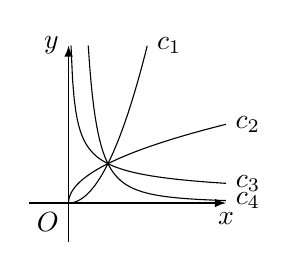
\begin{tikzpicture}[>=latex,scale = 0.5]
        \draw [->] (-1,0) -- (4,0) node [below] {$x$};
        \draw [->] (0,-1) -- (0,4) node [left] {$y$};
        \draw (0,0) node [below left] {$O$};
        \draw [domain = 0:2, samples = 100] plot (\x,\x*\x) node [right] {$c_1$};
        \draw [domain = 0:2, samples = 100] plot (\x*\x,\x) node [right] {$c_2$};
        \draw [domain = 0.0625:4, samples = 100] plot (\x, {1/sqrt(\x)}) node [right] {$c_3$};
        \draw [domain = 0.5:4, samples = 100] plot (\x, {1/\x/\x}) node [right] {$c_4$};
    \end{tikzpicture}
    \end{center}
\fourch{$-2,-\dfrac 12,\dfrac 12,2$}{$2,\dfrac 12,-\dfrac 12,-2$
}{$-\dfrac 12,-2,2,\dfrac 12$}{$2,\dfrac 12,-2,-\dfrac 12$}
\item {\tiny (002910)}下列函数的图像为(A)、(B)、(C)、(D)之一, 试将正确的字母标号填在相应函数后面的横线上.
\begin{center}
    \begin{tikzpicture}[>=latex,scale = 0.5]
        \draw [->] (-3,0) -- (3,0) node [below] {$x$};
        \draw [->] (0,-3) -- (0,3) node [left] {$y$};
        \draw (0,0) node [below right] {$O$};
        \draw [domain = {-3^(1/4)}:{3^(1/4)}] plot (\x*\x*\x,\x*\x*\x*\x);
        \draw (0,-3) node [below] {(A)};
    \end{tikzpicture}
    \begin{tikzpicture}[>=latex,scale = 0.5]
        \draw [->] (-3,0) -- (3,0) node [below] {$x$};
        \draw [->] (0,-3) -- (0,3) node [left] {$y$};
        \draw (0,0) node [below right] {$O$};
        \draw [domain = {-3^(1/5)}:{3^(1/5)}] plot (\x*\x*\x,\x*\x*\x*\x*\x);
        \draw (0,-3) node [below] {(B)};
    \end{tikzpicture}
    \begin{tikzpicture}[>=latex,scale =0.5]
        \draw [->] (-3,0) -- (3,0) node [below] {$x$};
        \draw [->] (0,-3) -- (0,3) node [left] {$y$};
        \draw (0,0) node [below right] {$O$};
        \draw [domain = {0}:{3^(1/3)}] plot (\x*\x,\x*\x*\x);
        \draw (0,-3) node [below] {(C)};
    \end{tikzpicture}
    \begin{tikzpicture}[>=latex,scale = 0.5]
        \draw [->] (-3,0) -- (3,0) node [below] {$x$};
        \draw [->] (0,-3) -- (0,3) node [left] {$y$};
        \draw (0,0) node [below right] {$O$};
        \draw [domain = {3^(-3/2)}:3] plot (\x,{\x^(-2/3)}) plot (-\x,{\x^(-2/3)});
        \draw (0,-3) node [below] {(D)};
    \end{tikzpicture}
    \end{center}
(1) $y=x^\frac 32$\blank{50}; (2) $y=x^\frac 43$\blank{50}; (3) $y=x^\frac 53$\blank{50}; (4) $y=x^{-\frac 23}$\blank{50}.
\item {\tiny (002920)}已知函数: \textcircled{1} $y=\dfrac 1x$; \textcircled{2} $y=x^{\dfrac 12}$; \textcircled{3} $y=x^{-\dfrac 12}$; \textcircled{4} $y={x^{\dfrac 23}}$; \textcircled{5} $y=x^{-\dfrac 23}$, 填写分别具有下列性质的函数序号:\\ 
(1) 图像与$x$轴有公共点的:\blank{50};\\
(2) 图像关于原点对称的:\blank{50};\\
(3) 定义域内递减的:\blank{50};\\
(4) 在定义域内有反函数的:\blank{50}.
\item {\tiny (002923)}下列关于幂函数图像及性质的叙述中, 正确的叙述的序号是\blank{50}.\\
\textcircled{1} 对于一个确定的幂函数, 第二、三象限不可能同时有该幂函数的图像上的点;\\
\textcircled{2} 若某个幂函数图像过$(-1,-1)$, 则该幂函数是奇函数;\\
\textcircled{3} 若某个幂函数在定义域上递增, 则该幂函数图像必经过原点;\\
\textcircled{4} 幂函数图像不会经过点$(-\dfrac 12,8)$以及$(-8,-4)$.
\item {\tiny (002925)}已知幂函数$y=x^{\frac qp}$($p\in \mathbf{N}^*,\ q\in \mathbf{N}^*$, $p,q$互质)的图像如图所示, 则\bracket{20}.
\begin{center}
    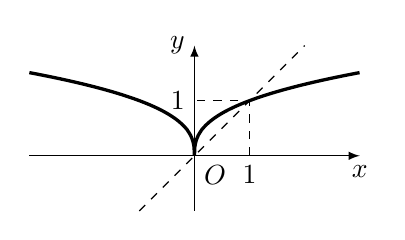
\begin{tikzpicture}[>=latex,scale = 0.7]
        \draw [->] (-3,0) -- (3,0) node [below] {$x$};
        \draw [->] (0,-1) -- (0,2) node [left] {$y$};
        \draw (0,0) node [below right] {$O$};
        \draw [dashed] (-1,-1) -- (2,2);
        \draw [domain = 0:3, samples = 400, very thick] plot (\x,{\x^(3/8)}) plot (-\x,{\x^(3/8)});
        \draw [dashed] (1,0) node [below] {$1$} -- (1,1) -- (0,1) node [left] {$1$};
    \end{tikzpicture}
\end{center}
\twoch{$p,q$均为奇数}{$p$是奇数, $q$是偶数, 且$0<\dfrac qp<1$}{$p$是偶数, $q$是奇数}{$p$是奇数, $q$是偶数, 且$\dfrac qp>1$}
\item {\tiny (002928)}已知函数$f(x)=\dfrac{x^{\frac 13}-x^{-\frac 13}}5$, $g(x)=\dfrac{x^{\frac 13}+x^{-\frac 13}}5$.\\
(1) 分别计算$f(4)-5f(2)g(2)$和$f(9)-5f(3)g(3)$的值;\\
(2) 由(1)概括出涉及函数$y=f(x)$和$y=g(x)$的, 对所有不等于零的实数$x$都成立的一个等式, 并加以证明.
\item {\tiny (002936)}若函数$f(x)=1-\sqrt{1-x^2}\ (-1\le x\le 0)$,
请画出函数$y={f^{-1}}(x)$的大致图像.
\begin{center}
    \begin{tikzpicture}[>=latex,scale =1.8]
        \foreach \i in {-1,-0.5,0,0.5,1} {\draw [dashed, gray!90] (\i,-1) -- (\i,1) (-1,\i) -- (1,\i);};
        \draw [->] (-1.5,0) -- (1.5,0) node [below] {$x$};
        \draw [->] (0,-1.5) -- (0,1.5) node [left] {$y$};
        \draw (0,0) node [below left] {$O$};
        \draw (1,0) node [below] {$1$} (0,1) node [left] {$1$};
    \end{tikzpicture}
\end{center}
\item {\tiny (002937)}已知定义在$\mathbf{R}$上的函数$y=f(x)$是奇函数, 且有反函数$y=f^{-1}(x)$. 若$a,b$是两个实数, 则下列点中, 必在$y=f^{-1}(x)$的图像上的点的序号是\blank{50}.\\
\textcircled{1} $(-f(a),a)$; \textcircled{2} $(-f(a),-a)$;\textcircled{3} $(-b,-f(b))$; \textcircled{4} $(b,-f^{-1}(-b))$.
\item {\tiny (002948)}设$a>0$, 函数$f(x)=\dfrac 1{1+a\cdot 2^x}$.\\
(1) 若$a=1$, 求$f(x)$的反函数$f^{-1}(x)$;\\
(2) 求函数$y=f(x)\cdot f(-x)$的最大值(用$a$表示);\\
(3) *设$g(x)=f(x)-f(x-1)$. 若对任意$x\in (-\infty ,0]$, $g(x)\ge g(0)$恒成立, 求$a$的取值范围.
\item {\tiny (002964)}对于函数$y=f(x)$的定义域中的任意的$x_1,x_2$($x_1\ne x_2$), 有如下结论:\\
\textcircled{1} $f(x_1+x_2)=f(x_1)\cdot f(x_2)$; \textcircled{2} $f(x_1\cdot x_2)=f(x_1)+f(x_2)$;\\ \textcircled{3} $\dfrac{f(x_1)-f(x_2)}x_1-x_2>0$; \textcircled{4} $f(\dfrac{x_1+x_2}2)<\dfrac{f(x_1)+f(x_2)}2$. 
\\当$y=\ln x$时, 上述结论中, 正确结论的序号是\blank{50}.
\item {\tiny (002965)}(1) *函数$y=\log_a|x-b|$在$(0,+\infty)$上递增, 则$a$、$b$满足\bracket{20}.
\fourch{$a>1$且$b\ge 0$}{$a>1$且$b\le 0$}{$0<a<1$且$b\ge 0$}{$0<a<1$且$b\le 0$}
(2) 函数$f(x)=\log_a|ax^2-x| \ (a>0,\ a\ne 1)$在区间$[3,4]$上是增函数, 则实数$a$的范围是\blank{50}.
\item {\tiny (002970)}*已知函数$f(x)=1+a\cdot (\dfrac 12)^x+(\dfrac 14)^x$.\\
(1) 当$a=1$时, 求函数$y=f(x)$在$(-\infty,0)$上的值域;\\
(2) 对于定义在集合$D$上的函数$y=f(x)$, 如果存在常数$M>0$, 满足: 对任意$x\in D$, 都有$|f(x)|\le M$成立, 则称$f(x)$是$D$上的有界函数, 其中$M$称为函数$f(x)$的一个上界.若函数$y=f(x)$在$[0,+\infty)$上是以$3$为一个上界的有界函数, 求实数$a$的取值范围.
\item {\tiny (002980)}已知函数$y=x+\dfrac ax$有如下性质: 如果常数$a>0$, 那么该函数在$(0, \sqrt a]$上是减函数, 在$[\sqrt a, +\infty)$上是增函数.\\
(1) 设常数$c\in [1,+\infty)$, 求函数$f(x)=x+\dfrac cx \ (1\le x\le 2)$的最大值和最小值;\\
(2) *设常数$c>0$. 当$n$是正整数时, 研究函数$g(x)=x^n+\dfrac c{x^n}$的单调性, 并说明理由.
\item {\tiny (002996)}(1) 函数$y=x^2+\dfrac 8{x^2+1}$($1\le x\le 7$)的最小值是\blank{50}, 此时$x$=\blank{50};\\
(2) 函数$y=\dfrac{3x}{x^2+4}$的值域是\blank{50};\\
(3) 函数$y=x+\dfrac m{x+3}$ , $x\in [0,+\infty)$的最小值为\blank{50};\\
(4) 设常数$m\in \mathbf{R}$. 若函数$y=\dfrac{mx}{x^2+1}$的最大值为$1$, 则$m$的值为\blank{50}.
\item {\tiny (003002)}设常数$a\in \mathbf{R}$, 区间$E\subseteq (0,+\infty)$. 已知函数$f(x)=\dfrac 1a-\dfrac 1x$, $x\in E$.\\
(1) 求证: $y=f(x)$在区间$E$上递增;\\
(2) 是否存在$a$, 使得对于这样的$a$, 总是存在 $E=[m,n]$($m<n$), 使得$y=f(x)$在区间$E$上的值域也是$E$? 若存在, 求出$a$的取值范围; 若不存在, 说明理由.
\item {\tiny (003011)}记$\max\{a_1,a_2,\cdots,a_n\}$为$a_1,\cdots,a_n$中的最大值. 已知$f(x)=\max\{x,x^2\}$($-1\le x\le 3$).\\
(1) 求函数$y=f(x)$的值域;\\
(2) 设$PAB$三点的坐标分别为$(x,f(x))$, $(0,-1)$, $(2,0)$, 且$PAB$三点可以构成三角形, 求$\triangle PAB$的面积的取值范围.
\item {\tiny (003022)}设常数$m,n\in \mathbf{R}$.已知$f(x)=(x-m)(x-n)-2$, 且$\alpha ,\beta$是方程$f(x)=0$的两个根, 则实数$m$, $n$, $\alpha$, $\beta$的大小关系可能是\bracket{20}.
\fourch{$\alpha<m<n<\beta$}{$m<\alpha<\beta<n$}{$m<\alpha<n<\beta$}{$\alpha<m<\beta<n$	}
\item {\tiny (003034)}(1) 设常数$a\in \mathbf{R}$. 已知函数$f(x)=ax$.若对于任意$x\in [-3,-1]$, 不等式$f(x)\ge 5$恒成立, 则$a$的取值范围为\blank{50};\\
(2) 设常数$a\in \mathbf{R}$. 已知函数$f(x)=ax$, 若存在$x_0\in [-3,1]$, 使得不等式$f(x)+5<0$成立, 则$a$的取值范围为\blank{50};\\
(3) 设常数$a\in \mathbf{R}$. 已知函数$f(x)=ax$. 若对于任意$x\in (-3,1)$, 不等式$f(x)+5\ge 0$恒成立, 则$a$的取值范围为\blank{50}.
\item {\tiny (003041)}已知实数$a,b$满足等式$(\dfrac 12)^a=(\dfrac 13)^b$, 下列五个关系式:\\
\textcircled{1} $0<b<a$; \textcircled{2} $a<b<0$; \textcircled{3} $0<a<b$; \textcircled{4} $b<a<0$; \textcircled{5} $a=b=0$. 其中不可能成立的关系式的序号为\blank{50}.
\item {\tiny (003043)}设常数$k\in \mathbf{R}$. 已知关于x的不等式$k\cdot 4^x-2^{x+1}+6k<0$.\\
(1) 若不等式的解集为开区间$(1, \log_2 3)$, 求$k$的取值范围;\\
(2) 若不等式对一切$x\in (1,\log_2 3)$都成立, 求$k$的取值范围;\\
(3) *若不等式的解集为开区间$(1,\log_2 3)$的子集, 求$k$的取值范围;\\
(4) *若不等式在开区间$(1,\log_2 3)$内存在解, 求$k$的取值范围.
\item {\tiny (003625)}命题$p$: 存在$a\in \mathbf{R}$且$a\ne 0$, 对任意的$x\in \mathbf{R}$, 均有$f(x+a)<f(x)+f(a)$恒成立. 已知命题$q_1$: $f(x)$单调递减, 且$f(x)>0$恒成立; 命题$q_2$: $f(x)$单调递增, 且存在${x_0}<0$使得$f({x_0})=0$. 则下列说法正确的是\bracket{20}.
\twoch{$q_1$、$q_2$都是$p$的充分条件}{只有$q_1$是$p$的充分条件}{只有$q_2$是$p$的充分条件}{$q_1$、$q_2$都不是$p$的充分条件}
\item {\tiny (003628)}在研究某市交通情况时, 道路密度是指该路段上一定时间内通过的车辆数除以时间, 车辆密度是该路段一定时间内通过的车辆数除以该路段的长度, 现定义交通流量为$v=\dfrac qx$, $x$为道路密度, $q$为车辆密度, $v=f(x)=\begin{cases} 100-135(\dfrac13)^{\frac{80}x}, & 0<x<40,  \\ -k(x-40)+85, & 40 \le x\le 80, \end{cases}$ $k>0$.\\
(1) 若交通流量$v>95$, 求道路密度$x$的取值范围; \\
(2) 若道路密度$x=80$时, 测得交通流量$v=50$, 求车辆密度$q$的最大值.
\item {\tiny (003670)}某群体的人均通勤时间, 是指单日内该群体中成员从居住地到工作地的平均用时. 某地上班族$S$中的成员仅以自驾或公交方式通勤. 分析显示: 当$S$中$x\% \ (0<x<100)$的成员自驾时, 自驾群体的人均通勤时间为
$$f(x)=\begin{cases}
30, & 0<x \le 30,\\ 2x+\dfrac{1800}{x}-90, & 30<x<100\end{cases} \ (\text{单位: 分钟}),$$
而公交群体的人均通勤时间不受$x$影响, 恒为$40$分钟. 试根据上述分析结果回答下列问题:\\
(1) 当$x$在什么范围内时, 公交群体的人均通勤时间少于自驾群体的人均通勤时间;\\
(2) 求该地上班族$S$的人均通勤时间$g(x)$的表达式; 讨论$g(x)$的单调性, 并说明其实际意义.
\item {\tiny (003693)}设定义在$\mathbf{R}$上的函数$f(x)$满足: 对于任意的$x_1,x_2\in \mathbf{R}$, 当$x_1<x_2$时, 都有$f(x_1)\le f(x_2)$.\\
(1) 若$f(x)=ax^3+1$, 求$a$的取值范围;\\
(2) 若$f(x)$是周期函数, 证明: $f(x)$是常值函数;\\
(3) 设$f(x)$恒大于零. $g(x)$是定义在$\mathbf{R}$上的、恒大于零的周期函数, $M$是$g(x)$的最大值. 函数$h(x)=f(x)g(x)$. 证明: ``$h(x)$是周期函数''的充要条件是``$f(x)$是常值函数''.
\item {\tiny (003697)}函数$f(x)=\sin x$, 对于$x_1<x_2<x_3<\cdots<x_n$且$x_1,x_2,\cdots,x_n\in [0,8\pi] \ (n\ge 10, \ n\in \mathbf{N})$, 记$M=|f(x_1)-f(x_2) |+|f(x_2)-f(x_3)|+|f(x_3)-f(x_4)|+\cdots+| f(x_{n-1})-f(x_n)|$, 则$M$的最大值等于\blank{50}.
\item {\tiny (003769)}$f(x)$是定义在$\mathbf{R}$上且周期为$2$的函数, 在区间$[-1,1]$上, $f(x)=\begin{cases}ax+1, & -1\le x<0,\\\dfrac{bx+2}{x+1}, & 0\le x\le 1,\end{cases}$ 其中$a,b\in \mathbf{R}$. 若$f\left(\dfrac 12\right)=f\left(\dfrac 32\right)$, 则$a+3b$的值为\blank{50}.
\item {\tiny (003772)}定义在$(-\infty,0)\cup (0,+\infty)$上的函数$f(x)$, 如果对于任意给定的等比数列$\{a_n\}$, $\{f(a_n)\}$仍是等比数列, 则称$f(x)$为``保等比数列函数''. 现有定义在$(-\infty,0)\cup (0,+\infty)$上的如下函数: \textcircled{1} $f(x)=x^2$; \textcircled{2} $f(x)=2^x$; \textcircled{3} $f(x)=\sqrt{|x|}$; \textcircled{4} $f(x)=\ln|x|$. 则其中是``保等比数列函数''的$f(x)$的序号为\blank{30}.
\fourch{\textcircled{1}\textcircled{2}}{\textcircled{3}\textcircled{4}}{\textcircled{1}\textcircled{3}}{\textcircled{2}\textcircled{4}}
\item {\tiny (003783)}(理科)已知$f(x)$是$\mathbf{R}$上的奇函数, $g(x)$是$\mathbf{R}$上的偶函数, 若函数$f(x)+g(x)$的值域为$[1,3)$, 则$f(x)-g(x)$的值域为\blank{50}.\\
(文科)已知$f(x)$是$\mathbf{R}$上的奇函数, $g(x)$是$\mathbf{R}$上的偶函数, 若函数$f(x)+g(x)$的值域为$[1,3)$, 则$f(-x)+g(x)$的值域为\blank{50}.
\item {\tiny (003815)}在同一坐标系中画出函数$y=\log_a x, \ y=a^x, y=x+a$的图像, 可能正确的是\blank{30}.
\fourch{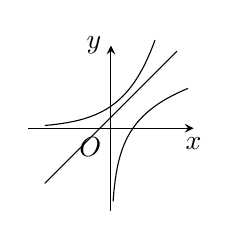
\begin{tikzpicture}[>=stealth,samples=100, scale = 0.7]
\draw [->] (-1.5,0)--(0,0) node [below left] {$O$}--(1.5,0) node [below] {$x$};
\draw [->] (0,-1.5)--(0,1.5) node [left] {$y$};
\draw [domain=-3:3] plot ({\x*0.4},{(\x+0.5)*0.4});
\draw [domain=-3:2] plot ({\x*0.4},{exp(\x*ln(2))*0.4});
\draw [domain=0.1:3.5] plot ({\x*0.4},{ln(\x)/ln(2)*0.4});
\end{tikzpicture}}{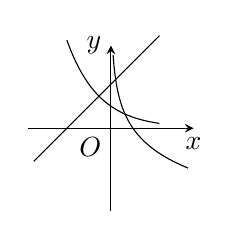
\begin{tikzpicture}[>=stealth,samples=100, scale = 0.7]
\draw [->] (-1.5,0)--(0,0) node [below left] {$O$}--(1.5,0) node [below] {$x$};
\draw [->] (0,-1.5)--(0,1.5) node [left] {$y$};
\draw [domain=-3.5:2.2] plot ({\x*0.4},{(\x+2)*0.4});
\draw [domain=-2:2.2] plot ({\x*0.4},{exp(\x*ln(1/2))*0.4});
\draw [domain=0.1:3.5] plot ({\x*0.4},{-ln(\x)/ln(2)*0.4});
\end{tikzpicture}}{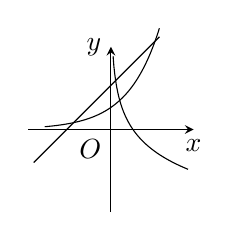
\begin{tikzpicture}[>=stealth,samples=100, scale = 0.7]
\draw [->] (-1.5,0)--(0,0) node [below left] {$O$}--(1.5,0) node [below] {$x$};
\draw [->] (0,-1.5)--(0,1.5) node [left] {$y$};
\draw [domain=-3.5:2.2] plot ({\x*0.4},{(\x+2)*0.4});
\draw [domain=-3:2.2] plot ({\x*0.4},{exp(\x*ln(2))*0.4});
\draw [domain=0.1:3.5] plot ({\x*0.4},{-ln(\x)/ln(2)*0.4});
\end{tikzpicture}}{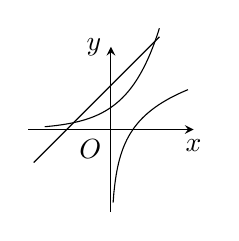
\begin{tikzpicture}[>=stealth,samples=100, scale = 0.7]
\draw [->] (-1.5,0)--(0,0) node [below left] {$O$}--(1.5,0) node [below] {$x$};
\draw [->] (0,-1.5)--(0,1.5) node [left] {$y$};
\draw [domain=-3.5:2.2] plot ({\x*0.4},{(\x+2)*0.4});
\draw [domain=-3:2.2] plot ({\x*0.4},{exp(\x*ln(2))*0.4});
\draw [domain=0.1:3.5] plot ({\x*0.4},{ln(\x)/ln(2)*0.4});
\end{tikzpicture}}
\item {\tiny (003862)}如图, 直角梯形$OABC$中, $AB\parallel OC$, $AB=1$, $OC=BC=2$, 直线$l: x=t$截此梯形所得位于$l$左方图形面积为$S$, 
\begin{center}
	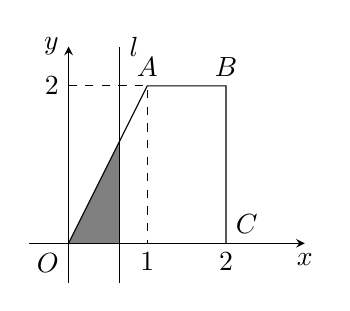
\begin{tikzpicture}[samples=200,>=stealth]
	\fill [gray] (0,0)--(0.65,0)--(0.65,1.3)--cycle;
	\draw [->] (-0.5,0)--(0,0) node [below left] {$O$} --(3,0) node [below] {$x$};
	\draw [->] (0,-0.5)--(0,2.5) node [left] {$y$};
	\draw (0,0)--(1,2) node [above] {$A$}--(2,2) node [above] {$B$}--(2,0) node [above right] {$C$};
	\draw (0.65,-0.5)--(0.65,2.5) node [right] {$l$};
	\draw [dashed] (0,2) node [left] {$2$} --(1,2)--(1,0) node [below] {$1$};
	\draw (2,0) node [below] {$2$};
	
	\end{tikzpicture}
\end{center}
则函数$S=f(t)$的图像大致为\blank{30}.
\fourch{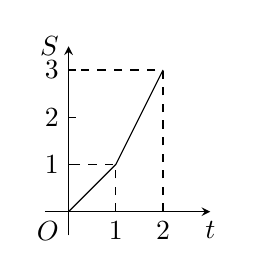
\begin{tikzpicture}[>=stealth]
	\draw [->] (-0.3,0)--(0,0) node [below left] {$O$} --(1.8,0) node [below] {$t$};
	\draw [->] (0,-0.3)--(0,2.1) node [left] {$S$};
	\draw (0.6,0) node [below] {$1$}--(0.6,0.1);
	\draw (1.2,0) node [below] {$2$}--(1.2,0.1);
	\draw (0,0.6) node [left] {$1$}--(0.1,0.6);
	\draw (0,1.2) node [left] {$2$}--(0.1,1.2);
	\draw (0,1.8) node [left] {$3$}--(0.1,1.8);
	\draw (0,0)--(0.6,0.6)--(1.2,1.8);
	\draw [dashed] (0.6,0)--(0.6,0.6)--(0,0.6);
	\draw [dashed] (1.2,0)--(1.2,1.8)--(0,1.8);
	\end{tikzpicture}}{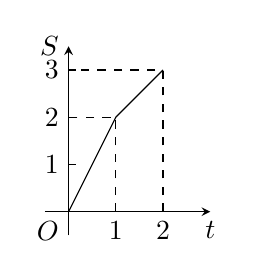
\begin{tikzpicture}[>=stealth]
	\draw [->] (-0.3,0)--(0,0) node [below left] {$O$} --(1.8,0) node [below] {$t$};
	\draw [->] (0,-0.3)--(0,2.1) node [left] {$S$};
	\draw (0.6,0) node [below] {$1$}--(0.6,0.1);
	\draw (1.2,0) node [below] {$2$}--(1.2,0.1);
	\draw (0,0.6) node [left] {$1$}--(0.1,0.6);
	\draw (0,1.2) node [left] {$2$}--(0.1,1.2);
	\draw (0,1.8) node [left] {$3$}--(0.1,1.8);
	\draw (0,0)--(0.6,1.2)--(1.2,1.8);
	\draw [dashed] (0.6,0)--(0.6,1.2)--(0,1.2);
	\draw [dashed] (1.2,0)--(1.2,1.8)--(0,1.8);
	\end{tikzpicture}}{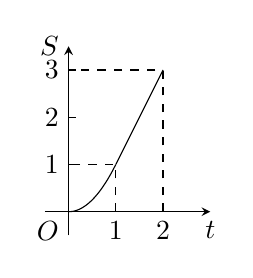
\begin{tikzpicture}[>=stealth,samples=200]
	\draw [->] (-0.3,0)--(0,0) node [below left] {$O$} --(1.8,0) node [below] {$t$};
	\draw [->] (0,-0.3)--(0,2.1) node [left] {$S$};
	\draw (0.6,0) node [below] {$1$}--(0.6,0.1);
	\draw (1.2,0) node [below] {$2$}--(1.2,0.1);
	\draw (0,0.6) node [left] {$1$}--(0.1,0.6);
	\draw (0,1.2) node [left] {$2$}--(0.1,1.2);
	\draw (0,1.8) node [left] {$3$}--(0.1,1.8);
	\draw [domain=0:1] plot ({\x*0.6},{\x*\x*0.6});
	\draw (0.6,0.6)--(1.2,1.8);
	\draw [dashed] (0.6,0)--(0.6,0.6)--(0,0.6);
	\draw [dashed] (1.2,0)--(1.2,1.8)--(0,1.8);
	\end{tikzpicture}}{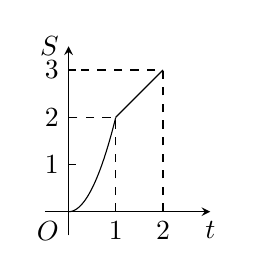
\begin{tikzpicture}[>=stealth,samples=200]
	\draw [->] (-0.3,0)--(0,0) node [below left] {$O$} --(1.8,0) node [below] {$t$};
	\draw [->] (0,-0.3)--(0,2.1) node [left] {$S$};
	\draw (0.6,0) node [below] {$1$}--(0.6,0.1);
	\draw (1.2,0) node [below] {$2$}--(1.2,0.1);
	\draw (0,0.6) node [left] {$1$}--(0.1,0.6);
	\draw (0,1.2) node [left] {$2$}--(0.1,1.2);
	\draw (0,1.8) node [left] {$3$}--(0.1,1.8);
	\draw [domain=0:1] plot ({\x*0.6},{2*\x*\x*0.6});
	\draw (0.6,1.2)--(1.2,1.8);
	\draw [dashed] (0.6,0)--(0.6,1.2)--(0,1.2);
	\draw [dashed] (1.2,0)--(1.2,1.8)--(0,1.8);
	\end{tikzpicture}}
\item {\tiny (003884)}已知函数$y=f(x)$的定义域为$\{x|-3\le x\le 8, \ x\ne 5\}$, 值域为$\{y|-1\le y\le 2, \ y\ne 0\}$. 下列关于函数$y=f(x)$的说法: \textcircled{1} 当$x=-3$时, $y=-1$; \textcircled{2} 将$y=f(x)$的图像补上$(5,0)$, 得到的图像必定是一条连续的曲线; \textcircled{3} $y=f(x)$是$[-3,5)$上的单调函数; \textcircled{4} $y=f(x)$的图像与坐标轴只有一个交点. 其中正确的命题是\blank{50}.
\item {\tiny (003892)}已知函数$f(x)$是定义在$(-\infty,0)\cup (0,+\infty)$上的偶函数, 当$x>0$时, $f(x)=\begin{cases}
2^{|x-1|}-1, & 0<x\le 2,\\\dfrac 12f(x-2), & x>2,
\end{cases}$ 则函数$g(x)=4f(x)-1$的零点的个数为\blank{30}.
\fourch{$4$}{$6$}{$8$}{$10$}
\item {\tiny (003894)}对于函数$f(x)=ax^2+(b+1)x+b-2 \ (a\ne 0)$, 若存在实数$x_0$, 使$f(x_0)=x_0$成立, 则称$x_0$为$f(x)$的不动点.\\
(1) 若对于任何实数$b$, 函数$f(x)$恒有两个相异的不动点, 求实数$a$的取值范围;\\
(2) 在(1)的条件下, 若函数$y=f(x)$的图像上$A,B$两点的横坐标是函数$f(x)$的不动点, 且直线$y=kx+\dfrac{1}{2a^2+1}$是线段$AB$的垂直平分线, 求实数$b$的取值范围.
\item {\tiny (003907)}设$f(x)$是定义在$\mathbf{R}$上的函数, 且对任意实数$x$, 恒有$f(x+2)=-3f(x)$. 当$x\in [0,2]$时, $f(x)=2x-x^2$, 则$f(0)+f(-1)+f(-2)+\cdots+f(-2014)=$\blank{30}.
\fourch{$-\dfrac 34(1-3^{1007})$}{$-\dfrac 34(1+3^{1007})$}{$-\dfrac 14\left(1-\dfrac{1}{3^{1007}}\right)$}{$-\dfrac 14\left(1+\dfrac{1}{3^{1007}}\right)$}
\item {\tiny (003921)}已知函数$f(x)=\dfrac{x}{1+|x|} \ (x\in \mathbf{R})$时, 则下列结论{\bf 不正确}的是\blank{30}.
\onech{任意$x\in \mathbf{R}$, 等式$f(-x)+f(x)=0$恒成立}{存在$m\in (0,1)$, 使得方程$|f(x)|=m$有两个不等实数根}{对任意$x_1,x_2\in \mathbf{R}$, 若$x_1\ne x_2$, 则一定有$f(x_1)\ne f(x_2)$}{存在$k\in (1,+\infty)$, 使得函数$g(x)=f(x)-kx$在$\mathbf{R}$上三个零点}
\item {\tiny (003936)}函数$y=\ln(\cos x) \ \left(-\dfrac{\pi}{2}<x<\dfrac{\pi}{2}\right)$的大致图像是\blank{30}.
\fourch{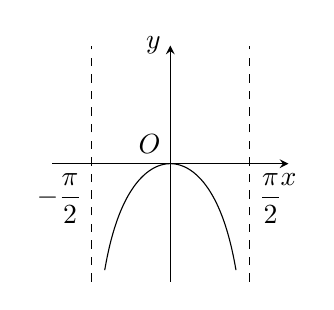
\begin{tikzpicture}[samples=200,>=stealth]
	\draw [->](-1.5,0)--(0,0) node [above left] {$O$}--(1.5,0) node [below] {$x$};
	\draw [->](0,-1.5)--(0,1.5) node [left] {$y$};
	\draw [dashed] (-1,-1.5)--(-1,1.5) (1,-1.5)--(1,1.5);
	\draw (-1,0) node [below left] {$-\dfrac{\pi}{2}$};
	\draw (1,0) node  [below right] {$\dfrac{\pi}{2}$};
	\draw [domain=-75:75] plot ({\x/90},{ln(cos(\x))});
	\end{tikzpicture}}{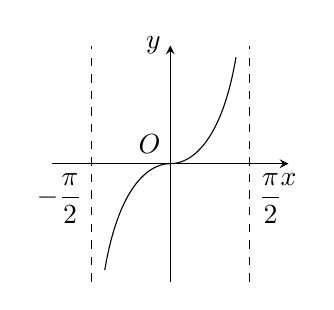
\begin{tikzpicture}[samples=200,>=stealth]
	\draw [->](-1.5,0)--(0,0) node [above left] {$O$}--(1.5,0) node [below] {$x$};
	\draw [->](0,-1.5)--(0,1.5) node [left] {$y$};
	\draw [dashed] (-1,-1.5)--(-1,1.5) (1,-1.5)--(1,1.5);
	\draw (-1,0) node [below left] {$-\dfrac{\pi}{2}$};
	\draw (1,0) node  [below right] {$\dfrac{\pi}{2}$};
	\draw [domain=-75:0] plot ({\x/90},{ln(cos(\x))});
	\draw [domain=0:75] plot ({\x/90},{-ln(cos(\x))});
	\end{tikzpicture}}{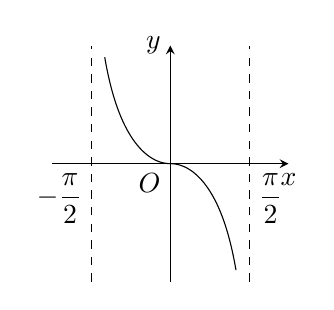
\begin{tikzpicture}[samples=200,>=stealth]
	\draw [->](-1.5,0)--(0,0) node [below left] {$O$}--(1.5,0) node [below] {$x$};
	\draw [->](0,-1.5)--(0,1.5) node [left] {$y$};
	\draw [dashed] (-1,-1.5)--(-1,1.5) (1,-1.5)--(1,1.5);
	\draw (-1,0) node [below left] {$-\dfrac{\pi}{2}$};
	\draw (1,0) node  [below right] {$\dfrac{\pi}{2}$};
	\draw [domain=-75:0] plot ({\x/90},{-ln(cos(\x))});
	\draw [domain=0:75] plot ({\x/90},{ln(cos(\x))});
	\end{tikzpicture}}{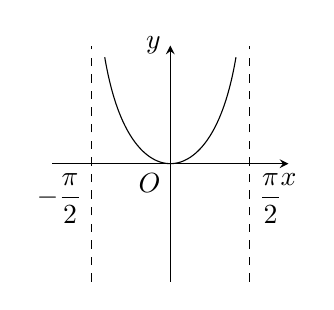
\begin{tikzpicture}[samples=200,>=stealth]
	\draw [->](-1.5,0)--(0,0) node [below left] {$O$}--(1.5,0) node [below] {$x$};
	\draw [->](0,-1.5)--(0,1.5) node [left] {$y$};
	\draw [dashed] (-1,-1.5)--(-1,1.5) (1,-1.5)--(1,1.5);
	\draw (-1,0) node [below left] {$-\dfrac{\pi}{2}$};
	\draw (1,0) node  [below right] {$\dfrac{\pi}{2}$};
	\draw [domain=-75:75] plot ({\x/90},{-ln(cos(\x))});
	\end{tikzpicture}}
\item {\tiny (003980)}(理科)在极坐标系中, ``点$P$是极点''是``点$P$的极坐标是$(0,0)$''成立的\blank{30}.
\fourch{充分不必要条件}{必要不充分条件}{充要条件}{既不充分也不必要条件}\\
(文科)$\overrightarrow a,\overrightarrow b$为非零向量, ``函数$f(x)=(x\overrightarrow a+\overrightarrow b)^2$为偶函数''是``$\overrightarrow a\perp \overrightarrow b$''的\blank{30}.
\fourch{充分不必要条件}{必要不充分条件}{充要条件}{既不充分也不必要条件}
\item {\tiny (003981)}(理科)在方程为$\begin{cases}
x=\sin 2\theta,\\ y=\sin\theta+\cos\theta
\end{cases}$的曲线上的点是\blank{30}.
\fourch{$(2,\sqrt{3})$}{$(1,\sqrt{3})$}{$\left(-\dfrac 34,\dfrac 12\right)$}{$\left(\dfrac 12,-\sqrt{2}\right)$}\\
(文科)若函数$y=f(x)$存在反函数, 则方程$f(x)=c$($c$为常数)\blank{30}.
\fourch{有且只有一个实根}{至少有一个实根}{至多有一个实根}{没有实数根}
\item {\tiny (004000)}请根据图中的函数图像, 将下列数值按从小到大的顺序排列:\blank{50}.
\begin{center}
    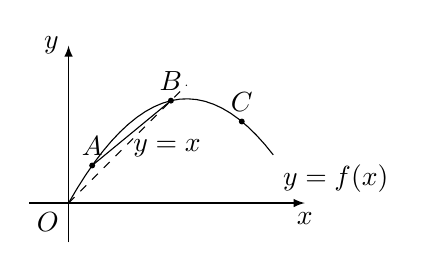
\begin{tikzpicture}[>=latex]
        \draw [->] (-0.5,0) -- (3,0) node [below] {$x$};
        \draw [->] (0,-0.5) -- (0,2) node [left] {$y$};
        \draw (0,0) node [below left] {$O$};
        \draw [domain = 0:2.6, name path = curve] plot (\x,{\x*(3-\x)/1.7}) node [below right] {$y=f(x)$};
        \draw [dashed] (0,0) -- (1.5,1.5);
        \filldraw (1.3,1.3) circle (0.03) node [above] {$B$} -- (0.3,{0.3*2.7/1.7}) circle (0.03) node [above] {$A$};
        \filldraw (2.2,{2.2*0.8/1.7}) circle (0.03) node [above] {$C$};
        \draw (0.7,0.7) node [right] {$y=x$};
    \end{tikzpicture}    
\end{center}
\textcircled{1} 曲线在点$A$处切线的斜率;\\
\textcircled{2} 曲线在点$B$处切线的斜率;\\
\textcircled{3} 曲线在点$C$处切线的斜率;\\
\textcircled{4} 割线$AB$的斜率;\\
\textcircled{5} 数值$0$;\\
\textcircled{6} 数值$1$.
\item {\tiny (004007)}已知$y=f'(x)$的图像如图所示, 求函数$y=f(x)$在$(-2,2)$上的单调区间和极值点.
\begin{center}
    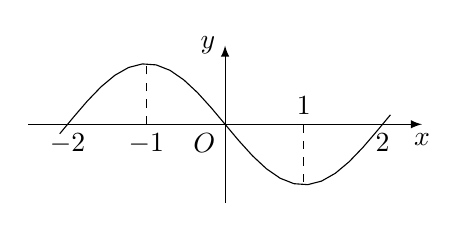
\begin{tikzpicture}[>=latex]
        \draw [->] (-2.5,0) -- (2.5,0) node [below] {$x$};
        \draw [->] (0,-1) -- (0,1) node [left] {$y$};
        \draw (0,0) node [below left] {$O$};
        \draw [domain = -2.1:2.1] plot (\x, {-sin(\x*90)/1.3});
        \draw [dashed] (-1,0) node [below] {$-1$} -- (-1,{1/1.3}) (1,0) node [above] {$1$}-- (1,{-1/1.3});
        \draw (-2,0) node [below] {$-2$} (2,0) node [below] {$2$};
    \end{tikzpicture}
\end{center}
\item {\tiny (004067)}已知定义在$\mathbf{R}$上的函数$f(x)$满足: \textcircled{1} $f(x)+f(2-x)=0$; \textcircled{2} $f(x)-f(-2-x)=0$; \textcircled{3} 在$[-1,1]$上表达式为$f(x)=\begin{cases} \sqrt{1-x^2}, & x\in [-1,0], \\ 1-x, & x\in (0,1], \end{cases}$ 则函数$f(x)$与$g(x)=\begin{cases} {2^x}, & x\le 0 \\ \log_\frac 12x, & x>0 \end{cases}$的图像在区间$[-3,3]$上的交点的个数为\blank{50}.
\item {\tiny (004074)}如图, 在直角坐标平面内有一个边长为$a$, 中心在原点$O$的
正六边形$ABCDEF$, $AB\parallel Ox$. 直线$l:y=kx+t$ ($k$是常数)与正六边形交于$M$、$N$两点, 记$\triangle OMN$的面积为$S$, 则函数$S=f(t)$的奇偶性为\bracket{20}.
\begin{center}
    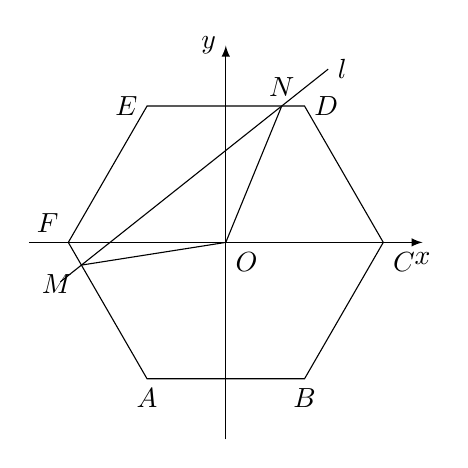
\begin{tikzpicture}[>=latex]
        \draw [->] (-2.5,0) -- (2.5,0) node [below] {$x$};
        \draw [->] (0,-2.5) -- (0,2.5) node [left] {$y$};
        \draw (0,0) node [below right] {$O$};
        \draw [name path = hexagon] (-1,{-sqrt(3)}) node [below] {$A$} -- (1,{-sqrt(3)}) node [below] {$B$} -- (2,0) node [below right] {$C$} -- (1,{sqrt(3)}) node [right] {$D$} -- (-1,{sqrt(3)}) node [left] {$E$} -- (-2,0) node [above left] {$F$} -- cycle;
        \draw [name path = linel] (-2.1,-0.5) -- (1.3,2.2)node [right] {$l$};
        \path [name intersections = {of = hexagon and linel, by = {N,M}}];
        \draw (N) node [above] {$N$} -- (0,0) -- (M) node [below left] {$M$};
    \end{tikzpicture}
\end{center}
\twoch{偶函数}{奇函数}{不是奇函数, 也不是偶函数}{奇偶性与$k$有关}
\item {\tiny (004079)}已知函数$f(x)=\log_2x$.\\
(1) 若$f(x)$的反函数是$f^{-1}(x)$, 解方程: $f^{-1}(2x+1)=3f^{-1}(x)-1$;\\
(2) 当$x\in (3m, 3m+3]$($m\in \mathbf{N}$)时, 定义$g(x)=f(x-3m)$. 设$a_n=n\cdot g(n)$, 数列$\{a_n\}$ 的前$n$项和为$S_n$, 求$a_1$、$a_2$、$a_3$、$a_4$和$S_{3n}$;\\
(3) 对于任意$a$、$b$、$c\in [M,+\infty)$, 且$a\ge b\ge c$. 当$a$、$b$、$c$能作为一个三角形的三边长时, $f(a)$、$f(b)$、$f(c)$也总能作为某个三角形的三边长, 试探究$M$的最小值.
\item {\tiny (004090)}在直角$\triangle ABC$中, $\angle A=\dfrac{\pi}2$, $AB=1$, $AC=2$, $M$是$\triangle ABC$内一点, 且$AM=\dfrac 12$, 若$\overrightarrow{AM}=\lambda \overrightarrow{AB}+\mu \overrightarrow{AC}$, 则$\lambda +2\mu$的最大值为\blank{50}.
\item {\tiny (004094)}已知$f(x)$是定义在$\mathbf{R}$上的奇函数, 对任意两个不相等的正数$x_1$, $x_2$都有$\dfrac{x_2f(x_1)-x_1f(x_2)}{x_1-x_2}<0$, 则函数$g(x)=\begin{cases} \dfrac{f(x)}x, &x\ne 0, \\ 0, & x=0 \end{cases}$\bracket{20}.
\twoch{是偶函数, 且在$(0,+\infty)$上单调递减}{是偶函数, 且在$(0,+\infty)$上单调递增}{是奇函数, 且单调递减}{是奇函数, 且单调递增}
\item {\tiny (004116)}已知集合$M=\{(x,y)|y=f(x)\}$, 若对于任意$(x_1,y_1)\in M$, 存在$(x_2,y_2)\in M$, 使得$x_1x_2+y_1y_2=0$成立, 则称集合$M$是``$\Omega$集合''. 给出下列$4$个集合:
\textcircled{1} $M=\{(x,y) |y=\dfrac 1x \}$; \textcircled{2} $M=\{(x,y)|y=\mathrm{e}^x-2\}$; \textcircled{3} $M=\{(x,y)|y=\cos x\}$; \textcircled{4} $M=\{(x,y)|y=\ln x\}$.
其中所有``$\Omega$集合''的序号是\bracket{20}.
\fourch{\textcircled{2}\textcircled{3}}{\textcircled{3}\textcircled{4}}{\textcircled{1}\textcircled{2}\textcircled{4}}{\textcircled{1}\textcircled{3}\textcircled{4}}
\item {\tiny (004157)}已知函数$f(x)=x+\dfrac ax$($a>0$), $0<x_1<x_2$, 且$f(x_1)=f(x_2)$, 给出以下结论:\\
\textcircled{1} $\dfrac{x_1+x_2}2>\sqrt a$恒成立; \textcircled{2} $f(2\sqrt a-x_1)<f(x_2)$恒成立. 则\bracket{20}.
\fourch{\textcircled{1}正确, \textcircled{2}正确}{\textcircled{1}正确, \textcircled{2}错误}{\textcircled{1}错误, \textcircled{2}正确}{\textcircled{1}错误, \textcircled{2}错误}
\item {\tiny (004161)}某学校对面有一块空地要围建成一个面积为$360\text{m}^2$的矩形场地, 要求矩形场地的一面利用旧墙(旧墙需要整修), 其它三面围墙要新建, 在旧墙对面的新墙上要留一个宽度为$2\text{m}$的进出口, 如图所示. 已知旧墙的整修费用为$45\text{元/m}$, 新建墙的造价为$180\text{元/m}$, 建$2\text{m}$宽的进出口需$2360$元的单独费用, 设利用的旧墙的长度为$x$(单位: $\text{m}$), 设修建此矩形场地围墙的总费用(含建进出口的费用)为$y$(单位: 元).\\
\begin{center}
    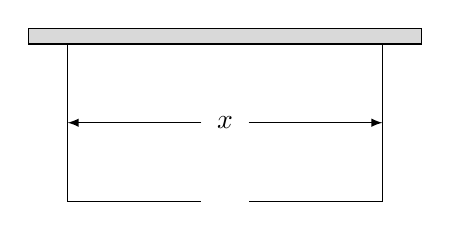
\begin{tikzpicture}[>=latex]
        \filldraw [gray!30] (0,0) rectangle (5,0.2);
        \draw (0,0) rectangle (5,0.2);
        \draw (0.5,0) -- (0.5,-2) -- (2.2,-2) (4.5,0) -- (4.5,-2) -- (2.8,-2);
        \draw (2.5,-1) node {$x$};
        \draw [->] (2.2,-1) -- (0.5,-1);
        \draw [->] (2.8,-1) -- (4.5,-1); 
    \end{tikzpicture}
\end{center}
(1) 将$y$表示为$x$的函数;\\
(2) 试确定$x$, 使修建此矩形场地围墙的总费用(含建进出口的费用)最少, 并求出最少总费用.
\item {\tiny (004184)}设$m$为给定的实常数, 若函数$y=f(x)$在其定义域内存在实数$x_0$, 使得$f(x_0+m)=f(x_0)+f(m)$成立, 则称函数$f(x)$为``$G(m)$函数''.\\
(1) 若函数$f(x)=2^x$为``$G(2)$函数'', 求实数$x_0$的值;\\
(2) 若函数$f(x)=\lg \dfrac a{x^2+1}$为``$G(1)$函数'', 求实数$a$的取值范围;\\
(3) 已知$f(x)=x+b$($b\in \mathbf{R}$)为``$G(0)$函数'', 设$g(x)=x|x-4|$. 若对任意的$x_1,x_2\in[0,t]$, 当$x_1\ne x_2$时, 都有$\dfrac{g(x_1)-g(x_2)}{f(x_1)-f(x_2)}>2$成立, 求实数$t$的最大值.
\item {\tiny (004203)}已知函数$f(x)=ax+\log_2(2^x+1)$, 其中$a\in \mathbf{R}$.\\
(1) 根据$a$的不同取值, 讨论$f(x)$的奇偶性, 并说明理由;\\
(2) 已知$a>0$, 函数$f(x)$的反函数为$f^{-1}(x)$, 若函数$y=f(x)+f^{-1}(x)$在区间$[1,2]$上的最小值为$1+\log_23$, 求函数$f(x)$在区间$[1,2]$上的最大值.
\item {\tiny (004220)}已知函数\textcircled{1} $f(x)=3\ln x$; \textcircled{2} $f(x)=3\mathrm{e}^{\cos x}$; \textcircled{3} $f(x)=3\mathrm{e}^x$; \textcircled{4} $f(x)=3\cos x$; 其中对于$f(x)$定义域内的任意一个自变量$x_1$都存在唯一一个自变量$x_2$, 使$\sqrt{f(x_1)f(x_2)}=3$成立的函数是\bracket{20}.
\fourch{\textcircled{3}}{\textcircled{2}\textcircled{3}}{\textcircled{1}\textcircled{2}\textcircled{4}}{\textcircled{4}}
\item {\tiny (004224)}对于两个定义域相同的函数$f(x)$、$g(x)$, 若存在实数$m$、$n$, 使$h(x)=mf(x)+ng(x)$, 则称函数$h(x)$是由``基函数$f(x)$、$g(x)$''生成的.\\
(1) $f(x)=x^2+3x$和$g(x)=3x+4$生成一个偶函数$h(x)$, 求$h(2)$的值;\\
(2) 若$h(x)=2x^2+3x-1$由$f(x)=x^2+ax$, $g(x)=x+b$($a,b\in \mathbf{R}$且$ab\ne 0$)生成, 求$a+2b$的取值范围.
\item {\tiny (004238)}对实数$x\in \mathbf{R}$, 函数$f(x)$满足: $f(x+1)=\sqrt{f(x)-{f^2}(x)}+\dfrac 12$, $a_n=f^2(n)-f(n)$,
数列$\{a_n\}$的前$15$项和为$-\dfrac{31}{16}$, 数列$\{c_n\}$满足$c_n+c_{n+1}=[f(2019)]^n$, 若数列$\{c_n\}$的前$n$项和$S_n$的极限存在, 则$c_1=$\blank{50}.
\item {\tiny (004247)}设函数$f(x)$在$[1,+\infty)$上有定义, 实数$a$和$b$满足$1\le a<b$, 若$f(x)$在区间$(a,b]$上不存在最小值, 则称$f(x)$在区间$(a,b]$上具有性质$P$.\\
(1) 当$f(x)=x^2+cx$, 且$f(x)$在区间$(1,2]$上具有性质$P$, 求实数$c$的取值范围;\\
(2) 已知$f(x+1)=f(x)+1$($x\ge 1$), 且当$1\le x<2$时, $f(x)=1-x$, 判别$f(x)$在区间$(1,4]$ 上是否具有性质$P$;\\
(3) 若对于满足$1\le a<b$的任意实数$a$和$b$, $f(x)$在区间$(a,b]$上具有性质$P$, 且对于任意$n\in \mathbf{N}^*$, 当$x\in (n,n+1)$时, 有$|f(n)-f(x)|+|f(x)-f(n+1)|=|f(n)-f(n+1)|$, 证明: 当$x\ge 1$时, $f(2x)>f(x)$.
\item {\tiny (004259)}已知定义在$\mathbf{R}$上的函数$f(x)$满足$f(x+1)=2f(x)+1$, 当$x\in [0,1)$时, $f(x)=x^3$. 设$f(x)$在区间$[n,n+1)$($n\in \mathbf{N}^*$)上的最小值为$a_n$, 若存在$n\in \mathbf{N}^*$, 使得$\lambda (a_n+1)<2n-7$成立, 则实数$\lambda$的取值范围是\blank{50}.
\item {\tiny (004284)}已知函数$f(x)=m\cdot 2^x+x^2+nx$, 记集合$A=\{x|f(x)=0, \ x\in \mathbf{R}\}$, 集合$B=\{x|f(f(x))=0, \ x\in \mathbf{R}\}$.
若$A=B$, 且$A$、$B$都不是空集, 则$m+n$的取值范围是\bracket{20}.
\fourch{$[0,4)$}{$[-1,4)$}{$[-3,5]$}{$[0,7)$}
\item {\tiny (004305)}定义$F(a,b)=\begin{cases} a, & a \le b, \\ b, & a>b,\end{cases}$, 已知函数$f(x)$、$g(x)$定义域都是$\mathbf{R}$, 给出下列命题:\\
(1) 若$f(x)$、$g(x)$都是奇函数, 则函数$F(f(x),g(x))$为奇函数;\\
(2) 若$f(x)$、$g(x)$都是减函数, 则函数$F(f(x),g(x))$为减函数;\\
(3) 若$f_{\min}(x)=m$, $g_{\min}(x)=n$, 则$F_{\min}(f(x),g(x))=F(m,n)$;\\
(4) 若$f(x)$、$g(x)$都是周期函数, 则函数$F(f(x),g(x))$是周期函数.\\
其中正确命题的个数为\bracket{20}.
\fourch{$1$个}{$2$个}{$3$个}{$4$个}
\item {\tiny (004328)}经济订货批量模型, 是目前大多数工厂、企业等最常采用的订货方式, 即某种物资在单位时间的需求量为某常数, 经过某段时间后, 存储量消耗下降到零, 此时开始订货并随即到货, 然后开始下一个存储周期. 该模型适用于整批间隔进货、不允许缺货的存储问题. 具体如下:\\
年存储成本费$T$(元)关于每次订货$x$(单位: 吨)的函数关系为$T(x)=\dfrac{Bx}2+\dfrac{AC}x$, 其中$A$为年需求量, $B$为每单位物资的年存储费, $C$为每次订货费.\\
某化工厂需用甲醇作为原料, 年需求量为$6000$吨, 每吨存储费为$120$元/年, 每次订货费为$2500$元.
(1) 若该化工厂每次订购$300$吨甲醇, 求年存储成本费;\\
(2) 每次需订购多少吨甲醇, 可使该化工厂年存储成本费最少? 最少费用为多少?
\item {\tiny (004373)}已知函数$f(x)=x|x-a|$, 其中$a$为常数.\\
(1) 当$a=1$时, 解不等式$f(x)<2$;\\
(2) 已知$g(x)$是以$2$为周期的偶函数, 且当$0\le x\le 1$时, 有$g(x)=f(x)$. 若$a<0$, 且$g(\dfrac 32)=\dfrac 54$, 求函数$y=g(x)$($x\in [1,2]$)的反函数;\\
(3) 若在$[0,2]$上存在$n$个不同的点$x_i$($i=1,2,\cdots,n$, $n\ge 3$), $x_1<x_2<\cdots <x_n$, 使得$|f(x_1)-f(x_2)|+|f(x_2)-f(x_3)|+\cdots+|f(x_{n-1})-f(x_n)|=8$, 求实数$a$的取值范围.
\item {\tiny (004387)}设函数$f(x)$的定义域为$(0,+\infty)$, 若对任意$x\in (0,+\infty)$, 恒有$f(2x)=2f(x)$, 则称$f(x)$为``$2$阶缩放函数''.\\
(1) 已知函数$f(x)$为``$2$阶缩放函数'', 当$x\in (1,2]$时, $f(x)=1-\log_2 x$, 求$f(2\sqrt{2})$的值;\\
(2) 已知函数$f(x)$为``$2$阶缩放函数'', 当$x\in (1,2]$时, $f(x)=\sqrt{2x-x^2}$, 求证: 函数$y=f(x)-x$在$(1,+\infty)$上无零点.
\item {\tiny (004399)}对于全集$\mathbf{R}$的子集$A$, 定义函数$f_A(x)=\begin{cases}
1, &  x\in A,  \\0, & x\in \complement_{\mathbf{R}}A  \end{cases}$为$A$的特征函数, 设$A,B$为全集$\mathbf{R}$的子集,\\
\textcircled{1} 若$A\subseteq B$, 则$f_A(x)\le f_B(x)$; \textcircled{2} $f_{\complement_{\mathbf{R}}A}(x)=1-f_A(x)$;\\
\textcircled{3} ${f_{A\cap B}}(x)=f_A(x)\cdot f_B(x)$; \textcircled{4} $f_{A\cup B}(x)=f_A(x)+f_B(x)$;\\ \textcircled{5} $f_{A\cap \complement_\mathbf{R}B}(x)=f_A(x)-f_B(x)$; \textcircled{6} 对于任意$x\in \mathbf{R}$, 若$f_A(x)\cdot f_B(x)=0$恒成立, 则$A\cap B=\varnothing$.\\
其中正确的命题为\blank{50}(填所有正确命题的序号).
\item {\tiny (004407)}已知函数$f(x)=\dfrac{ax^2+1}{bx+c}$是奇函数, $a,b,c$为常数.\\
(1)	求实数$c$的值;\\
(2)	若$a,b\in \mathbf{Z}$, 且$f(1)=2$, $f(2)<3$, 求$f(x)$的解析式;\\
(3) 已知$b>0$, 若$f(x)\ge f(1)$在$(0,+\infty)$上恒成立, 且$\{x|f[f(x)]\ge x\}\cap [1,2]\ne \varnothing$, 求$b$的取值范围.
\item {\tiny (004424)}设$\mu (x)$表示不小于$x$的最小整数, 例如$\mu(0.3)=1$, $\mu(-2.5)=2$.\\
(1) 解方程$\mu(x-1)=3$;\\
(2) 设$f(x)=\mu (x\cdot \mu (x))$, $n\in \mathbf{N}^*$, 试分别求出$f(x)$在区间$(0,1]$、$(1,2]$以及$(2,3]$上的值域; 若$f(x)$在区间$(0,n]$上的值域为$M_n$, 求集合$M_n$中的元素的个数;\\
(3) 设实数$a>0$, $g(x)=x+a\cdot \dfrac{\mu (x)}x-2$, $h(x)=\dfrac{\sin (\pi x)+2}{x^2-5x+7}$, 若对于任意$x_1,x_2\in (2,4]$都有$g(x_1)>h(x_2)$, 求实数$a$的取值范围.
\item {\tiny (004440)}已知函数$f(x)=\begin{cases}\log_{\frac 12}(1-x), & -1\le x\le n,  \\ 2^{2-|x-1|}-3, & n<x\le m,  \end{cases}$($n<m$)的值域是$[-1,1]$, 有下列结论:
\textcircled{1} 当$n=0$时, $m$的取值范围为$(0,2]$; \textcircled{2}  当$n=\dfrac 12$时, $m$的取值范围为$(\dfrac 12,2]$; \textcircled{3}  当$n\in [0,\dfrac 12)$时, $m$的取值范围为$[1,2]$; \textcircled{4}  当$n\in [0,\dfrac 12)$时, $m$的取值范围为$(n,2]$;
其中结论正确的所有的序号是\bracket{20}.
\fourch{\textcircled{1}\textcircled{2}}{\textcircled{3}\textcircled{4}}{\textcircled{2}\textcircled{3}}{\textcircled{2}\textcircled{4}}
\item {\tiny (004444)}定义区间$(m,n)$、$[m,n]$、$(m,n]$、$[m,n)$的长度均为$n-m$, 已知不等式$\dfrac 7{6-x}\ge 1$的解集为$A$.\\
(1) 求$A$的长度;\\
(2) 函数$f(x)=\dfrac{(a^2+a)x-1}{a^2x}$($a\in \mathbf{R}$, $a\ne 0$)的定义域与值域都是$[m,n]$($n>m$), 求区间$[m,n]$的最大长度;\\
(3) 关于$x$的不等式$\log_2x+\log_2(tx+3t)<2$的解集为$B$, 若$A\cap B$的长度为$6$, 求实数$t$的取值范围.
\item {\tiny (004463)}《上海市生活垃圾管理条例》于$2019$年$7$月$1$日正式实施. 某小区全面实施垃圾分类处理. 已知该小区每月垃圾分类处理量不超过$300$吨, 每月垃圾分类处理成本$y$(元)与每月分类处理量$x$(吨)之间的函数关系式可近似表示为
$y=x^2-200x+40000$,而分类处理一吨垃圾小区也可以获得$300$元的收益.\\
(1) 该小区每月分类处理多少吨垃圾, 才能使得每吨垃圾分类处理的平均成本最低?\\
(2) 要保证该小区每月的垃圾分类处理不亏损, 每月的垃圾分类处理量应控制在什么范围?
\item {\tiny (004483)}如图, 正方形$OABC$的边长为$a$($a>1$), 函数$y=3x^2$交$AB$于点$Q$, 函数$y=x^{-\frac 12}$与$BC$交于点$P$, 当$|AQ|+|CP|$最小时, $a$的值为\blank{50}.
\begin{center}
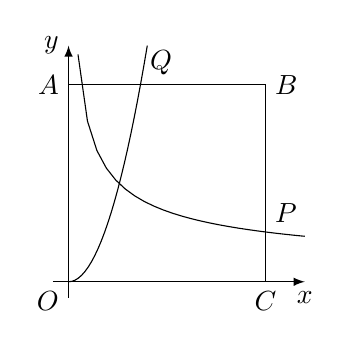
\begin{tikzpicture}[>=latex]
\draw [->] (-0.2,0) -- (3,0) node [below] {$x$};
\draw [->] (0,-0.2) -- (0,3) node [left] {$y$};
\draw (0,0) node [below left] {$O$};
\draw (2.5,0) node [below] {$C$} coordinate (C);
\draw (2.5,2.5) node [right] {$B$} coordinate (B);
\draw (0,2.5) node [left] {$A$} coordinate (A);
\draw [domain = 0:1] plot (\x,{3*\x*\x});
\draw [domain = 0.12:3] plot (\x,{pow(\x,-1/2)});
\draw (C) -- (B) -- (A);
\draw ({sqrt(2.5/3)},2.5) node [above right] {$Q$};
\draw (2.5,{pow(2.5,-1/2)}) node [above right] {$P$};
\end{tikzpicture}
\end{center}
\item {\tiny (004486)}某温室大棚规定: 一天中, 从中午$12$点到第二天上午$8$点为保温时段, 其余$4$小时为工人作业时段. 从中午$12$点连续测量$20$小时, 得出此温室大棚的温度$y$(单位: 度)与时间$t$(单位: 小时, $t\in [0,20]$)近似地满足函数$y=|t-13|+\dfrac b{t+2}$关系, 其中, $b$为大棚内一天中保温时段的通风量.\\
(1) 若一天中保温时段的通风量保持$100$个单位不变, 求大棚一天中保温时段的最低温度(精确到$0.1^\circ\text{C}$);\\
(2) 若要保持大棚一天中保温时段的最低温度不小于$17^\circ\text{C}$, 求大棚一天中保温时段通风量的最小值.
\item {\tiny (004525)}已知函数$f(x)=\begin{cases} x^2, & x\text{为无理数}, \\ x, &x\text{为有理数},   \end{cases}$ 则以下$4$个命题:
\textcircled{1} $f(x)$是偶函数; \textcircled{2} $f(x)$在$[0,+\infty)$上是增函数; \textcircled{3} $f(x)$的值域为$\mathbf{R}$; \textcircled{4} 对于任意的正有理数$a$, $g(x)=f(x)-a$存在奇数个零点.
其中正确命题的个数为\bracket{20}.
\fourch{$0$}{$1$}{$2$}{$3$}
\item {\tiny (004546)}若直线$y=kx+1$与曲线$y=|x+\dfrac 1x|-|x-\dfrac 1x|$有且仅有四个不同的交点, 则实数$k$的取值范围为\bracket{20}.
\fourch{$\{-\dfrac 18,0,\dfrac 18\}$}{$\{-\dfrac 18,\dfrac 18\}$}{$[-\dfrac 18,\dfrac 18]$}{$(-\dfrac 18,\dfrac 18)$}
\item {\tiny (004549)}某省4A级风景区内居住着一个少数民族村, 该村投资了$800$万元修复和加强民俗文化基础设施. 据调查, 修复好村民俗文化基础设施后, 任何一个月内(每月按$30$天计)每天的旅游人数$f(x)$与第$x$天近似地满足$f(x)=8+\dfrac 9x$(千人), 且参观民俗文化村的游客人均消费$g(x)$近似地满足$g(x)=143-|x-22|$(元).\\
(1) 求该村第$x$天的旅游收入$p(x)$(单位千元, $1\le x\le 30,x\in \mathbf{N}^*$)的函数关系;\\
(2) 若以最低日收入的$20\%$作为每一天的纯收入的计量依据, 并以纯收入的$5\%$的比例收回投资成本, 试问该村在两年内能否收回全部投资成本?
\item {\tiny (004569)}改革开放$40$年, 我国卫生事业取得巨大成就, 卫生总费用增长了数十倍. 卫生总费用包括个人现在支出、社会支出、政府支出, 如表为$2012$年至$2015$年我国卫生费用中个人现金支出、社会支出和政府支出的费用(单位:亿元)和在卫生总费用中的占比. 
\begin{center}
    \begin{tabular}{|p{.05\textwidth}<\centering|p{.1\textwidth}<\centering|p{.1\textwidth}<\centering|p{.1\textwidth}<\centering|p{.1\textwidth}<\centering|p{.1\textwidth}<\centering|p{.1\textwidth}<\centering|p{.1\textwidth}<\centering|}
        \hline
         & & \multicolumn{2}{c|}{个人现金卫生支出} & \multicolumn{2}{c|}{社会卫生支出} & \multicolumn{2}{c|}{政府卫生支出} \\ \hline
         年份& 卫生总费用(亿元)& 绝对数(亿元) & 占卫生总费用比重($\%$) & 绝对数(亿元) & 占卫生总费用比重($\%$)& 绝对数(亿元) & 占卫生总费用比重($\%$)\\ \hline
        $2012$ & $28119.00$ & $9656.32$ & $34.34$ & $10030.70$ & $35.67$ & $8431.98$ & $29.99$ \\ \hline
        $2013$ & $31668.95$ & $10729.34$ & $33.88$ & $11393.79$ & $35.98$ & $9545.81$ & $30.14$ \\ \hline
        $2014$ & $35312.40$ & $11295.41$ & $31.99$ & $13437.75$ & $38.05$ & $10579.23$ & $29.96$ \\ \hline
        $2015$ & $40974.64$ & $11992.65$ & $29.27$ & $16506.71$ & $40.29$ & $12475.28$ & $30.45$ \\ \hline
    \end{tabular}
\end{center}
(数据来源于国家统计年鉴)\\
(1) 指出$2012$年到$2015$年之间我国卫生总费用中个人现金支出占比和社会支出占比的变化趋势;\\
(2) 设$t=1$表示$1978$年, 第$t$年卫生总费用与年份$t$之间拟合函数$f(t)=\dfrac{357876.6053}{1+\mathrm{e}^{6.4420-0.1136t}}$, 研究函数$f(t)$的单调性, 并预测我国卫生总费用首次超过$12$万亿的年份.
\item {\tiny (004679)}为实现``碳达峰'', 减少污染, 某化工企业开发了一个废料回收项目. 经测算, 该项目日回收成本$p$(元)与日回收量$x$(吨)($x\in [0,50]$)的函数关系可表示为$p=\begin{cases}20x, & 0\le x\le 30,  \\ x^2+16x-780, & 30<x \le 50,  \end{cases}$ 且每回收$1$吨废料, 转化成其他产品可收入$80$元.\\
(1) 设日纯收益为$y$元, 写出函数$y=f(x)$的解析式(纯收益$=$收入$-$成本);\\
(2) 该公司每日回收废料多少吨时, 获得纯收益最大?
\item {\tiny (004721)}如图, 有一块扇形草地$OMN$, 已知半径为$4$, $\angle MON=\dfrac\pi 2$, 现要在其中圈出一块举行场地$ABCD$作为儿童乐园使用, 其中点$A$、$B$在弧$\overset\frown{MN}$上, 且线段$AB$平行于线段$MN$.
\begin{center}
    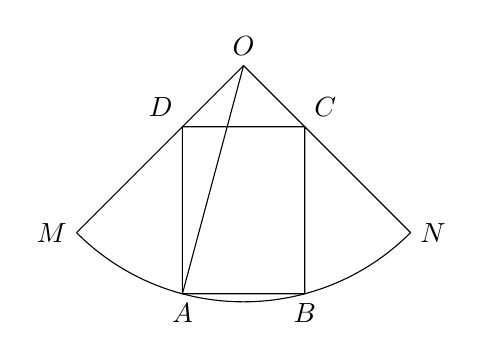
\begin{tikzpicture}[scale = 1.5]
        \draw (0,0) node [above] {$O$} coordinate (O);
        \draw (-45:2) node [right] {$N$} coordinate (N);
        \draw (-135:2) node [left] {$M$} coordinate (M);
        \draw (-75:2) node [below] {$B$} coordinate (B);
        \draw (-105:2) node [below] {$A$} coordinate (A);
        \draw (-45:{2/sin(45)*sin(15)}) node [above right] {$C$} coordinate (C);
        \draw (-135:{2/sin(45)*sin(15)}) node [above left] {$D$} coordinate (D);
        \draw (M) -- (O) -- (N) (A) rectangle (C) (O) -- (A);
        \draw (M) arc (-135:-45:2);
    \end{tikzpicture}
\end{center}
(1) 若点$A$为弧$\overset\frown{MN}$的一个三等分点, 求矩形$ABCD$的面积$S$;\\
(2) 当$A$在何处时, 矩形$ABCD$的面积$S$最大? 最大值为多少?
\item {\tiny (004760)}已知以下三个陈述句:\\
$p$: 存在$a\in \mathbf{R}$且$a\ne 0$, 对任意的$x\in \mathbf{R}$, 均有$f(2^{x+a})<f(2^x)+f(a)$恒成立;\\
$q_1$: 函数$y=f(x)$是定义域为$\mathbf{R}$的减函数, 且对任意的$x\in \mathbf{R}$, 都有$f(x)>0$;\\
$q_2$: 函数$y=f(x)$是定义域为$\mathbf{R}$的增函数, 存在$x_0<0$, 使得$f(x_0)=0$;\\
用这三个陈述句组成两个命题, 命题$S$: ``若$q_1$, 则$p$''; 命题$T$: ``若$q_2$, 则$p$''. 关于$S,T$以下说法正确的是\bracket{20}.
\twoch{只有命题$S$是真命题}{只有命题$T$是真命题}{两个命题$S,T$都是真命题}{两个命题$S,T$都不是真命题}
\item {\tiny (004763)}新冠肺炎疫情造成医用防护服紧缺, 某地政府决定为防护服生产企业A公司扩大生产提供$x$($x\in [0,10]$)(万元)的专项补贴, 并以每套$80$元的价格收购其生产的全部防护服. $A$公司在收到政府$x$(万元)补贴后, 防护服产量将增加到$t=k\cdot (6-\dfrac{12}{x+4})$(万套), 其中$k$为工厂工人的复工率($k\in [0.5,1]$). $A$公司生产$t$万件防护服还需投入成本$20+8x+50t$(万元).\\
(1) 将$A$公司生产防护服的利润$y$(万元)表示为补贴$x$(万元)的函数(利润不包含政府补贴);\\
(2) 若对任意的$x\in [0,10]$(万元), $A$公司都不会产生亏损, 求复工率$k$的取值范围.
\item {\tiny (005136)}在$\triangle ABC$中, 已知$BC=a$, $CA=b$, $AB=c$, $\angle ACB=\theta$. 现将$\triangle ABC$分别以$BC,CA,AB$所在直线为轴旋转一周, 设所得三个旋转体的体积依次为$V_1,V_2,V_3$.\\
(1) 设$T=\dfrac{V_3}{V_1+V_2}$, 试用$a,b,c$表示$T$;\\
(2) 若$\theta$为定值, 并令$\dfrac{a+b}c=x$, 将$T=\dfrac{V_3}{V_1+V_2}$表示为$x$的函数, 写出这个函数的定义域, 并求这个函数的最大值$M$;\\
(3) 若$\theta \in [\dfrac{\pi }3,\pi)$, 求(2)中$M$的最大值.
\item {\tiny (005284)}集合$M=\{a,b,c\}$与$P=\{x,y,z\}$之间建立起四种对应关系(如图), 则下列结论中正确的是\bracket{20}.
\begin{center}
    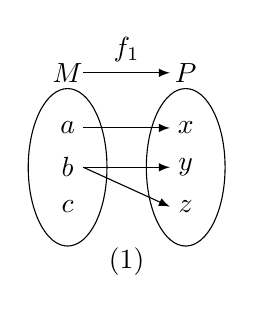
\begin{tikzpicture}[>=latex]
        \draw (0,0) ellipse (0.5 and 1);
        \draw (0,0.5) node {$a$} (0,0) node {$b$} (0,-0.5) node {$c$};
        \draw (1.5,0) ellipse (0.5 and 1);
        \draw (1.5,0.5) node {$x$} (1.5,0) node {$y$} (1.5,-0.5) node {$z$};
        \draw [->] (0.2,0.5) -- (1.3,0.5);
        \draw [->] (0.2,0) -- (1.3,0);
        \draw [->] (0.2,0) -- (1.3,-0.5);
        \draw [->] (0.2,1.2) -- (1.3,1.2);
        \draw (0,1.2) node {$M$} (1.5,1.2) node{$P$};
        \draw (0.75,1.5) node {$f_1$} (0.75,-1.2) node {(1)};
    \end{tikzpicture}
    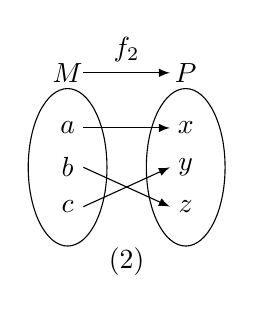
\begin{tikzpicture}[>=latex]
      \draw (0,0) ellipse (0.5 and 1);
      \draw (0,0.5) node {$a$} (0,0) node {$b$} (0,-0.5) node {$c$};
      \draw (1.5,0) ellipse (0.5 and 1);
      \draw (1.5,0.5) node {$x$} (1.5,0) node {$y$} (1.5,-0.5) node {$z$};
      \draw [->] (0.2,0.5) -- (1.3,0.5);
      \draw [->] (0.2,0) -- (1.3,-0.5);
      \draw [->] (0.2,-0.5) -- (1.3,0);
      \draw [->] (0.2,1.2) -- (1.3,1.2);
      \draw (0,1.2) node {$M$} (1.5,1.2) node{$P$};
      \draw (0.75,1.5) node {$f_2$} (0.75,-1.2) node {(2)};
  \end{tikzpicture}
  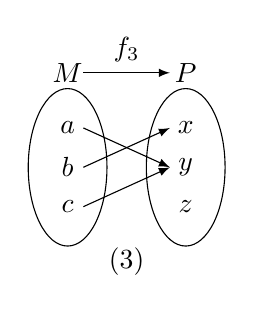
\begin{tikzpicture}[>=latex]
    \draw (0,0) ellipse (0.5 and 1);
    \draw (0,0.5) node {$a$} (0,0) node {$b$} (0,-0.5) node {$c$};
    \draw (1.5,0) ellipse (0.5 and 1);
    \draw (1.5,0.5) node {$x$} (1.5,0) node {$y$} (1.5,-0.5) node {$z$};
    \draw [->] (0.2,0.5) -- (1.3,0);
    \draw [->] (0.2,0) -- (1.3,0.5);
    \draw [->] (0.2,-0.5) -- (1.3,0);
    \draw [->] (0.2,1.2) -- (1.3,1.2);
    \draw (0,1.2) node {$M$} (1.5,1.2) node{$P$};
    \draw (0.75,1.5) node {$f_3$} (0.75,-1.2) node {(3)};
\end{tikzpicture}
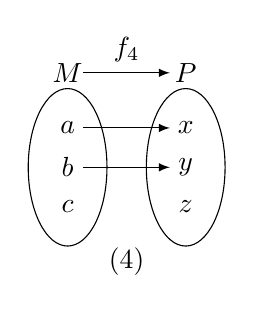
\begin{tikzpicture}[>=latex]
  \draw (0,0) ellipse (0.5 and 1);
  \draw (0,0.5) node {$a$} (0,0) node {$b$} (0,-0.5) node {$c$};
  \draw (1.5,0) ellipse (0.5 and 1);
  \draw (1.5,0.5) node {$x$} (1.5,0) node {$y$} (1.5,-0.5) node {$z$};
  \draw [->] (0.2,0.5) -- (1.3,0.5);
  \draw [->] (0.2,0) -- (1.3,0);
  \draw [->] (0.2,1.2) -- (1.3,1.2);
  \draw (0,1.2) node {$M$} (1.5,1.2) node{$P$};
  \draw (0.75,1.5) node {$f_4$} (0.75,-1.2) node {(4)};
\end{tikzpicture}
\end{center}
\twoch{只有$f_2,f_3$是从$M$到$P$的映射}{只有$f_2,f_4$是从$M$到$P$的映射}{只有$f_3,f_4$是从$M$到$P$的映射}{$f_1,f_2,f_3,f_4$都是从$M$到$P$的映射}
\item {\tiny (005286)}在给定的映射$f:(x,y)\mapsto (2x+y,xy)$($x,y\in \mathbf{R}$)下, 点$(\dfrac 16,-\dfrac 16)$的原像是\bracket{20}.
\fourch{$(\dfrac 16,-\dfrac 1{36})$}{$(\dfrac 13,-\dfrac 12)$或$(-\dfrac 14,\dfrac 23)$}{$(\dfrac 1{36},-\dfrac 16)$}{$(\dfrac 12,-\dfrac 13)$或$(-\dfrac 23,\dfrac 14)$}
\item {\tiny (005300)}在\textcircled{1} $y=x$与$y=\sqrt {x^2}$; \textcircled{2} $y=\sqrt {x^2}$与$y=(\sqrt x)^2$; \textcircled{3} $y=|x|$与$y=\dfrac{x^2}x$; \textcircled{4} $y=|x|$与$y=\sqrt {x^2}$; \textcircled{5} $y=x^0$与$y=1$这五组函数中, 表示同一函数的组数是\bracket{20}.
\fourch{$0$}{$1$}{$2$}{$3$}
\item {\tiny (005302)}已知镭经过$100$年后剩下原来质量的$95.76\%$, 若质量为$l$克的镭经过$x$年后的剩余质量为$y$克, 则$y$与$x$之间的解析式是\bracket{20}.
\fourch{$y=(\dfrac{0.9576}{100})^x$}{$y=(0.9576)^{100x}$}{$y=(0.9576)^{\frac x{100}}$}{$y=1-(1-0.9576)^{\frac x{100}}$}
\item {\tiny (005303)}函数$y=x+\dfrac{|x|}x$的图像是\bracket{20}.
\fourch{\begin{tikzpicture}[scale = 0.7,>=latex]
\draw [->] (-2,0) -- (2,0) node [below] {$x$};
\draw [->] (0,-2) -- (0,2) node [left] {$y$};
\draw (0,0) node [below right] {$O$};
\draw (-1,0) node [below] {$-1$} (0,1) node [right] {$1$};
\draw (-2,-1) -- (1,2);
\filldraw [white] (0,1) circle (0.05);
\draw (0,1) circle (0.05);
\end{tikzpicture}}{\begin{tikzpicture}[scale = 0.7,>=latex]
\draw [->] (-2,0) -- (2,0) node [below] {$x$};
\draw [->] (0,-2) -- (0,2) node [left] {$y$};
\draw (0,0) node [above left] {$O$};
\draw (1,0) node [below] {$1$} (0,-1) node [right] {$-1$};
\draw (-1,-2) -- (2,1);
\filldraw [white] (0,-1) circle (0.05);
\draw (0,-1) circle (0.05);
\end{tikzpicture}}{\begin{tikzpicture}[scale = 0.7,>=latex]
\draw [->] (-2,0) -- (2,0) node [below] {$x$};
\draw [->] (0,-2) -- (0,2) node [left] {$y$};
\draw (0,0) node [below right] {$O$};
\draw (1,0.1) -- (1,0) node [below] {$1$} (0,-1) node [right] {$-1$} (0,1) node [right] {$1$} (-1,0.1) -- (-1,0) node [below] {$-1$};
\draw (-1,-2) -- (0,-1) (0,1) -- (1,2);
\filldraw [white] (0,-1) circle (0.05);
\draw (0,-1) circle (0.05);
\filldraw [white] (0,1) circle (0.05);
\draw (0,1) circle (0.05);
\end{tikzpicture}}{\begin{tikzpicture}[scale = 0.7,>=latex]
\draw [->] (-2,0) -- (2,0) node [below] {$x$};
\draw [->] (0,-2) -- (0,2) node [left] {$y$};
\draw (0,0) node [below right] {$O$};
\draw (0,-1) node [right] {$-1$} (0,1) node [right] {$1$} (-1,0.1) -- (-1,0) node [below] {$-1$};
\draw (-2,1) -- (0,-1) (0,1) -- (1,2);
\filldraw [white] (0,-1) circle (0.05);
\draw (0,-1) circle (0.05);
\filldraw [white] (0,1) circle (0.05);
\draw (0,1) circle (0.05);
\end{tikzpicture}}
\item {\tiny (005377)}已知$n\in \mathbf{N}$, 在\textcircled{1} $\sqrt [4]{(-4)^{2n}}$; \textcircled{2} $\sqrt [4]{(-4)^{2n+1}}$; \textcircled{3} $\sqrt [5]{-x^2}$; \textcircled{4} $\sqrt [5]{-x^2}$这四个式子中, 有意义的\bracket{20}.
\fourch{是\textcircled{1}\textcircled{2}\textcircled{3}\textcircled{4} }{只有\textcircled{3}\textcircled{4}}{只有\textcircled{1}\textcircled{3}\textcircled{4}}{只有\textcircled{4}}
\item {\tiny (005386)}将$(a^{\frac 1n}+b^{\frac 1n})^{\frac 13}$表示成根式的形式是\bracket{20}.
\fourch{$\sqrt [3]{a^{\frac 1n}+b^{\frac 1n}}$}{$(\sqrt[n]a+\sqrt[n]b)^{\frac 13}$}{$\sqrt [3]{\sqrt[n]a+\sqrt[n]b}$}{$(\sqrt[n]a+\sqrt[n]b)^3$}
\item {\tiny (005448)}函数$f(x)=x^{\frac 23}$的图像是\bracket{20}.
\fourch{\begin{tikzpicture}[scale = 0.7, >=latex]
\draw [->] (-2,0) -- (2,0) node [below] {$x$};
\draw [->] (0,-2) -- (0,2) node [left] {$y$};
\draw (0,0) node [below left] {$O$};
\draw (1,0.2) -- (1,0) node [below] {$1$};
\draw (0.2,1) -- (0,1) node [left] {$1$};
\draw [domain = 0:4,samples = 400] plot ({\x^(1/2)},{\x^(1/3)});
\end{tikzpicture}}{\begin{tikzpicture}[scale = 0.7, >=latex]
\draw [->] (-2,0) -- (2,0) node [below] {$x$};
\draw [->] (0,-2) -- (0,2) node [left] {$y$};
\draw (0,0) node [below left] {$O$};
\draw (1,0.2) -- (1,0) node [below] {$1$};
\draw (0.2,1) -- (0,1) node [left] {$1$};
\draw (-1,0.2) -- (-1,0) node [below] {$-1$};
\draw [domain = 0:4,samples = 400] plot ({\x^(1/3)},{\x^(1/2)});
\draw [domain = 0:4,samples = 400] plot ({-\x^(1/3)},{\x^(1/2)});
\end{tikzpicture}}{\begin{tikzpicture}[scale = 0.7, >=latex]
\draw [->] (-2,0) -- (2,0) node [below] {$x$};
\draw [->] (0,-2) -- (0,2) node [left] {$y$};
\draw (0,0) node [below left] {$O$};
\draw (1,0.2) -- (1,0) node [below] {$1$};
\draw (0.2,1) -- (0,1) node [left] {$1$};
\draw (-1,0.2) -- (-1,0) node [below] {$-1$};
\draw [domain = 0:4,samples = 400] plot ({\x^(1/2)},{\x^(1/3)});
\draw [domain = 0:4,samples = 400] plot ({-\x^(1/2)},{\x^(1/3)});
\end{tikzpicture}}{\begin{tikzpicture}[scale = 0.7, >=latex]
\draw [->] (-2,0) -- (2,0) node [below] {$x$};
\draw [->] (0,-2) -- (0,2) node [left] {$y$};
\draw (0,0) node [below left] {$O$};
\draw (1,0.2) -- (1,0) node [below] {$1$};
\draw (0.2,1) -- (0,1) node [left] {$1$};
\draw (-1,0.2) -- (-1,0) node [below] {$-1$};
\draw (0.2,-1) -- (0,-1) node [left] {$-1$};
\draw [domain = 0:4,samples = 400] plot ({\x^(1/2)},{\x^(1/3)});
\draw [domain = 0:4,samples = 400] plot ({-\x^(1/2)},{-\x^(1/3)});
\end{tikzpicture}}
\item {\tiny (005449)}幂函数$y=x^m$和$y=x^n$在第一象限内的图像$C_1$和$C_2$图像所示, 则$m,n$之间的关系是\bracket{20}.
\begin{center}
    \begin{tikzpicture}[>=latex]
        \draw [->] (-1,0) -- (3,0) node [below] {$x$};
        \draw [->] (0,-1) -- (0,3) node [left] {$y$};
        \draw (0,0) node [below left] {$O$};
        \draw (1,0.2) -- (1,0) node [below] {$1$};
        \draw (0.2,1) -- (0,1) node [left] {$1$};
        \draw [domain = 0.5:2, samples = 400] plot (\x,{\x^(-5/4)});
        \draw [domain = 0.5:2, samples = 400] plot ({\x^(-5/4)},\x);
        \draw (0.5,{0.5^(-5/4)}) node [right] {$C_2$} ({0.5^(-5/4)},0.5) node [above] {$C_1$};
    \end{tikzpicture}
\end{center}
\fourch{$n<m<0$}{$m<n<0$}{$n>m>0$}{$m>n>0$}
\item {\tiny (005450)}图中, $C_1,C_2,C_3$为幂函数$y=x^a$在第一象限的图像, 则解析式中的指数$\alpha$依次可以取\bracket{20}.
\begin{center}
    \begin{tikzpicture}[>=latex]
        \draw [->] (-1,0) -- (3,0) node [below] {$x$};
        \draw [->] (0,-1) -- (0,3) node [left] {$y$};
        \draw (0,0) node [below left] {$O$};
        \draw (1,0.2) -- (1,0) node [below] {$1$};
        \draw (0.2,1) -- (0,1) node [left] {$1$};
        \draw [domain = {sqrt(3)/3}:3, samples = 400] plot (\x,{\x^(-2)});
        \draw [domain = 0:3, samples = 400] plot (\x,{\x^(3/4)});
        \draw [domain = 0:{3^(3/4)}, samples = 400] plot (\x,{\x^(4/3)});
        \draw (3,{1/9}) node [right] {$C_3$} (3,{3^(3/4)}) node [right] {$C_2$} ({3^(3/4)},3) node [above] {$C_1$};
    \end{tikzpicture}
\end{center}
\fourch{$\dfrac 43,-2,\dfrac 34$}{$-2,\dfrac 34,\dfrac 43$}{$-2,\dfrac 43,\dfrac 34$}{$\dfrac 34,\dfrac 43,-2$}
\item {\tiny (005459)}将下列函数图像的标号, 填在相应函数后面的横线上:\\
(1) $y=x^{\frac 23}$:\blank{50}; (2) $y=x^{-2}$:\blank{50}; (3) $y=x^{\frac 12}$:\blank{50};\\
(4) $y=x^{-1}$:\blank{50}; (5) $y=x^{\frac 13}$:\blank{50}; (6)$y=x^{\frac 32}$:\blank{50};\\ (7)$y=x^{\frac 43}$:\blank{50}; (8)$y=x^{-\frac 12}$:\blank{50}; (9)$y=x^{\frac 53}$:\blank{50}.
\begin{center}
    \begin{tikzpicture}[>=latex,scale = 0.6]
        \draw [->] (-2.5,0) -- (2.5,0) node [below] {$x$};
        \draw [->] (0,-2.5) -- (0,2.5) node [left] {$y$};
        \draw (0,0) node [below left] {$O$};
        \draw (0.2,1) -- (0,1) node [left] {$1$} (0.2,-1) -- (0,-1) node [left] {$-1$};
        \draw (1,0.2) -- (1,0) node [below] {$1$} (-1,0.2) -- (-1,0) node [below] {$1$};
        \draw (0,-2.5) node [below] {(A)};
        \draw [domain = 0:2.4, samples = 400] plot (\x,{\x^(1/2)});
    \end{tikzpicture}
    \begin{tikzpicture}[>=latex,scale = 0.6]
        \draw [->] (-2.5,0) -- (2.5,0) node [below] {$x$};
        \draw [->] (0,-2.5) -- (0,2.5) node [left] {$y$};
        \draw (0,0) node [below left] {$O$};
        \draw (0,-2.5) node [below] {(B)};
        \draw (0.2,1) -- (0,1) node [left] {$1$} (0.2,-1) -- (0,-1) node [left] {$-1$};
        \draw (1,0.2) -- (1,0) node [below] {$1$} (-1,0.2) -- (-1,0) node [below] {$1$};
        \draw [domain = 0:2.4, samples = 400] plot (\x,{\x^(1/3)});
        \draw [domain = 0:2.4, samples = 400] plot (-\x,{-\x^(1/3)});
    \end{tikzpicture}
    \begin{tikzpicture}[>=latex,scale = 0.6]
        \draw [->] (-2.5,0) -- (2.5,0) node [below] {$x$};
        \draw [->] (0,-2.5) -- (0,2.5) node [left] {$y$};
        \draw (0,0) node [below left] {$O$};
        \draw (0,-2.5) node [below] {(C)};
        \draw (0.2,1) -- (0,1) node [left] {$1$} (0.2,-1) -- (0,-1) node [left] {$-1$};
        \draw (1,0.2) -- (1,0) node [below] {$1$} (-1,0.2) -- (-1,0) node [below] {$1$};
        \draw [domain = {1/sqrt(2.4)}:2.4, samples = 400] plot (\x,{\x^(-2)});
        \draw [domain = {1/sqrt(2.4)}:2.4, samples = 400] plot (-\x,{\x^(-2)});
    \end{tikzpicture}\\
    \begin{tikzpicture}[>=latex,scale = 0.6]
        \draw [->] (-2.5,0) -- (2.5,0) node [below] {$x$};
        \draw [->] (0,-2.5) -- (0,2.5) node [left] {$y$};
        \draw (0,0) node [below left] {$O$};
        \draw (0,-2.5) node [below] {(D)};
        \draw (0.2,1) -- (0,1) node [left] {$1$} (0.2,-1) -- (0,-1) node [left] {$-1$};
        \draw (1,0.2) -- (1,0) node [below] {$1$} (-1,0.2) -- (-1,0) node [below] {$1$};
        \draw [domain = 0:{2.4^(3/4)}, samples = 400] plot (\x,{\x^(4/3)});
        \draw [domain = 0:{2.4^(3/4)}, samples = 400] plot (-\x,{\x^(4/3)});
    \end{tikzpicture}
    \begin{tikzpicture}[>=latex,scale = 0.6]
        \draw [->] (-2.5,0) -- (2.5,0) node [below] {$x$};
        \draw [->] (0,-2.5) -- (0,2.5) node [left] {$y$};
        \draw (0,0) node [below left] {$O$};
        \draw (0,-2.5) node [below] {(E)};
        \draw (0.2,1) -- (0,1) node [left] {$1$} (0.2,-1) -- (0,-1) node [left] {$-1$};
        \draw (1,0.2) -- (1,0) node [below] {$1$} (-1,0.2) -- (-1,0) node [below] {$1$};
        \draw [domain = 0:2.4, samples = 400] plot (\x,{\x^(2/3)});
        \draw [domain = 0:2.4, samples = 400] plot (-\x,{\x^(2/3)});
    \end{tikzpicture}
    \begin{tikzpicture}[>=latex,scale = 0.6]
        \draw [->] (-2.5,0) -- (2.5,0) node [below] {$x$};
        \draw [->] (0,-2.5) -- (0,2.5) node [left] {$y$};
        \draw (0,0) node [below left] {$O$};
        \draw (0,-2.5) node [below] {(F)};
        \draw (0.2,1) -- (0,1) node [left] {$1$} (0.2,-1) -- (0,-1) node [left] {$-1$};
        \draw (1,0.2) -- (1,0) node [below] {$1$} (-1,0.2) -- (-1,0) node [below] {$1$};
        \draw [domain = 0:{2.4^(3/5)}, samples = 400] plot (\x,{\x^(5/3)});
        \draw [domain = 0:{2.4^(3/5)}, samples = 400] plot (-\x,{-\x^(5/3)});
    \end{tikzpicture}\\
    \begin{tikzpicture}[>=latex,scale = 0.6]
        \draw [->] (-2.5,0) -- (2.5,0) node [below] {$x$};
        \draw [->] (0,-2.5) -- (0,2.5) node [left] {$y$};
        \draw (0,0) node [below left] {$O$};
        \draw (0,-2.5) node [below] {(G)};
        \draw (0.2,1) -- (0,1) node [left] {$1$} (0.2,-1) -- (0,-1) node [left] {$-1$};
        \draw (1,0.2) -- (1,0) node [below] {$1$} (-1,0.2) -- (-1,0) node [below] {$1$};
        \draw [domain = {1/2.4}:2.4] plot (\x,{1/\x});
        \draw [domain = {1/2.4}:2.4] plot (-\x,{-1/\x});
    \end{tikzpicture}
    \begin{tikzpicture}[>=latex,scale = 0.6]
        \draw [->] (-2.5,0) -- (2.5,0) node [below] {$x$};
        \draw [->] (0,-2.5) -- (0,2.5) node [left] {$y$};
        \draw (0,0) node [below left] {$O$};
        \draw (0,-2.5) node [below] {(H)};
        \draw (0.2,1) -- (0,1) node [left] {$1$} (0.2,-1) -- (0,-1) node [left] {$-1$};
        \draw (1,0.2) -- (1,0) node [below] {$1$} (-1,0.2) -- (-1,0) node [below] {$1$};
        \draw [domain = {1/2.4^2}:2.4] plot (\x,{1/\x^(1/2)});
    \end{tikzpicture}
    \begin{tikzpicture}[>=latex,scale = 0.6]
        \draw [->] (-2.5,0) -- (2.5,0) node [below] {$x$};
        \draw [->] (0,-2.5) -- (0,2.5) node [left] {$y$};
        \draw (0,0) node [below left] {$O$};
        \draw (0,-2.5) node [below] {(I)};
        \draw (0.2,1) -- (0,1) node [left] {$1$} (0.2,-1) -- (0,-1) node [left] {$-1$};
        \draw (1,0.2) -- (1,0) node [below] {$1$} (-1,0.2) -- (-1,0) node [below] {$1$};
        \draw [domain = 0:{2.4^(2/3)}] plot (\x,{\x^(3/2)});
    \end{tikzpicture}
\end{center}
\item {\tiny (005462)}函数$f(x)=x^{k^2-2k-3}$($k\in \mathbf{Z}$)的图像如图所示, 则$k=$\blank{50}.
\begin{center}
    \begin{tikzpicture}[>=latex]
        \draw [->] (-2.5,0) -- (2.5,0) node [below] {$x$};
        \draw [->] (0,-0.5) -- (0,2.5) node [left] {$y$};
        \draw (0,0) node [below left] {$O$};
        \draw (0,-0.5) node [below] {(C)};
        \draw (0.2,1) -- (0,1) node [left] {$1$};
        \draw (1,0.2) -- (1,0) node [below] {$1$} (-1,0.2) -- (-1,0) node [below] {$1$};
        \draw [domain = {1/2.4^(1/4)}:2.4, samples = 400] plot (\x,{\x^(-4)});
        \draw [domain = {1/2.4^(1/4)}:2.4, samples = 400] plot (-\x,{\x^(-4)});
    \end{tikzpicture}
\end{center}
\item {\tiny (005527)}若函数$y=g(x)$的图像与函数$f(x)=(x-1)^2$($x\le 1$)的图像关于直线$y=x$对称.则$g(x)$的表达式是\bracket{20}.
\twoch{$g(x)=1-\sqrt x$($x\ge 0$)}{$g(x)=1+\sqrt x$($x\ge 0$)}{$g(x)=\sqrt {1-x}$($x\le 1$)}{$g(x)=\sqrt {1+x}$($x\ge -1$)}
\item {\tiny (005561)}填写下表:
\begin{center}
    \begin{tabular}{|c|c|c|c|c|}
        \hline
        $x$	 & $f(x)=x^2$ & $f(x)-f(x-1)$ & $g(x)=2^x$ & $g(x)-g(x-1)$ \\ \hline
        $0$ & & & & \\ \hline
        $1$ & & & & \\ \hline
        $2$ & & & & \\ \hline
        $3$ & & & & \\ \hline
        $4$ & & & & \\ \hline
        $5$ & & & & \\ \hline
        $6$ & & & & \\ \hline
        $7$ & & & & \\ \hline
        $8$ & & & & \\ \hline
        $9$ & & & & \\ \hline
        $10$ & & & & \\ \hline
    \end{tabular}
\end{center}
(1) 比较$f(x)=x^2$与$g(x)=2^x$的函数值的大小;\\
(2) 比较$f(x)=x^2$与$g(x)=2^x$的函数值递增的快慢.
\item {\tiny (005562)}已知函数$f(x)=2x+1$, $g(x)=1.5^x$, $h(x)=x^{1.5}$, 试用数值计算比较三个函数在$[0,+\infty)$上的函数值的大小、图像递增的快慢. 并说明在函数图像上的表现.
解  列表并计算得:
\begin{center}
    \begin{longtable}{|c|c|c|c|c|c|c|}
        \hline
        $x$	 & $f(x)=2x+1$ & $f(x)-f(x-1)$ & $g(x)=1.5^x$ & $g(x)-g(x-1)$ & $h(x)=x^{1.5}$ & $h(x)-h(x-1)$ \\ \hline
        \endhead
        $0$ & $1$ & & $1$ & & $0$ &  \\ \hline
        $1$ & $3$ & $2$ & $1.5$ & $0.5$ & $1$ & $1$\\ \hline
        $2$ & $5$ & $2$ & $2.25$ & $0.75$ & $2.82842712$ & $1.82842712$\\ \hline
        $3$ & $7$ & $2$ & $3.375$ & $1.125$ & $5.19615242$ & $2.3677253$\\ \hline
        $4$ & $9$ & $2$ & $5.0625$ & $1.6875$ & $8$ & $2.80384758$\\ \hline
        $5$ & $11$ & $2$ & $7.59375$ & $2.53125$ & $11.1803399$ & $3.18033989$\\ \hline
        $6$ & $13$ & $2$ & $11.390625$ & $3.796875$ & $14.6969385$ & $3.51659857$\\ \hline
        $7$ & $15$ & $2$ & $17.085938$ & $5.6953125$ & $18.5202592$ & $3.82332072$\\ \hline
        $8$ & $17$ & $2$ & $25.628906$ & $8.5429688$ & $22.627417$ & $4.10715782$\\ \hline
        $9$ & $19$ & $2$ & $38.443359$ & $12.814453$ & $27$ & $4.372583$\\ \hline
        $10$ & $21$ & $2$ & $57.665039$ & $19.22168$ & $31.6227766$ & $4.6227766$\\ \hline
        $11$ & $23$ & $2$ & $86.497559$ & $28.83252$ & $36.4828727$ & $4.86009609$\\ \hline
        $12$ & $25$ & $2$ & $129.74634$ & $43.248779$ & $41.5692194$ & $5.08634669$\\ \hline
        $13$ & $27$ & $2$ & $194.61951$ & $64.873169$ & $46.8721666$ & $5.3029472$\\ \hline
        $14$ & $29$ & $2$ & $291.92926$ & $97.309753$ & $52.3832034$ & $5.51103683$\\ \hline
        $15$ & $31$ & $2$ & $437.89389$ & $145.96463$ & $58.0947502$ & $5.71154678$\\ \hline
        $16$ & $33$ & $2$ & $656.84084$ & $218.94695$ & $64$ & $5.90524981$\\ \hline
        $17$ & $35$ & $2$ & $985.26125$ & $328.42042$ & $70.0927956$ & $6.09279564$\\ \hline
        $18$ & $37$ & $2$ & $1477.8919$ & $492.63063$ & $76.3675324$ & $6.27473673$\\ \hline
        $19$ & $39$ & $2$ & $2216.8378$ & $738.94594$ & $82.8190799$ & $6.45154756$\\ \hline
        $20$ & $41$ & $2$ & $3325.2567$ & $1108.4189$ & $89.4427191$ & $6.62363917$\\ \hline
        $21$ & $43$ & $2$ & $4987.8851$ & $1662.6284$ & $96.2340896$ & $6.79137049$\\ \hline
        $22$ & $45$ & $2$ & $7481.8276$ & $2493.9425$ & $103.189147$ & $6.95505712$\\ \hline
        $23$ & $47$ & $2$ & $11222.741$ & $3740.9138$ & $110.304125$ & $7.11497832$\\ \hline
        $24$ & $49$ & $2$ & $16834.112$ & $5611.3707$ & $117.575508$ & $7.27138262$\\ \hline
        $25$ & $51$ & $2$ & $25251.168$ & $8417.0561$ & $125$ & $7.42449235$\\ \hline
        $26$ & $53$ & $2$ & $37876.752$ & $12625.584$ & $132.574507$ & $7.57450735$\\ \hline
        $27$ & $55$ & $2$ & $56815.129$ & $18938.376$ & $140.296115$ & $7.72160806$\\ \hline
        $28$ & $57$ & $2$ & $85222.693$ & $28407.564$ & $148.162073$ & $7.86595801$\\ \hline
        $29$ & $59$ & $2$ & $127834.04$ & $42611.346$ & $156.169779$ & $8.00770599$\\ \hline
        $30$ & $61$ & $2$ & $191751.06$ & $63917.02$ & $164.316767$ & $8.14698784$\\ \hline
        $\cdots$ & $\cdots$ & $\cdots$ & $\cdots$ & $\cdots$ & $\cdots$ & $\cdots$ \\ \hline
    \end{longtable}
\end{center}
得点$A,B,C,D$的横坐标分别约为$1.5,4.8, 6.5, 7.4$, 记作$x_A,x_B,x_C,x_D$.\\
(1) 三个函数的函数值的大小情况如下:\\
\textcircled{1} 当$0<x<x_A$时, $f(x)>g(x)>h(x)$;
\textcircled{2} 当$x_A<x<x_B$时, $f(x)>h(x)>g(x)$;
\textcircled{3} 由$x_B<x<x_C$时, $h(x)>f(x)>g(x)$;
\textcircled{4} 当$x_C<x<x_D$时, $h(x)>g(x)>f(x)$;
\textcircled{5} 当$x_D<x$时, $g(x)>h(x)>f(x)$;
\textcircled{6} 当$x=x_A$时, $f(x)>g(x)=h(x)$;
\textcircled{7} 当$x=x_B$时, $f(x)=h(x)>g(x)$;
\textcircled{8} 当$x=x_C$时, $f(x)=g(x)<h(x)$;
\textcircled{9} 当$x=x_D$时, $f(x)<g(x)=g(x)$.\\
(2) 它们在同一个平面直角坐标系下的图像如图14所示.
\begin{center}
    \begin{tikzpicture}[>=latex]
        \draw [->] (-0.1,0) -- (5,0) node [below] {$x$};
        \draw [->] (0,-0.1) -- (0,5.75) node [left] {$y$};
        \draw (0,0) node [below left] {$O$};
        \draw [domain = 0:9,samples = 100, name path = firstorder] plot ({\x/2},{(2*\x+1)/4});
        \draw (4.5,{19/4}) node [right] {$y=f(x)$};
        \draw [domain = 0:7.8, samples = 100, name path = exponential] plot ({\x/2},{1.5^(\x)/4}); 
        \draw (3.9,{1.5^7.8/4}) node [above right] {$y=g(x)$};
        \draw [domain = 0:8, samples = 100, name path = power] plot ({\x/2},{\x^(3/2)/4});
        \draw (4,{8^(3/2)/4}) node [below right] {$y=h(x)$};
        \path [name intersections = {of = firstorder and exponential, by = {T,C}}];
        \path [name intersections = {of = firstorder and power, by = B}];
        \path [name intersections = {of = exponential and power, by = {A,D}}];
        \filldraw (A) circle (0.05) node [below right] {$A$};
        \filldraw (B) circle (0.05) node [below right] {$B$};
        \filldraw (C) circle (0.05) node [below right] {$C$};
        \filldraw (D) circle (0.05) node [below right] {$D$};
        \foreach \i in {1,2,...,9}{\draw (\i/2,0.1) -- (\i/2,0) node [below] {$\i$};};
        \foreach \i in {1,3,...,21}{\draw (0.1,\i/4) -- (0,\i/4) node [left] {$\i$};};
    \end{tikzpicture}
\end{center}
由表格及图像可看出, 三个函数的函数值变化及相应增量规律为: 随着$x$的增大, 直线型均匀上升, 增量恒定; 指数型急剧上升, 在区间$[0,+\infty)$上递增增量快速增大; 幂函数型虽上升较快, 但随着$x$的不断增大上升趋势远不如指数型, 几乎微不足道, 其增量缓慢递增.
\item {\tiny (005567)}若$f(x)=\dfrac{\mathrm{e}^x-\mathrm{e}^{-x}}2$, $g(x)=\dfrac{\mathrm{e}^x+\mathrm{e}^{-x}}2$.则下列关系式中不正确的是\bracket{20}.
\twoch{$[g(x)]^2-[f(x)]^2=1$}{$f(2x)=2f(x)\cdot g(x)$}{$g(2x)=[f(x)]^2+[g(x)]^2$}{$f(-x)g(x)=f(x)g(-x)$}
\item {\tiny (005568)}若$a>b$且$ab\ne 0$.则在\textcircled{1} $a^2>b^2$, \textcircled{2} $2^a>2^b$, \textcircled{3} $\dfrac 1a<\dfrac 1b$, \textcircled{4} $a^{\frac 13}>b^{\frac 13}$, \textcircled{5} $(\dfrac 13)^a<(\dfrac 13)^b$这五个关系式中, 恒成立的有\bracket{20}.
\fourch{$1$个}{$2$个}{$3$个}{$4$个}
\item {\tiny (005569)}在同一平面直角坐标系中, 函数$f(x)=ax$与$g(x)=a^x$的图像可能是\bracket{20}.
\fourch{\begin{tikzpicture}[scale = 0.15, >=latex]
    \draw [->] (-8,0) -- (8,0) node [below] {$x$};
    \draw [->] (0,-4) -- (0,12) node [left] {$y$};
    \draw (0,0) node [below left] {$O$};
    \draw [domain = -6:2, samples = 100] plot (\x,{-1.5*\x});
    \draw [domain = -6:6, samples = 100] plot (\x,{1.5^\x});
\end{tikzpicture}}{\begin{tikzpicture}[scale = 0.15, >=latex]
    \draw [->] (-8,0) -- (8,0) node [below] {$x$};
    \draw [->] (0,-4) -- (0,12) node [left] {$y$};
    \draw (0,0) node [below left] {$O$};
    \draw [domain = -2:6, samples = 100] plot (\x,{1.5*\x});
    \draw [domain = -6:6, samples = 100] plot (-\x,{1.5^\x});
\end{tikzpicture}}{\begin{tikzpicture}[scale = 0.15, >=latex]
    \draw [->] (-8,0) -- (8,0) node [below] {$x$};
    \draw [->] (0,-4) -- (0,12) node [left] {$y$};
    \draw (0,0) node [below left] {$O$};
    \draw [domain = -2:6, samples = 100] plot (\x,{1.5*\x});
    \draw [domain = -6:6, samples = 100] plot (\x,{1.5^\x});
\end{tikzpicture}}{\begin{tikzpicture}[scale = 0.15, >=latex]
    \draw [->] (-8,0) -- (8,0) node [below] {$x$};
    \draw [->] (0,-4) -- (0,12) node [left] {$y$};
    \draw (0,0) node [below left] {$O$};
    \draw [domain = -2:6, samples = 100] plot (-\x,{1.5*\x});
    \draw [domain = -6:6, samples = 100] plot (-\x,{1.5^\x});
\end{tikzpicture}}
\item {\tiny (005570)}下列各式中, 正确的是\bracket{20}.
\fourch{$(\dfrac 12)^{\frac 23}<(\dfrac 15)^{\frac 23}<(\dfrac 12)^{\frac 13}$}{$(\dfrac 12)^{\frac 13}<(\dfrac 12)^{\frac 23}<(\dfrac 15)^{\frac 23}$}{$(\dfrac 15)^{\frac 23}<(\dfrac 12)^{\frac 13}<(\dfrac 12)^{\frac 23}$}{$(\dfrac 15)^{\frac 23}<(\dfrac 12)^{\frac 23}<(\dfrac 12)^{\frac 13}$}
\item {\tiny (005575)}用不等号``$>$''或``$<$''填空:
(1) $1.2^{0.3}$\blank{50}$1$;\\
(2) $0.3^{5.1}$\blank{50}$1$;\\
(3) $(\dfrac 23)^{-\frac 13}$\blank{50}$(\dfrac 32)^{-\frac 13}$;\\
(4) $9^{\frac 13}$\blank{50}$3^{\frac 43}$;\\
(5) $2^{\frac 23}$\blank{50}$3.6^{-\frac 34}$;\\
(6) $0.8^{-2}$\blank{50}$(\dfrac 53)^{-\frac 12}$.
\item {\tiny (005576)}将下列各数从小到大排列:
(1) $0.9^{\frac 34}$, $1.2^{\frac 34}$, 1:\blank{50};\\
(2) $2.5^{\frac 23}$, $(-1.4)^{\frac 23}$, $(-3)^{\frac 13}$:\blank{50};\\
(3) $4.1^{\frac 23}$, $3.8^{-\frac 23}$, $(-1.9)^{\frac 35}$:\blank{50}.
\item {\tiny (005577)}根据条件确定实数$x$的取值范围:\\
(1) $2^x>0.5$:\blank{50};\\
(2) $2^x<1$:\blank{50};\\
(3) $0.2^{2x-1}>\dfrac 1{25}$:\blank{50};\\
(4) $8<(\dfrac 12)^{2x+1}$:\blank{50};\\
(5) $(a^2+a+2)^x>(a^2+a+2)^{1-x}$:\blank{50};\\
(6) $(\dfrac 12)^{x^2+x-2}<1$:\blank{50}.
\item {\tiny (005606)}某地区不同身高的未成年男性的体重平均值如下表(身高: $\text{cm}$; 体重: $\text{kg}$):
\begin{center}
    \begin{tabular}{|c|c|c|c|c|c|c|}
        \hline
        身高 & $60$ & $70$ & $80$ & $90$ & $100$ & $110$\\ \hline
        体重 & $6.13$ & $7.90$ & $9.99$ & $12.15$ & $15.02$ & $17.05$\\ \hline
        身高 & $120$ & $130$ & $140$ & $150$ & $160$ & $170$\\ \hline
        体重 & $20.92$ & $26.86$ & $31.11$ & $38.85$ & $47.25$ & $55.05$\\ \hline
    \end{tabular}
\end{center}
为了揭示未成年男性的身高与体重的规律, 甲选择了模型$y=ax^2+bx+c$($a>0$), 乙选择了模型$y=ba^x$($a>1$), 其中$y$表示体重, $x$表示身高.你认为谁选择的模型较好?
\item {\tiny (005607)}用计算器计算并填写下表:
\begin{center}
    \begin{tabular}{|c|c|c|c|c|}
        \hline
        $x$	& $f(x)=x^{\frac 12}$ & $g(x)=x^{0.6}$ & $h(x)=2.1^x$ & $s(x)=2.2^x$ \\ \hline
        $0$ & & & & \\ \hline
        $1$ & & & & \\ \hline
        $2$ & & & & \\ \hline
        $3$ & & & & \\ \hline
        $4$ & & & & \\ \hline
        $5$ & & & & \\ \hline
        $6$ & & & & \\ \hline
        $7$ & & & & \\ \hline
        $8$ & & & & \\ \hline
        $9$ & & & & \\ \hline
        $10$ & & & & \\ \hline
    \end{tabular}
\end{center}
从表中变化的现象可以归纳出哪些函数递增的规律?\\
(1) 幂函数$f(x)$与$g(x)$之间比较得出的规律;
(2) 指数函数$h(x)$与$s(x)$之间比较得出的规律;
(3) 幂函数$f(x)=x^{\frac 12}$与指数函数$h(x)$之间比较得出的规律
\item {\tiny (005617)}给出下列四个式子(已知$a>0$, $a\ne 1$, $x>y>0$): \textcircled{1} $\log_ax\cdot \log_ay=\log_a(x+y)$; \textcircled{2} $\log_ax+\log_ay=\log_a(x+y)$; \textcircled{3} $\log_a\dfrac xy=\log_a(x-y)$; \textcircled{4} $\log_a(x-y)=\dfrac{\log_ax}{\log_ay}$.其中正确的有\bracket{20}.
\fourch{$0$个}{$1$个}{$2$个}{$3$个}
\item {\tiny (005658)}若$x\ne 1$, 则与$\dfrac 1{\log_3x}+\dfrac 1{\log_4x}+\dfrac 1{\log_5x}$相等的式子是\bracket{20}.
\fourch{$\dfrac 1{\log_{60}x}$}{$\dfrac 1{\log_3x\cdot \log_4x\cdot \log_5x}$}{$\dfrac 1{\log_x60}$}{$\dfrac{12}{\log_3 x+\log_4 x+\log_5 x}$}
\item {\tiny (005690)}图中图像所对应的函数可能是\bracket{20}.
\begin{center}
    \begin{tikzpicture}[>=latex]
        \draw [->] (-1,0) -- (3,0) node [below] {$x$};
        \draw [->] (0,-2) -- (0,2) node [left] {$y$};
        \draw (0,0) node [below left] {$O$};
        \draw [domain = -1.4:1.8] plot ({0.5^\x},\x);
        \draw (1,0) node [below] {$1$}; 
    \end{tikzpicture}
\end{center}
\fourch{$y=2^x$}{$y=2^x$的反函数}{$y=2^{-x}$}{$y=2^{-x}$的反函数}
\item {\tiny (005691)}设$f(x)$是定义在$(-\infty ,+\infty)$上的偶函数, 且它在$[0,+\infty)$上是增函数, 记$a=f(-\log_{\sqrt 2}\sqrt 3)$, $b=f(-\log_{\sqrt 3}\sqrt 2)$, $c=f(-2)$, 则$a,b,c$的大小关系是\bracket{20}.
\fourch{$a>b>c$}{$b>c>a$}{$c>a>b$}{$c>b>a$}
\item {\tiny (005692)}下列函数图像中, 不正确的是\bracket{20}.
\begin{center}
    \begin{tikzpicture}[>=latex, scale = 0.5]
        \draw [->] (-3,0) -- (3,0) node [below] {$x$};
        \draw [->] (0,-1.5) -- (0,3) node [left] {$y$};
        \draw (0,0) node [below left] {$O$};
        \draw (1,0) node [below] {$1$};
        \draw [domain = -1.4:2.5] plot ({sqrt((1/3)^\x)},\x);
        \draw [domain = -1.4:2.5] plot ({-sqrt((1/3)^\x)},\x);
        \draw (0,-1.5) node [below] {(A)};
    \end{tikzpicture}
    \begin{tikzpicture}[>=latex, scale = 0.5]
        \draw [->] (-3,0) -- (3,0) node [below] {$x$};
        \draw [->] (0,-1.5) -- (0,3) node [left] {$y$};
        \draw (0,0) node [below left] {$O$};
        \draw (1,0) node [below] {$1$};
        \draw [domain = -0.9:2.5] plot ({-(1/3)^\x},\x);
        \draw (0,-1.5) node [below] {(B)};
    \end{tikzpicture}
    \begin{tikzpicture}[>=latex, scale = 0.5]
        \draw [->] (-3,0) -- (3,0) node [below] {$x$};
        \draw [->] (0,-1.5) -- (0,3) node [left] {$y$};
        \draw (0,0) node [below left] {$O$};
        \draw (1,0) node [below] {$1$};
        \draw [domain = -0.9:2.5] plot ({(1/3)^\x},{abs(\x)});
        \draw (0,-1.5) node [below] {(C)};
    \end{tikzpicture}
    \begin{tikzpicture}[>=latex, scale = 0.5]
        \draw [->] (-3,0) -- (3,0) node [below] {$x$};
        \draw [->] (0,-1.5) -- (0,3) node [left] {$y$};
        \draw (0,0) node [below left] {$O$};
        \draw (1,0) node [below] {$1$};
        \draw [domain = 0.1:2.5] plot (\x,{\x^(-1/3)});
        \draw (0,-1.5) node [below] {(D)};
    \end{tikzpicture}
\end{center}
\fourch{$y=\log_{\frac 13}x^2$}{$y=\log_{\frac 13}(-x)$}{$y=|\log_3x|$}{$y=|x^{-\frac 13}|$}
\item {\tiny (005693)}在同一平面直角坐标系中画出函数$y=x+a$与$y=\log_ax$的图像, 可能是\bracket{20}.
\fourch{\begin{tikzpicture}[scale = 0.5, >=latex]
    \draw [->] (-2,0) -- (3,0) node [below] {$x$};
    \draw [->] (0,-2) -- (0,3) node [left] {$y$};
    \draw (0,0) node [below left] {$O$};
    \draw (1,0) node [below] {$1$};
    \draw (0.1,1) -- (0,1) node [left] {$1$};
    \draw [domain = -1.8:1.2] plot (\x,{\x+1.5});
    \draw [domain = -2.5:2] plot ({1.5^\x},{-\x}); 
\end{tikzpicture}}
{\begin{tikzpicture}[scale = 0.5, >=latex]
    \draw [->] (-2,0) -- (3,0) node [below] {$x$};
    \draw [->] (0,-2) -- (0,3) node [left] {$y$};
    \draw (0,0) node [below left] {$O$};
    \draw (1,0) node [below] {$1$};
    \draw (0.1,1) -- (0,1) node [left] {$1$};
    \draw [domain = -1.8:2.2] plot (\x,{\x+0.7}); 
    \draw [domain = -1.9:2.5] plot ({1.5^\x},{\x}); 
\end{tikzpicture}}
{\begin{tikzpicture}[scale = 0.5, >=latex]
    \draw [->] (-2,0) -- (3,0) node [below] {$x$};
    \draw [->] (0,-2) -- (0,3) node [left] {$y$};
    \draw (0,0) node [below left] {$O$};
    \draw (1,0) node [below] {$1$};
    \draw (0.1,1) -- (0,1) node [left] {$1$};
    \draw [domain = -1.8:2.2] plot (\x,{\x+0.7}); 
    \draw [domain = -1.9:2.5] plot ({0.7^\x},{\x}); 
\end{tikzpicture}}
{\begin{tikzpicture}[scale = 0.5, >=latex]
    \draw [->] (-2,0) -- (3,0) node [below] {$x$};
    \draw [->] (0,-2) -- (0,3) node [left] {$y$};
    \draw (0,0) node [below left] {$O$};
    \draw (1,0) node [below] {$1$};
    \draw (0.1,1) -- (0,1) node [left] {$1$};
    \draw [domain = -1.8:2.8] plot (\x,{\x-0.2}); 
    \draw [domain = -1.9:2.5] plot ({1.4^\x},{\x}); 
\end{tikzpicture}}
\item {\tiny (005694)}函数$y=f(x)$的图像如图所示, 则$y=\log_{0.7}f(x)$的示意图是\bracket{20}.
\begin{center}
    \begin{tikzpicture}[>=latex]
        \draw [->] (-0.5,0) -- (3,0) node [below] {$x$};
        \draw [->] (0,-0.5) -- (0,3) node [left] {$y$};
        \draw (0,0) node [below left] {$O$};
        \draw (1,0.1) -- (1,0) node [below] {$1$} (2,0.1) -- (2,0) node [below] {$2$} (0.1,1) -- (0,1) node [left] {$1$};
        \draw [dashed] (2,0) -- (2,3);
        \draw [dashed] (1,0) -- (1,1) -- (0,1);
        \draw [domain = 0.3:1.7] plot (\x,{3*(\x-1)^2+1});
    \end{tikzpicture}
\end{center}
\fourch{\begin{tikzpicture}[>=latex,scale = 0.6]
    \draw [->] (-0.5,0) -- (3,0) node [below] {$x$};
    \draw [->] (0,-3) -- (0,3) node [left] {$y$};
    \draw (0,0) node [below left] {$O$};
    \draw (1,0.1) -- (1,0) node [below] {$1$} (2,0.1) -- (2,0) node [below right] {$2$};
    \draw [dashed] (2,-3) -- (2,3);
    \draw [domain = 0.3:1] plot (\x,{ln(3*(\x-1)^2+1)/ln(0.7)});
    \draw [domain = 1:1.7] plot (\x,{-ln(3*(\x-1)^2+1)/ln(0.7)});
\end{tikzpicture}}{\begin{tikzpicture}[>=latex,scale = 0.6]
    \draw [->] (-0.5,0) -- (3,0) node [below] {$x$};
    \draw [->] (0,-3) -- (0,3) node [left] {$y$};
    \draw (0,0) node [below left] {$O$};
    \draw (1,0.1) -- (1,0) node [below] {$1$} (2,0.1) -- (2,0) node [below right] {$2$};
    \draw [dashed] (2,-3) -- (2,3);
    \draw [domain = 0.3:1] plot (\x,{-ln(3*(\x-1)^2+1)/ln(0.7)});
    \draw [domain = 1:1.7] plot (\x,{ln(3*(\x-1)^2+1)/ln(0.7)});
\end{tikzpicture}}{\begin{tikzpicture}[>=latex,scale = 0.6]
    \draw [->] (-0.5,0) -- (3,0) node [below] {$x$};
    \draw [->] (0,-3) -- (0,3) node [left] {$y$};
    \draw (0,0) node [below left] {$O$};
    \draw (1,0.1) -- (1,0) node [below] {$1$} (2,0.1) -- (2,0) node [below right] {$2$};
    \draw [dashed] (2,-3) -- (2,3);
    \draw [domain = 0.3:1.7] plot (\x,{ln(3*(\x-1)^2+1)/ln(0.7)});
\end{tikzpicture}}{\begin{tikzpicture}[>=latex,scale = 0.6]
    \draw [->] (-0.5,0) -- (3,0) node [below] {$x$};
    \draw [->] (0,-3) -- (0,3) node [left] {$y$};
    \draw (0,0) node [below left] {$O$};
    \draw (1,0.1) -- (1,0) node [below] {$1$} (2,0.1) -- (2,0) node [below right] {$2$};
    \draw [dashed] (2,-3) -- (2,3);
    \draw [domain = 0.3:1.7] plot (\x,{-ln(3*(\x-1)^2+1)/ln(0.7)});
\end{tikzpicture}}
\item {\tiny (005695)}由关系式$\log_xy=3$所确定的函数$y=f(x)$的图像是\bracket{20}.
\fourch{\begin{tikzpicture}[>=latex,scale = 0.7]
    \draw [->] (-2.3,0) -- (2.3,0) node [below] {$x$};
    \draw [->] (0,-2.3) -- (0,2.3) node [left] {$y$};
    \draw (0,0) node [below left] {$O$};
    \draw (1,0.1) -- (1,0) node [below] {$1$} (-1,0.1) -- (-1,0) node [below] {$-1$} (0.1,1) -- (0,1) node [left] {$1$} (0.1,-1) -- (0,-1) node [left] {$-1$};
    \draw [domain = 0:2] plot ({\x^(1/3)},\x);
    \draw [domain = 0:2] plot ({-\x^(1/3)},{-\x});
\end{tikzpicture}}{\begin{tikzpicture}[>=latex,scale = 0.7]
    \draw [->] (-2.3,0) -- (2.3,0) node [below] {$x$};
    \draw [->] (0,-2.3) -- (0,2.3) node [left] {$y$};
    \draw (0,0) node [below left] {$O$};
    \draw (1,0.1) -- (1,0) node [below] {$1$} (-1,0.1) -- (-1,0) node [below] {$-1$} (0.1,1) -- (0,1) node [left] {$1$} (0.1,-1) -- (0,-1) node [left] {$-1$};
    \draw [domain = 0:2] plot ({\x^(1/3)},\x);
    \filldraw [white] (0,0) circle (0.05) (1,1) circle (0.05);
    \draw (0,0) circle (0.05) (1,1) circle (0.05);
\end{tikzpicture}}{\begin{tikzpicture}[>=latex,scale = 0.7]
    \draw [->] (-2.3,0) -- (2.3,0) node [below] {$x$};
    \draw [->] (0,-2.3) -- (0,2.3) node [left] {$y$};
    \draw (0,0) node [below left] {$O$};
    \draw (1,0.1) -- (1,0) node [below] {$1$} (-1,0.1) -- (-1,0) node [below] {$-1$} (0.1,1) -- (0,1) node [left] {$1$} (0.1,-1) -- (0,-1) node [left] {$-1$};
    \draw [domain = 0:2] plot ({\x^(1/3)},\x);
\end{tikzpicture}}{\begin{tikzpicture}[>=latex,scale = 0.7]
    \draw [->] (-2.3,0) -- (2.3,0) node [below] {$x$};
    \draw [->] (0,-2.3) -- (0,2.3) node [left] {$y$};
    \draw (0,0) node [below left] {$O$};
    \draw (1,0.1) -- (1,0) node [below] {$1$} (-1,0.1) -- (-1,0) node [below] {$-1$} (0.1,1) -- (0,1) node [left] {$1$} (0.1,-1) -- (0,-1) node [left] {$-1$};
    \draw [domain = 0:2] plot ({\x^(1/3)},\x);
    \draw [domain = 0:2] plot ({-\x^(1/3)},\x);
\end{tikzpicture}}
\item {\tiny (005783)}关于$x$的方程$\log_ax^2=\log_a(\sqrt {a+1}-\sqrt a)-\log_a(\sqrt {a+1}+\sqrt a)$($a>0$且$a\ne 1$)的解为\bracket{20}.
\fourch{$\sqrt {a+1}+\sqrt a$}{$\sqrt {a+1}-\sqrt a$}{$\pm (\sqrt {a+1}+\sqrt a)$}{$\pm (\sqrt {a+1}-\sqrt a)$}
\item {\tiny (005850)}已知函数$f(x)=\log_3(x^2-4mx+4m^2+m+\dfrac 1{m-1})$, 集合$M=\{m|m>1,m\in \mathbf{R}\}$.\\
(1) 求证: 当$m\in M$时, $f(x)$的定义域为$x\in \mathbf{R}$; 反之, 若$f(x)$对一切实数$x$都有意义, 则$m\in M$;\\
(2) 当$m\in M$时, 求$f(x)$的最小值;\\
(3) 求证: 对每一个$m\in M$, $f(x)$的最小值都不小于1.
\item {\tiny (005856)}已知函数$f(x)$在定义域$x\in \mathbf{R}^+$上是增函数, 且满足$f(x\cdot y)=f(x)+f(y)$($x,y\in \mathbf{R}^+$).\\
(1) 求$f(x)$在$(1,+\infty)$上的值域;\\
(2) 若$f(2)=1$, $f(x)$图像上三点$A,B,C$的横坐标分别为$a,a+2,a+4$($a>0$), 且$\triangle ABC$的面积小于$1$, 求实数$a$的取值范围.
\item {\tiny (007860)}下列各图像中, 哪些是函数的图像, 哪些不是函数的图像? 为什么?
\begin{center}
    \begin{tikzpicture}[>=latex,scale = 0.9]
        \draw [->] (-2,0) -- (2,0) node [below] {$x$};
        \draw [->] (0,-2) -- (0,2) node [left] {$y$};
        \draw (0,0) node [below left] {$O$};
        \draw [domain = {-pi/2}:{pi/2}] plot ({\x},{-sin(2*\x/pi*180)});
        \draw (0,-2) node [below] {(1)};
    \end{tikzpicture}
    \begin{tikzpicture}[>=latex,scale = 0.9]
        \draw [->] (-2,0) -- (2,0) node [below] {$x$};
        \draw [->] (0,-2) -- (0,2) node [left] {$y$};
        \draw (0,0) node [below right] {$O$};
        \draw [domain = {-pi/2}:{pi/2}] plot ({sin(2*\x/pi*180)},{\x});
        \draw (0,-2) node [below] {(2)};        
    \end{tikzpicture}
    \begin{tikzpicture}[>=latex,scale = 0.6]
        \draw [->] (-1,0) -- (5,0) node [below] {$x$};
        \draw [->] (0,-1) -- (0,5) node [left] {$y$};
        \draw (0,0) node [below left] {$O$};
        \foreach \i in {0,1,2,3} 
        {   
            \draw (\i,{\i+1}) -- ({\i+1},{\i+1});
            \filldraw [fill = white, draw = black] (\i,{\i+1}) circle (0.05);
            \filldraw ({\i+1},{\i+1}) circle (0.05);
        };
        \filldraw [fill = white, draw = black] (0,0) circle (0.05);
        \foreach \i in {1,2,3,4}
        {
            \draw (\i,0.1) -- (\i,0) node [below] {$\i$};
            \draw (0.1,\i) -- (0,\i) node [left] {$\i$};
        };
        \draw (2,-1) node [below] {(3)};
    \end{tikzpicture}
    \begin{tikzpicture}[>=latex,scale = 0.6]
        \draw [->] (-1,0) -- (5,0) node [below] {$x$};
        \draw [->] (0,-1) -- (0,5) node [left] {$y$};
        \draw (0,0) node [below left] {$O$};
        \foreach \i in {0,1,2,3} 
        {   
            \draw ({\i+1},\i) -- ({\i+1},{\i+1});
            \filldraw [fill = white, draw = black] ({\i+1},{\i+1}) circle (0.05);
            \filldraw ({\i+1},\i) circle (0.05);
        };
        \filldraw [fill = white, draw = black] (0,0) circle (0.05);
        \foreach \i in {1,2,3,4}
        {
            \draw (\i,0.1) -- (\i,0) node [below] {$\i$};
            \draw (0.1,\i) -- (0,\i) node [left] {$\i$};
        };
        \draw (2,-1) node [below] {(4)};
    \end{tikzpicture}
\end{center}
\item {\tiny (007861)}选择题:
下列各组函数$f(x)$与$g(x)$表示同一个函数的是\bracket{20}.
\onech{$f(x)=\dfrac{{x^2}-1}{x+1}$, $g(x)=x-1$}{$f(x)=|x|$, $g(x)=\begin{cases} x, & x\ge 0, \\ -x, & x<0 \end{cases}$}{$f(x)=x^0$, $g(x)=1$}{$f(x)=(\sqrt x)^2$, $g(x)=\sqrt {x^2}$}
\item {\tiny (007867)}观察下列各函数, 并写出他们的值域:
\begin{center}
    \begin{tikzpicture}[>=latex,scale = 0.6]
        \draw [->] (-1,0) -- (4,0) node [below] {$x$};
        \draw [->] (0,-1) -- (0,4) node [left] {$y$};
        \draw (0,0) node [below left] {$O$};
        \foreach \i in {1,2,3}
        {
          \draw (\i,0.1) -- (\i,0) node [below] {$\i$};
          \draw (0.1,\i) -- (0,\i) node [left] {$\i$};          
        };
        \draw (0,0) -- (1,1) -- (2,1) (2,2) -- (3,2);
        \draw [dashed] (0,1) -- (1,1) -- (1,0) (0,2) -- (2,2) (2,0) -- (2,2) (3,0) -- (3,2);
        \filldraw [fill = white, draw = black] (2,1) circle (0.05) (2,2) circle (0.05) (3,2) circle (0.05);
        \draw (1.5,-1) node [below] {(1)};
    \end{tikzpicture}
    \begin{tikzpicture}[>=latex,scale = 0.6]
        \draw [->] (-2.5,0) -- (2.5,0) node [below] {$x$};
        \draw [->] (0,-1) -- (0,4) node [left] {$y$};
        \draw (0,0) node [below left] {$O$};
        \foreach \i in {1,2}
        {
          \draw (\i,0.1) -- (\i,0) node [below] {$\i$};
          \draw (0.1,\i) -- (0,\i) node [left] {$\i$};          
        };
        \foreach \i in {-1,-2}
        {
            \draw (\i,0.1) -- (\i,0) node [below] {$\i$};
        };
        \draw (-2,2) -- (-1,2) -- (0,0) -- (1,2) -- (2,2);
        \draw [dashed] (-2,0) -- (-2,2) (2,0) -- (2,2) (-1,2) -- (1,2);
        \filldraw [fill = white, draw = black] (-2,2) circle (0.05) (2,2) circle (0.05);
        \draw (0,-1) node [below] {(2)};
    \end{tikzpicture}
    \begin{tikzpicture}[>=latex,scale = 0.6]
        \draw [->] (-2.5,0) -- (5.5,0) node [below] {$x$};
        \draw [->] (0,-1) -- (0,4) node [left] {$y$};
        \draw (0,0) node [below left] {$O$};
        \foreach \i in {-2,-1,1,2,3,4,5}
        {
            \draw (\i,0.1) -- (\i,0) node [below] {$\i$};
         
        };
        \foreach \i in {-1,1,2,3}
        {
            \draw (0.1,\i) -- (0,\i) node [left] {$\i$}; 
        };
        \draw [domain = -2:5] plot (\x,{2/49*(3+2*sqrt(2))*\x*\x+4/49*(-1-3*sqrt(2))*\x+(17-40*sqrt(2))/49});
        \draw [dashed] (0,-1) -- ({7*sqrt(2)-9},-1) (5,0) -- (5,3) -- (0,3) (-2,0) -- (-2,1) -- (0,1);
        \filldraw [fill = white, draw = black] (-2,1) circle (0.05) (5,3) circle (0.05);
        \draw (1.5,-1) node [below] {(3)};
    \end{tikzpicture}
\end{center}
\item {\tiny (007868)}某企业去年四个季度生产某种型号机器的数量$y$(万台)与季度的函数关系是:
\begin{center}
    \begin{tabular}{|c|c|c|c|c|}
        \hline
        $x$(季度) & $1$ & $2$ & $3$ & $4$\\ \hline
        $y$(万台) & $10$ & $12$ & $14$ & $16$\\ \hline
    \end{tabular}
\end{center}
试写出函数的定义域, 并作出函数的图像.
\item {\tiny (007879)}某商场对顾客实行购物优惠活动, 规定一次购物总额:\\ 
(1) 如果不超过$500$元, 那么不予优惠;\\
(2) 如果超过$500$元但不超过$1000$元, 那么按标价给予$9$折优惠;\\
(3) 如果超过$1000$元, 那么其中的$1000$元按(2)给予优惠, 超过$1000$元的部分给予$7$折优惠.\\
设一次购物总额为$x$元, 优惠后实际付款额为$y$元, 试写出用$x$(元)表示少$y$(元)的函数关系式.
\item {\tiny (007882)}某地区有一种上网服务项目, 收费方法为: 每个月付$75$元, 一年中$1$、$2$、$7$、$8$月为无限时包月上网, 其余月份为每月$30$小时有限包月, 超过$30$小时部分按$0.05$元/分计费.设上网时间为$t$小时, 每月上网的费用为$y$元.\\
(1) 写出一年中$1$、$2$、$7$、$8$月中每个月上网费用: $y$(元)关于上网时间$t$(时)的函数解析式;\\
(2) 写出一年中除$1$、$2$、$7$、$8$月以外的每个月上网费用(元)关于上网时间$y$(时)的函数解析式.
\item {\tiny (007883)}如图, 在直角坐标系的第一象限内, $\triangle OAB$是边长为$2$的等边三角形, 设直线$l:x=t(0\le t\le 2)$截这个三角形.图中阴影部分的面积为$S$, 求函数$S=f(t)$的解析式.
\begin{center}
    \begin{tikzpicture}[>=latex]
        \filldraw [gray!80] (0,0) -- (60:1) -- (0.5,0) -- cycle;
        \draw [->] (-0.2,0) -- (3,0) node [below] {$x$};
        \draw [->] (0,-0.2) -- (0,3) node [left] {$y$};
        \draw (0,0) -- (60:2) node [above] {$B$} -- (2,0) node [below] {$A$};
        \draw (0,0) node [below left] {$O$};
        \draw (0.5,-0.2) -- (0.5,2.5) node [left] {$l$};
    \end{tikzpicture}
\end{center}
\item {\tiny (007891)}已知函数$f(x)=x^2,x\in (0,2)$, 函数$y=f(x)+g(x)$的图像如图所示, 写出函数$y=g(x)$的一个解析式.
\begin{center}
    \begin{tikzpicture}[>=latex]
        \draw [->] (-0.2,0) -- (2.5,0) node [below] {$x$};
        \draw [->] (0,-0.2) -- (0,2.5) node [left] {$y$};
        \draw (0,0) node [below left] {$O$};
        \draw (0,0) -- (2,2);
        \draw [dashed] (2,0) node [below] {$2$} -- (2,2) -- (0,2) node [left] {$2$};
        \filldraw [fill = white, draw = black] (0,0) circle (0.05) (2,2) circle (0.05);
    \end{tikzpicture}
\end{center}
\item {\tiny (007920)}已知某气垫船的最大船速是$48$海里/时, 船每小时使用的燃料费用和船速的平方成正比, 若船速为$30$海里/时, 则船每小时的燃料费用为$600$元.其余费用(不论船速为多少)都是每小时$864$元.甲乙两地相距$100$海里, 船从甲地行驶到乙地.\\
(1) 试把船每小时使用的燃料费用$P$(元)表示成船速$v$(海里/时)的函数;\\
(2) 试把船从甲地到乙地所需的总费用$y$表示成船速$v$(海里/时)的函数;\\
(3) 当船速为每小时多少海里时, 船从甲地到乙地所需的总费用最少?
\item {\tiny (007921)}已知函数$y=f(x)$, 定义$F(x)=f(x+1)-f(x)$.某公司每月最多生产$100$台报警系统装置, 生产$x$台$(x>0)$的收入函数为$R(x)=3000x-20x^2$(单位: 元), 其成本函数为$G(x)=5000x+4000$(单位: 元), 利润是收入与成本之差.\\
(1) 求利润函数$y=f(x)$及相应的$y=F(x)$;\\
(2) 利润函数$y=f(x)$与$y=F(x)$是否具有相等的最大值?
\item {\tiny (007942)}打开水龙头, 让水匀速地注入一个杯子内, 随着时间的增加, 杯中水面的高度不断增加, 直至水满溢出.在这个过程中, 杯中水面的高度$h$关于注水时间$t$的函数为$h=f(t)$.
\begin{center}
    \begin{tikzpicture}[scale = 0.6]
        \draw (-2,3) arc (180:-180:2 and 0.5);
        \draw (-1.95,3) arc (180:-180:1.95 and 0.475);
        \draw (-2,3) -- (-2,0) (2,3) -- (2,0);
        \draw (-2,0) arc (180:360:2 and 0.5);
        \draw [dashed] (-2,0) arc (180:0:2 and 0.5);
        \draw [dashed] (0,0) ellipse (0.6 and 0.15) (-0.6,0) arc (90:0:0.4) (0.6,0) arc (90:180:0.4);
        \draw [dashed] (-0.2,-0.4) -- (-0.2,-0.6) (0.2,-0.4) -- (0.2,-0.6);
        \draw (-0.2,-0.5) -- (-0.2, -1.6) (0.2,-0.5) -- (0.2,-1.6) 
        (-0.6,-2) arc (270:360:0.4) (0.6,-2) arc (270:180:0.4);
        \draw (-1,-2) arc (180:-180:1 and 0.25);
        \draw (-1,-2.05) arc (180:360:1 and 0.25);
        \draw (0,-2.5) node [below] {甲};
    \end{tikzpicture}
    \begin{tikzpicture}[scale = 0.6]
        \draw (-2,3) arc (180:-180:2 and 0.5);
        \draw (-1.95,3) arc (180:-180:1.95 and 0.475);
        \draw (-2,3) -- (-0.2,0) (2,3) -- (0.2,0);
        \draw (-0.2,0) arc (180:360:0.2 and 0.05);
        \draw [dashed] (-0.2,0) arc (180:0:0.2 and 0.05);
        \draw (-0.2,0) -- (-0.2, -1.6) (0.2,0) -- (0.2,-1.6) 
        (-0.6,-2) arc (270:360:0.4) (0.6,-2) arc (270:180:0.4);
        \draw (-1,-2) arc (180:-180:1 and 0.25);
        \draw (-1,-2.05) arc (180:360:1 and 0.25);
        \draw (0,-2.5) node [below] {乙};
    \end{tikzpicture}
\end{center}
(1) 如果甲杯、乙杯的形状分别如图所示, 那么下列草图中, 甲杯相应函数$h=f(t)$的图像是\blank{50}, 乙杯相应函数$h=f(t)$的图像是\blank{50}.(只有杯子的圆柱和圆锥形部分可以盛水)
\begin{center}
    \begin{tikzpicture}[>=latex]
        \draw [->] (-0.5,0) -- (2.5,0) node [below] {$t$};
        \draw [->] (0,-0.5) -- (0,2.5) node [left] {$h$};
        \draw (0,0) node [below left] {$O$};
        \draw (0,0) -- (2,2);
        \draw (1,-0.5) node [below] {(a)};
    \end{tikzpicture}
    \begin{tikzpicture}[>=latex]
        \draw [->] (-0.5,0) -- (2.5,0) node [below] {$t$};
        \draw [->] (0,-0.5) -- (0,2.5) node [left] {$h$};
        \draw (0,0) node [below left] {$O$};
        \draw (0,0) -- (1.5,1.5) -- (2,1.5);
        \draw (1,-0.5) node [below] {(b)};
    \end{tikzpicture}
    \begin{tikzpicture}[>=latex]
        \draw [->] (-0.5,0) -- (2.5,0) node [below] {$t$};
        \draw [->] (0,-0.5) -- (0,2.5) node [left] {$h$};
        \draw (0,0) node [below left] {$O$};
        \draw (0,0) arc (180:90:0.5 and 1.5) -- (2,1.5);
        \draw (1,-0.5) node [below] {(c)};
    \end{tikzpicture}
    \begin{tikzpicture}[>=latex]
        \draw [->] (-0.5,0) -- (2.5,0) node [below] {$t$};
        \draw [->] (0,-0.5) -- (0,2.5) node [left] {$h$};
        \draw (0,0) node [below left] {$O$};
        \draw (0,0) arc (270:360:0.5 and 1.5) -- (2,1.5);
        \draw (1,-0.5) node [below] {(d)};
    \end{tikzpicture}
\end{center}
(2) 下列是两个杯子相应函数$h=f(t)$的图像, 试说明这两个杯子形状有何差别.
\begin{center}
    \begin{tikzpicture}[>=latex]
        \draw [->] (-0.5,0) -- (2.5,0) node [below] {$t$};
        \draw [->] (0,-0.5) -- (0,2.5) node [left] {$h$};
        \draw (0,0) node [below left] {$O$};
        \draw (0,0) -- (0.5,1.5) -- (2,1.5);
        \draw (1,-0.5) node [below] {(e)};
    \end{tikzpicture}
    \begin{tikzpicture}[>=latex]
        \draw [->] (-0.5,0) -- (2.5,0) node [below] {$t$};
        \draw [->] (0,-0.5) -- (0,2.5) node [left] {$h$};
        \draw (0,0) node [below left] {$O$};
        \draw (0,0) -- (1.5,1.5) -- (2,1.5);
        \draw (1,-0.5) node [below] {(f)};
    \end{tikzpicture}
\end{center}
\item {\tiny (007967)}填写下表, 比较$f(x)=3x$和$g(x)=x^3$函数值递增的快慢.
\begin{center}
    \begin{tabular}{|p{.1\textwidth}<{\centering}|p{.2\textwidth}<{\centering}|p{.2\textwidth}<{\centering}|p{.2\textwidth}<{\centering}|p{.2\textwidth}<{\centering}|}
        \hline
        $x$ & $f(x)=3x$ & 增加量$f(x)-f(x-1)$ & $g(x)=x^3$ & 增加量$g(x)-g(x-1)$ \\ \hline
        $0$ & & $\slash$ & & $\slash$ \\ \hline
        $1$ & & & & \\ \hline
        $2$ & & & & \\ \hline
        $3$ & & & & \\ \hline
        $4$ & & & & \\ \hline
        $5$ & & & & \\ \hline
    \end{tabular}
\end{center}
\item {\tiny (007970)}$A$国现有人口$3500$万, 年粮食产量$800$万吨. 根据历年的资料统计, $A$国人口的平均年增长率为$2\%$, 每人平均每年消耗粮食$200$千克. 假定他们国家既不出口粮食, 也不进口粮食.\\
(1) 预测多少年后, $A$国会出现粮食短缺的情况;\\
(2) 如果$A$国的粮食每年增产$10$万吨, 还会出现粮食短缺的情况吗? 如果会, 约在多少年以后?\\
(3)如果从现在开始, $A$国的粮食每年增产$10$万吨, 同时将人口的年增长率控制在$1\%$, 还会出现粮食短缺的情况吗? 如果会, 约在多少年以后?
\item {\tiny (007979)}把物体放在温度为$\theta_0^\circ\text{C}$的空气中冷却, 若物体原来的温度是$\theta _0^\circ\text{C}$($\theta _1>\theta _0$), $t$分钟后物体温度$\theta _0^\circ\text{C}$可由公式$\theta =\theta _0+(\theta _1-\theta _0)\mathrm{e}^{-kt}$求得, 其中$k$是一个随着物体与空气的接触状况而定的常量, 现有$62^\circ\text{C}$的物体, 放在$15^\circ\text{C}$的空气中冷却$1$分钟以后物体的温度是$52^\circ\text{C}$, 求上式中$k$的值(精确到$0.01$). 开始冷却$2$分钟后物体的温度是多少? 开始冷却$10$分钟后, 物体的温度是多少? (精确到$1^\circ\text{C}$).
\item {\tiny (007984)}下列图形中, 能作为某个函数的图像的只能是\bracket{20}.
\fourch{\begin{tikzpicture}[>=latex]
    \draw [->] (-1.5,0) -- (1.5,0) node [below] {$x$};
    \draw [->] (0,-1.5) -- (0,1.5) node [left] {$y$};
    \draw (0,0) node [below left] {$O$};
    \draw (1,0) node [below right] {$1$} (-1,0) node [below left] {$-1$} (0,1) node [above left] {$1$} (0,-1) node [below left] {$-1$};
    \draw (0,0) circle (1);
\end{tikzpicture}
}{\begin{tikzpicture}[>=latex]
    \draw [->] (-1.5,0) -- (1.5,0) node [below] {$x$};
    \draw [->] (0,-1.5) -- (0,1.5) node [left] {$y$};
    \draw (0,0) node [below left] {$O$};
    \draw (1,0) node [below right] {$1$} (0,1) node [above left] {$1$} (0,-1) node [below left] {$-1$};
    \draw (0,1) arc (90:-90:1);
\end{tikzpicture}}{\begin{tikzpicture}[>=latex]
    \draw [->] (-1.5,0) -- (1.5,0) node [below] {$x$};
    \draw [->] (0,-1.5) -- (0,1.5) node [left] {$y$};
    \draw (0,0) node [below left] {$O$};
    \draw (1,0) node [below right] {$1$} (0,1) node [above left] {$1$} (0,-1) node [below left] {$-1$} (-1,0) node [below left] {$-1$};
    \draw (0,1) arc (90:0:1) (0,-1) arc (270:180:1);
    \filldraw [fill = white, draw = black] (0,1) circle (0.05) (0,-1) circle (0.05);
\end{tikzpicture}}{\begin{tikzpicture}[>=latex]
    \draw [->] (-1.5,0) -- (1.5,0) node [below] {$x$};
    \draw [->] (0,-1.5) -- (0,1.5) node [left] {$y$};
    \draw (0,0) node [below left] {$O$};
    \draw (1,0) node [below right] {$1$} (0,1) node [above left] {$1$} (0,-1) node [below left] {$-1$} (-1,0) node [below left] {$-1$};
    \draw (0,1) arc (90:180:1) (0,-1) arc (270:360:1);
    \filldraw (0,1) circle (0.05) (0,-1) circle (0.05) (1,0) circle (0.05) (-1,0) circle (0.05);
\end{tikzpicture}}
\item {\tiny (007992)}某地区某日海拔高度与气温的对照表为:
\begin{center}
    \begin{tabular}{|c|c|c|c|c|}
        \hline
        高度$h$(米)	& $0$ & $500$ & $1000$ & $2000$\\ \hline
        气温$t$($^\circ\text{C}$) &	$15.00$ & $11.75$ & $8.50$ & $2.00$ \\ \hline
    \end{tabular}
\end{center}
(1) 根据表中$t$与$h$的对应关系, 写出$t$关于$h$的函数解析式;\\
(2) 根据(1)的结论, 求海拔高度$1500$米处的气温.
\item {\tiny (007998)}甲乙两地的高速公路全长$166$千米, 在高速公路上最高行驶时速不得高于$120$千米/时, 假设汽车从甲地进入该高速公路以不低于$70$千米/时的速度匀速行驶到乙地, 已知汽车每小时的运输成本(以元为单位)由可变部分和固定部分组成: 可变部分与速度$v$(千米/时)的平方成正比, 比例系数为$0.02$; 固定部分为$220$元.\\
(1) 把全程运输成本$y$(元)表示为速度$v$(千米/时)的函数, 并指出这个函数的定义域;\\
(2) 汽车应以多大速度行驶才能使全程运输成本最小? 最小运输成本约为多少元?
\item {\tiny (007999)}某居民小区供水站的蓄水池现有水$40$吨, 自来水厂每小时可向蓄水池中注水$8$吨, 同时蓄水池又向居民小区供水, $t$小时内供水总量为$32\sqrt t$吨.现在开始向池中注水并同时向居民小区供水, 若蓄水池中存水量少于$10$吨, 就会出现供水紧张现象.\\
(1) 试建立蓄水池中存水量$S$与供水时间$t$之间的函数关系;\\
(2) 供水多少时间开始出现供水紧张? 这一天内供水紧张的有几小时?
\item {\tiny (008050)}声音强度$D$(分贝)由公式$D=10\lg (\dfrac I{10^{-16}})$给出, 其中$I(\text{W}/\text{cm}^2)$为声音能量.能量小于$10^{-16}\text{W}/\text{cm}^2$时, 人听不见声音.能量大于$60$分贝属于噪音, 其中$70$分贝开始损害听力神经, $90$分贝以上就会使听力受损, 而一般的人呆在$100$分贝$-120$分贝的空间内, 一分钟就会暂时性失聪.\\
(1) 求人低声说话$I=10^{-13}\text{W}/\text{cm}^2$的声音强度;\\
(2) 求噪音的能量范围;\\
(3) 当能量达到多少时, 人会暂时性失聪?
\item {\tiny (008094)}当$a>1$时, 在同一坐标系中, 函数$y=a^{-x}$与$y=\log _ax$的图像是\bracket{20}.
\fourch{\begin{tikzpicture}[scale = 0.7, >=latex]
    \draw [->] (-2,0) -- (2,0) node [below] {$x$};
    \draw [->] (0,-2) -- (0,2) node [left] {$y$};
    \draw (0,0) node [below left] {$O$};
    \draw [domain = -1:2] plot (\x, {pow(0.5,\x)});
    \draw [domain = -1:2] plot ({pow(0.5,\x)},-\x);
\end{tikzpicture}}
{\begin{tikzpicture}[scale = 0.7, >=latex]
    \draw [->] (-2,0) -- (2,0) node [below] {$x$};
    \draw [->] (0,-2) -- (0,2) node [left] {$y$};
    \draw (0,0) node [below left] {$O$};
    \draw [domain = -1:2] plot (-\x, {pow(0.5,\x)});
    \draw [domain = -1:2] plot ({pow(0.5,\x)},-\x);
\end{tikzpicture}}{\begin{tikzpicture}[scale = 0.7, >=latex]
    \draw [->] (-2,0) -- (2,0) node [below] {$x$};
    \draw [->] (0,-2) -- (0,2) node [left] {$y$};
    \draw (0,0) node [below left] {$O$};
    \draw [domain = -1:2] plot (-\x, {pow(0.5,\x)});
    \draw [domain = -1:2] plot ({pow(0.5,\x)},\x);
\end{tikzpicture}}{\begin{tikzpicture}[scale = 0.7, >=latex]
    \draw [->] (-2,0) -- (2,0) node [below] {$x$};
    \draw [->] (0,-2) -- (0,2) node [left] {$y$};
    \draw (0,0) node [below left] {$O$};
    \draw [domain = -1:2] plot (\x, {pow(0.5,\x)});
    \draw [domain = -1:2] plot ({pow(0.5,\x)},\x);
\end{tikzpicture}}
\item {\tiny (008371)}在同一坐标系内作出的两个函数图像如图所示, 这两个函数为\bracket{20}.
\begin{center}
    \begin{tikzpicture}[>=latex]
        \draw [->] (-2,0) -- (2,0) node [below] {$x$};
        \draw [->] (0,-2) -- (0,2) node [left] {$y$};
        \draw (0,0) node [below left] {$O$};
        \draw [domain = -1:2] plot (\x,{pow(2,-\x)});
        \draw [domain = -1:2] plot ({-pow(2,-\x)},-\x);
        \draw (0,1) node [above right] {$1$};
        \draw (-1,0) node [below left] {$-1$};
    \end{tikzpicture}
\end{center}
\twoch{$y=a^x$和$y=\log _a(-x)$}{$y=a^x$和$y=\log _ax^{-1}$}{$y=a^{-x}$和$y=\log _ax^{-1}$}{$y=a^{-x}$和$y=\log _a(-x)$}
\item {\tiny (009511)}根据下图的函数图像, 用解析法表示$y$关于$x$的函数.
\begin{center}
\begin{tikzpicture}[>=latex,scale = 0.6]
\foreach \i in {-3,-2,...,3}
{\draw [dashed, gray] (\i,-1) -- (\i,4);};
\foreach \i in {-1,0,...,4}
{\draw [dashed, gray] (-3,\i) -- (3,\i);};
\draw [->] (-4,0) -- (4,0) node [below] {$x$};
\draw [->] (0,-1.5) -- (0,5) node [left] {$y$};
\draw (0,0) node [below left] {$O$};
\draw [very thick] (-3,1) -- (-2,4) -- (2,4) -- (3,1);
\foreach \i in {-3,-2,-1,1,2,3}
{\draw (\i,0.2) -- (\i,0) node [below] {$\i$};};
\foreach \i in {-1,1,2,3}
{\draw (0.2,\i) -- (0,\i) node [left] {$\i$};};
\draw (0,4) node [above left] {$4$};
\end{tikzpicture}
\end{center}
\item {\tiny (009513)}如图, 已知偶函数$y=f(x)$在$y$轴及$y$轴一侧的部分图像, 作出$y=f(x)$的大致图像.\\
(1) \begin{tikzpicture}[>=latex, samples = 200]
    \draw [->] (-3,0) -- (0,0) node [above left] {$O$} -- (3,0) node [below right] {$x$};
    \draw [->] (0,-1) -- (0,3) node [left] {$y$};
    \draw [domain = -3:0] plot (\x , {-\x * \x * \x / 8+ \x * \x /8 +\x});
    \end{tikzpicture}\\
(2) \begin{tikzpicture}[>=latex, samples = 200]
	\draw [->] (-3,0) -- (0,0) node [below left] {$O$} -- (3,0) node [below right] {$x$};
	\draw [->] (0,-1) -- (0,3) node [left] {$y$};
	\draw [domain = 0:3] plot (\x, {sin(\x * 60) * \x - 0.5});
	\end{tikzpicture}
\item {\tiny (009520)}根据下列函数$y=f(x)$的图像(包括端点), 分别指出这两个函数的单调区间, 以及在每一个单调区间上函数的单调性.\\
(1) \begin{tikzpicture}[>=latex]
    \draw [->] (-3.5,0) -- (0,0) node [below left] {$O$} -- (3.5,0) node [below right] {$x$};
    \draw [->] (0,-3) -- (0,3) node [left] {$y$};
    \draw [very thick] (-3,-1) -- (-2,-2) -- (-1,-1) -- (1,3) -- (2,1) -- (3,2);
    \foreach \i in {1,2,3}
    {\draw (\i,0) node [below] {$\i$};
        \draw (-\i,0) node [above] {$-\i$};}
    \draw [gray, dashed] (-3,0) -- (-3,-1) (-2,0) -- (-2,-2) (-1,0) --(-1,-1) (1,0)--(1,3) (2,0) -- (2,1) (3,0) -- (3,2);
    \end{tikzpicture}\\ 
(2) \begin{tikzpicture}[>=latex, samples = 200]
    \draw [->] (-3.5,0) -- (0,0) node [below left] {$O$} -- (3.5,0) node [below right] {$x$};
    \draw [->] (0,-3) -- (0,3) node [left] {$y$};
    \draw [domain = -pi:pi, very thick] plot (\x, {-2.5*sin(\x/pi*180)});
    \draw [gray, dashed] (-pi/2,0) --+ (0,2.5) (pi/2,0) --+ (0,-2.5);
    \draw (-pi,0) node [below] {$-\pi$} (-pi/2,0) node [below] {$-\dfrac{\pi}{2}$} (pi/2,0) node [above] {$\dfrac{\pi}{2}$} (pi,0) node [above] {$\pi$};
    \end{tikzpicture}
\item {\tiny (009527)}如图, 在平面直角坐标系的第一象限内, $\triangle OAB$是边长为$2$的等边三角形. 用直线$l: x=t$($0<t<2$)截这个三角形, 记截得的靠近$y$轴的部分的面积为$S$. 试将$S$表示为$t$的函数.
\begin{center}
    \begin{tikzpicture}[>=latex]
        \filldraw [gray!80] (0,0) -- (60:1) -- (0.5,0) -- cycle;
        \draw [->] (-0.2,0) -- (3,0) node [below] {$x$};
        \draw [->] (0,-0.2) -- (0,3) node [left] {$y$};
        \draw (0,0) -- (60:2) node [above] {$B$} -- (2,0) node [below] {$A$};
        \draw (0,0) node [below left] {$O$};
        \draw (0.5,-0.2) -- (0.5,2.5) node [left] {$l$};
    \end{tikzpicture}
\end{center}
\item {\tiny (009537)}下列各图中, 存在反函数的函数$y=f(x)$的图像只可能是\bracket{20}.
\fourch{\begin{tikzpicture}[>=latex,samples=200,scale =0.7]
\draw [->] (-2,0) -- (0,0) node [below left] {$O$} -- (2,0) node [below right] {$x$};
\draw [->] (0,-0.5) -- (0,2) node [left] {$y$};
\draw [domain=-1.4:1.4] plot (\x, \x * \x);
\end{tikzpicture}}{\begin{tikzpicture}[>=latex,samples=200,scale =0.7]
\draw [->] (-2,0) -- (0,0) node [below left] {$O$} -- (2,0) node [below right] {$x$};
\draw [->] (0,-0.5) -- (0,2) node [left] {$y$};
\draw [domain=-2:-0.2] plot (\x, {-0.4/ \x});
\draw [domain=0.08:2] plot (\x, {0.1/\x+0.75});
\end{tikzpicture}}{\begin{tikzpicture}[>=latex,samples=200,scale =0.7]
\draw [->] (-2,0) -- (0,0) node [below left] {$O$} -- (2,0) node [below right] {$x$};
\draw [->] (0,-0.5) -- (0,2) node [left] {$y$};
\draw [domain=-2:2] plot (\x, {exp(\x)/4});
\end{tikzpicture}}{\begin{tikzpicture}[>=latex,samples=200,scale =0.7]
\draw [->] (-2,0) -- (0,0) node [below left] {$O$} -- (2,0) node [below right] {$x$};
\draw [->] (0,-0.5) -- (0,2) node [left] {$y$};
\draw (-2,2) -- (0,0) -- (2,1);
\end{tikzpicture}}
\item {\tiny (009913)}求下列函数$y=f(x)$的导数, 其中:\\
(1) $f(x)=3\mathrm{e}^x-x^{\mathrm{e}}+\mathrm{e}$;\\
(2) $f(x)=\cos x-\dfrac 2x$;\\
(3) $f(x)=(2x+1)^3$;\\
(4) $f(x)=\sqrt x\sin x$;\\
(5) $f(x)=x\ln x-\dfrac1{x^2}$;\\
(6) $f(x)=\dfrac{x^2-1}x$;\\
(7) $f(x)=\dfrac{x^2-1}{x^2+1}$;\\
(8) $f(x)=\tan x$.
\item {\tiny (009926)}采矿、采石或取土时, 常用炸药包进行爆破, 部分爆破呈圆锥漏斗形状(如图), 已知圆锥的母线长是炸药包的爆破半径$R$, 它的值是固定的. 问: 炸药包埋多深可使爆破体积最大? 
\begin{center}
\begin{tikzpicture}[>=latex,scale = 1.6]
\draw (-1,0) -- (1,0) (0.5,0) node [above] {$r$};
\draw (-1,0) -- (0,-2) -- (1,0);
\draw (0,0) ellipse (1 and 0.25);
\draw [dashed] (0,0) -- (0,-2) (0,-1) node [left] {$h$};
\draw (0.5,-1) node [below right] {$R$};
\filldraw (0,-2) circle (0.08) (0,-2.3) node {炸药包};
\end{tikzpicture}
\end{center}
\item {\tiny (010119)}求下列各式的值:\\
(1) $\log_2(2\times 3\sqrt 2)$;\\
(2) $\log_{21}3+\log_{21}7$;\\
(3) $\log_5\sqrt 6-\dfrac 12\log_5 150$;\\
(4) $3^{\log_31}+\log_248-\log_23$;\\
(5) $3\log_3\dfrac 32-\log_3\dfrac 74+\dfrac 12\log_34+\log_37$.
\item {\tiny (010131)}在固定压力差(压力差为常数)的前提下, 当气体通过圆形管道时, 其速率$v$(单位: $\text{cm}^3/\text{s}$)与管道半径$r$(单位: $\text{cm}$)的四次方成正比. 若在半径为$3\text{cm}$的管道中, 某气体的速率为$400\text{cm}^3/\text{s}$, 求该气体通过半径为$5\text{cm}$的管道时的速率. (结果精确到$1\text{cm}^3/\text{s}$)
\item {\tiny (010133)}下列幂函数在区间$(0, +\infty)$上是严格增函数, 且图像关于原点成中心对称的是\blank{50}(请填入全部正确的序号).\\
\textcircled{1} $y=x^\frac 12$; \textcircled{2} $y=x^\frac 13$; \textcircled{3} $y=x^\frac 23$; \textcircled{4} $y=x^{-\frac 13}$.
\item {\tiny (010149)}在同一平面直角坐标系中, 指数函数$y=a^x$($a>0$且$a\ne 1$)和一次函数$y=a(x+1)$的图像关系可能是\bracket{20}.
\fourch{\begin{tikzpicture}[>=latex,scale=0.7]
\draw [->] (-2,0) -- (2,0) node [below] {$x$};
\draw [->] (0,-1) -- (0,2.5) node [left] {$y$};
\draw (0,0) node [below left] {$O$};
\draw [domain = -2:1.3] plot (-\x,{pow(2,\x)});
\draw (-1.5,-1) -- (0.25,2.5);
\draw (0.2,1) -- (0,1) node [below left] {$1$};
\draw (-1,0.2) -- (-1,0) node [above left] {$-1$};
\end{tikzpicture}}{\begin{tikzpicture}[>=latex,scale=0.7]
\draw [->] (-2,0) -- (2,0) node [below] {$x$};
\draw [->] (0,-1) -- (0,2.5) node [left] {$y$};
\draw (0,0) node [below left] {$O$};
\draw [domain = -2:1.3] plot (-\x,{pow(2,\x)});
\draw (-1,-1) -- (2,0.5);
\draw (0.2,1) -- (0,1) node [below left] {$1$};
\draw (1,0.2) -- (1,0) node [below] {$1$};
\end{tikzpicture}}{\begin{tikzpicture}[>=latex,scale=0.7]
\draw [->] (-2,0) -- (2,0) node [below] {$x$};
\draw [->] (0,-1) -- (0,2.5) node [left] {$y$};
\draw (0,0) node [below left] {$O$};
\draw [domain = -2:1.3] plot (\x,{pow(2,\x)});
\draw (-1.5,-1) -- (0.25,2.5);
\draw (0.2,1) -- (0,1) node [below right] {$1$};
\draw (-1,0.2) -- (-1,0) node [below left] {$-1$};
\end{tikzpicture}}{\begin{tikzpicture}[>=latex,scale=0.7]
\draw [->] (-2,0) -- (2,0) node [below] {$x$};
\draw [->] (0,-1) -- (0,2.5) node [left] {$y$};
\draw (0,0) node [below left] {$O$};
\draw [domain = -2:1.3] plot (\x,{pow(2,\x)});
\draw (-2,-0.5) -- (2,1.5);
\draw (0.2,1) -- (0,1) node [above left] {$1$};
\draw (-1,0.2) -- (-1,0) node [below] {$-1$};
\end{tikzpicture}}
\item {\tiny (010150)}如图所示的是某池塘中的浮萍蔓延的面积$y$(单位: $\text{m}^2$)与时间$t$(单位: 月)的关系: $y=a^t$($a>0$且$a\ne 1)$. 
\begin{center}
\begin{tikzpicture}[>=latex,scale = 0.5]
\draw [->] (0,0) -- (4,0) node [below] {$t/\text{月}$};
\draw [->] (0,0) -- (0,9) node [left] {$y/\text{m}^2$};
\draw (0,0) node [below left] {$O$};
\draw [domain = 0:3.1] plot (\x,{pow(2,\x)});
\foreach \i in {1,2,3}{\draw [dashed] (\i,0) -- (\i,{pow(2,\i)}) -- (0,{pow(2,\i)}); \draw (\i,0) node [below] {$\i$};};
\foreach \i in {2,4,8}{\draw (0,\i) node [left] {$\i$};};
\end{tikzpicture}
\end{center}
以下结论:
\textcircled{1} 这个指数函数的底数是$2$; 
\textcircled{2} 第$5$个月时, 浮萍的面积就会超过$30\text{m}^2$;
\textcircled{3} 浮萍面积从$4\text{m}^2$到$12\text{m}^2$需要经过$1.5$个月;
\textcircled{4} 浮萍每个月增加的面积都相等. 其中, 正确结论的序号是\bracket{20}.
\fourch{\textcircled{1}\textcircled{2}\textcircled{3}}{\textcircled{1}\textcircled{2}\textcircled{3}\textcircled{4}}{\textcircled{2}\textcircled{3}\textcircled{4}}{\textcircled{1}\textcircled{2}}
\item {\tiny (010162)}若$a>b>c>1$, 则下列不等式不成立的是\blank{50}. (填写所有不成立的不等式的序号)\\
\textcircled{1} $\log_ab>\log_ac$; \textcircled{2} $\log_a\dfrac 1b>\log_a\dfrac 1c$; \textcircled{3} $\log_{\frac 1a}b>\log_{\frac 1a}c$; \textcircled{4} $\log_{\frac 1a}\dfrac 1b>\log_{\frac 1a}\dfrac 1c$.
\item {\tiny (010170)}观察下列函数的图像, 并写出它们的值域:
\begin{center}
    \begin{tikzpicture}[>=latex,scale = 0.6]
        \draw [->] (-1,0) -- (4,0) node [below] {$x$};
        \draw [->] (0,-1) -- (0,4) node [left] {$y$};
        \draw (0,0) node [below left] {$O$};
        \foreach \i in {1,2,3}
        {
          \draw (\i,0.1) -- (\i,0) node [below] {$\i$};
          \draw (0.1,\i) -- (0,\i) node [left] {$\i$};          
        };
        \draw (0,0) -- (1,1) -- (2,1) (2,2) -- (3,2);
        \draw [dashed] (0,1) -- (1,1) -- (1,0) (0,2) -- (2,2) (2,0) -- (2,2) (3,0) -- (3,2);
        \filldraw [fill = white, draw = black] (2,1) circle (0.05) (2,2) circle (0.05) (3,2) circle (0.05);
        \draw (1.5,-1) node [below] {(1)};
    \end{tikzpicture}
    \begin{tikzpicture}[>=latex,scale = 0.6]
        \draw [->] (-2.5,0) -- (2.5,0) node [below] {$x$};
        \draw [->] (0,-1) -- (0,4) node [left] {$y$};
        \draw (0,0) node [below left] {$O$};
        \foreach \i in {1,2}
        {
          \draw (\i,0.1) -- (\i,0) node [below] {$\i$};
          \draw (0.1,\i) -- (0,\i) node [left] {$\i$};          
        };
        \foreach \i in {-1,-2}
        {
            \draw (\i,0.1) -- (\i,0) node [below] {$\i$};
        };
        \draw (-2,2) -- (-1,2) -- (0,0) -- (1,2) -- (2,2);
        \draw [dashed] (-2,0) -- (-2,2) (2,0) -- (2,2) (-1,2) -- (1,2);
        \filldraw [fill = white, draw = black] (-2,2) circle (0.05) (2,2) circle (0.05);
        \draw (0,-1) node [below] {(2)};
    \end{tikzpicture}
    \begin{tikzpicture}[>=latex,scale = 0.6]
        \draw [->] (-2.5,0) -- (5.5,0) node [below] {$x$};
        \draw [->] (0,-1) -- (0,4) node [left] {$y$};
        \draw (0,0) node [below left] {$O$};
        \foreach \i in {-2,-1,1,2,3,4,5}
        {
            \draw (\i,0.1) -- (\i,0) node [below] {$\i$};
         
        };
        \foreach \i in {-1,1,2,3}
        {
            \draw (0.1,\i) -- (0,\i) node [left] {$\i$}; 
        };
        \draw [domain = -2:5] plot (\x,{2/49*(3+2*sqrt(2))*\x*\x+4/49*(-1-3*sqrt(2))*\x+(17-40*sqrt(2))/49});
        \draw [dashed] (0,-1) -- ({7*sqrt(2)-9},-1) (5,0) -- (5,3) -- (0,3) (-2,0) -- (-2,1) -- (0,1);
        \filldraw [fill = white, draw = black] (-2,1) circle (0.05) (5,3) circle (0.05);
        \draw (1.5,-1) node [below] {(3)};
    \end{tikzpicture}
\end{center}
\item {\tiny (010173)}若函数$y=f(x)$的定义域为$\mathbf{R}$, 则$y=f(x)$为奇函数的一个充要条件为\bracket{20}.
\twoch{$f(0)=0$}{对任意$x\in \mathbf{R}$, $f(x)=0$都成立}{存在某个$x_0\in \mathbf{R}$, 使得$f(x_0)+f(-x_0)=0$}{对任意给定的$x\in \mathbf{R}$, $f(x)+f(-x)=0$都成立}
\item {\tiny (010189)}某企业去年四个季度生产某种型号机器的数量$y$(单位:万台)与季度$x$的函数关系如下表所示:
\begin{center}
\begin{tabular}{|c|c|c|c|c|}
\hline
$x$/季度 & $1$ & $2$ & $3$ & $4$ \\ \hline
$y$/万台 & $10$ & $12$ & $14$ & $16$ \\ \hline
\end{tabular}
\end{center}
试写出该函数的定义域, 并作出其大致图像.
\item {\tiny (010193)}已知某气垫船的最大船速是$48$海里/时, 船每小时使用的燃料费用和船速的平方成正比. 当船速为$30$海里/时时, 船每小时的燃料费用为$600$元, 而其余费用(不论船速为多少)都是每小时$864$元. 船从甲地行驶到乙地, 甲乙两地相距$100$海里.\\
(1) 试把船每小时使用的燃料费用$P$(单位: 元)表示成船速$v$(单位: 海里/时)的函数;\\
(2) 试把船从甲地到乙地所需的总费用$y$(单位:元)表示成船速$v$(单位: 海里/时)的函数;\\
(3) 当船速为多少时, 船从甲地到乙地所需的总费用最少?
\item {\tiny (010194)}为分流短途乘客, 减缓轨道交通高峰压力, 某地地铁实行新的计费标准, 其分段计费规则如下: $0$至$6\text{km}$(含$6\text{km}$)票价$3$元; $6$至$16\text{km}$(含$16\text{km}$)票价$4$元; $16\text{km}$以上每$6\text{km}$(不足$6\text{km}$时按$6\text{km}$计)票价递增$1$元, 但总票价不超过$8$元.\\
(1) 试作出票价$y$(单位: 元)关于路程$x$(单位: $\text{km}$)的函数的大致图像;\\
(2) 某人买了$5$元的车票, 他乘车的路程不能超过多少?
\item {\tiny (010789)}自由落体运动的位移$d$(单位: $\text{m}$)与时间$t$(单位: $\text{s}$)满足函数关系$d=\dfrac 12gt^2$($g$为重力加速度).\\
(1) 分别求$[4,4.1]$、$[4,4.01]$、$[4,4.001]$这些时间段内自由落体的平均速度;\\
(2) 求$t=4$时的瞬时速度;\\
(3) 求$t=a$($a>0$)时的瞬时速度;\\
(4) 借助(3)的结果, 求$t=\dfrac 52$时的瞬时速度.
\item {\tiny (010793)}函数$y=f(x)$的图像如图所示.
\begin{center}
\begin{tikzpicture}[>=latex,scale = 0.6]
\draw [->] (-1,0) -- (7,0) node [below] {$x$};
\draw [->] (0,-1) -- (0,6) node [left] {$y$};
\draw (0,0) node [below left] {$O$};
\draw [dashed] (5,0) -- (5,4) coordinate (S) node [above] {$Q$} -- (0,4) (1,0) -- (1,1) coordinate (T) node [right] {$P$} -- (0,1);
\draw (1,0) node [below] {$1$} (5,0) node [below] {$5$} (0,1) node [left] {$1$} (0,4) node [left] {$4$};
\draw ($(S)!-0.2!(T)$) -- ($(T)!-0.2!(S)$);
\draw [domain = 0.5:5.5] plot (\x,{-(1/2)+(33*\x)/20-3*pow(\x,2)/20}) node [right] {$y=f(x)$};
\end{tikzpicture}
\end{center}
(1) 求割线$PQ$的斜率;\\
(2) 当点$Q$沿曲线向点$P$运动时, 割线$PQ$的斜率会变大还是变小?
\item {\tiny (010799)}如图, 已知直线$l$是曲线$y=f(x)$在$x=3$处的切线, 求$f'(3)$.
\begin{center}
\begin{tikzpicture}[>=latex,scale = 0.6]
\draw [->] (-5,0) -- (5,0) node [below] {$x$};
\draw [->] (0,-3) -- (0,3) node [left] {$y$};
\draw (0,0) node [below left] {$O$};
\draw (-5,-1) .. controls (0,4) and (0,-1) .. (3,-2);
\draw (3,-2) .. controls (3.9,-2.3) and (4,-1).. (5,-1) node [right] {$y=f(x)$};
\filldraw (0,-1) circle (0.05) node [below left] {$-1$} coordinate (Q);
\filldraw (3,-2) circle (0.05) node [below] {$P$} coordinate (P);
\draw ($(P)!-1!(Q)$) node [right] {$l$} -- ($(P)!2.5!(Q)$);
\draw [dashed] (3,0) node [below right] {$3$} -- (3,-2) -- (0,-2) node [left] {$-2$};
\end{tikzpicture}
\end{center}
\item {\tiny (010807)}已知函数$y=f(x)$与$y=g(x)$满足条件$f(1)=2$, $f'(1)=3$, $g(1)=4$与$g'(1)=5$.对于下列函数$y=h(x)$, 求$h(1)$和$h'(1)$:\\
(1) $h(x)=2g(x)-\dfrac 13f(x)$;\\
(2) $h(x)=2g(x)f(x)-\dfrac 13$;\\
(3) $h(x)=\dfrac{2g(x)-1}{3f(x)}$.
\item {\tiny (010817)}已知一罐汽水放入冰箱后的温度$x$(单位: $^\circ\text{C}$)与时间$t$(单位: $\text{h}$)满足函数关系$x=4+16\mathrm{e}^{-2t}$.\\
(1) 求$x'(1)$, 并解释其实际意义;\\
(2) 已知摄氏度$x$与华氏度$y$(单位: $^\circ\text{F}$)满足函数关系$x=\dfrac 59(y-32)$, 求$y$关于$t$的导数, 并解释其实际意义.
\item {\tiny (010821)}某函数图像如图所示, 它在$[a, b]$上哪一点处取得最大值? 它是极大值点吗? 在哪一点处取得最小值? 它是极小值点吗? 
\begin{center}
\begin{tikzpicture}[>=latex,xscale = 0.6,yscale = 0.4]
\draw [->] (-5,0) -- (7,0) node [below] {$x$};
\draw [->] (0,-3) -- (0,3) node [left] {$y$};
\draw (0,0) node [below right] {$O$};
\draw (-4,-2.5) coordinate (A) .. controls (-3.8,-2) and (-3.3,-1) .. (-3,-1) coordinate (B) .. controls (-2.7,-1) and (-2.3,-2) .. (-2,-2) coordinate (C) .. controls (-1.8,-2) and (-1.3,1) .. (-1,1) coordinate (D) .. controls (-0.1,1) and (0.1,-2.8) .. (1,-2.8) coordinate (E) .. controls (1.5,-2.8) and (3.2,1) .. (4,1) coordinate (F) .. controls (4.3,1) and (4.6,0.5) .. (5,0.5) coordinate (G) .. controls (5.2,0.5) and (5.5,1.3) .. (6,1.8) coordinate (H);
\draw [dashed] (A) -- (-4,0) node [above] {$a$} (B) -- (-3,0) node [above] {$x_1$} (C) -- (-2,0) node [above] {$x_2$} (D) -- (-1,0) node [below] {$x_3$} (E) -- (1,0) node [above] {$x_4$} (F) -- (4,0) node [below] {$x_5$} (G) -- (5,0) node [below] {$x_6$} (H) -- (6,0) node [below] {$b$};
\end{tikzpicture}
\end{center}
\item {\tiny (010829)}用长为$18\text{m}$的钢条制作一个如图所示的长方体框架. 已知长方体的长宽比为$2:1$, 问:该长方体的长、宽、高各为多少时, 其体积最大? 最大体积是多少?
\begin{center}
\begin{tikzpicture}[>=latex]
\draw (0,0) node [below left] {$A$} coordinate (A) --++ (2,0) node [below right] {$B$} coordinate (B) --++ (45:{1/2}) node [right] {$C$} coordinate (C)
--++ (0,1.5) node [above right] {$C_1$} coordinate (C1)
--++ (-2,0) node [above left] {$D_1$} coordinate (D1) --++ (225:{1/2}) node [left] {$A_1$} coordinate (A1) -- cycle;
\draw (A) ++ (2,1.5) node [below left] {$B_1$} coordinate (B1) -- (B) (B1) --++ (45:{1/2}) (B1) --++ (-2,0);
\draw [dashed] (A) --++ (45:{1/2}) node [above right] {$D$} coordinate (D) --++ (2,0) (D) --++ (0,1.5);
\end{tikzpicture}
\end{center}
\end{enumerate}



\end{document}